\documentclass[12pt,twoside,a4paper]{book}

\renewcommand*\sfdefault{phv}
\renewcommand{\familydefault}{\sfdefault}

%\usepackage{arev}
\usepackage[scaled]{helvet}
\usepackage[T1]{fontenc}

\setcounter{secnumdepth}{0}

%\newcommand{\Rapture}{${\mathbf{Rapture}}$~}
%\newcommand{\Reflex}{${\mathbf{Reflex}}$~}

\newcommand{\Rapture}{\Verb+RAPTURE+~}
\newcommand{\Reflex}{\Verb+REFLEX+~}

\usepackage{listings}
\usepackage[usenames,dvipsnames,svgnames,table]{xcolor}
\usepackage{graphicx}
\usepackage{makeidx}
\usepackage{hyperref}
\usepackage{varioref}
\usepackage{fancyvrb}
\usepackage[T1]{fontenc}
\usepackage{moreverb}
\usepackage{paralist}
\usepackage{arev}
\usepackage{tikz}
\usepackage{float}

\fvset{fontsize=\footnotesize}

\usetikzlibrary{positioning,shapes.symbols,shapes.multipart,shapes.misc,shadows,arrows,decorations.pathmorphing,decorations.pathreplacing,backgrounds,positioning,fit,petri,chains,mindmap}

\tikzset{
	inner sep=2mm,bend angle=45,
	ewd/.style={rectangle split, rectangle split parts=2,draw=black,fill=green!20,thick,drop shadow},
	external/.style={circle,draw=black,fill=blue!20,thick,circular drop shadow},
	internal/.style={circle,draw=black,fill=green!20,thick,circular drop shadow},
	client/.style={rounded rectangle,draw=black,fill=red!20,thick,drop shadow},
	server/.style={rounded rectangle,draw=black,fill=green!20,thick,drop shadow},
	appserver/.style={rounded rectangle,draw=black,fill=yellow!20,thick,drop shadow},
	yround/.style={rounded rectangle,draw=black,fill=yellow!20,thick,drop shadow},
	api/.style={circle,draw=black,fill=yellow!20,thick,circular drop shadow},
	lab/.style={circle,draw=black,thin,inner sep=2pt,outer sep=3pt,fill=orange!10},
	main/.style={rounded rectangle,draw=black,fill=blue!20,thick,drop shadow},
	highlight/.style={rounded rectangle,draw=black,fill=yellow!20,thick,drop shadow},
	ctx/.style={rounded rectangle,draw=black,fill=green!20,thick,drop shadow},
	qtop/.style={rectangle,draw=black,fill=green!20,thick},
	qbot/.style={rectangle,draw=black,fill=blue!20,thick},
	desc/.style={rectangle,draw=white},
	pre/.style={->,shorten <=1pt,>=triangle 60,thin},
	post/.style={<-,shorten >=1pt,>=triangle 60,thin},
	line/.style={thin},
	both/.style={<->,shorten >=1pt,>=triangle 60,thin},
	fog/.style={cloud,draw=black,fill=orange!40,thick,drop shadow},
	fogclient/.style={cloud,draw=black,fill=blue!40,thick,drop shadow}
}

\newcommand{\myTitle}{ Rapture and Reflex\xspace}
\newcommand{\myClient}{\xspace}
\newcommand{\myName}{Alan Moore\xspace}
\newcommand{\myTime}{March, 2016\xspace}
\newcommand{\myCFootnote}{Documentation By\xspace}
\newcommand{\myCompany}{Incapture\xspace}
\newcommand{\myCompanyFull}{Incapture Technologies LLC\xspace}
\newcommand{\myCompanyAddress}{600 Montgomery Street\\San Francisco \\ CA 94111\xspace}

\parskip 5pt

\makeindex

\lstdefinelanguage{reflex}
{
  morekeywords={def,end,for,while,if,else,do,const,println,fromjson,json},
  morecomment=[l]{//},
  morestring=[b]"
}

\definecolor{mygray}{rgb}{0.95,0.95,0.95}
\lstset{basicstyle=\footnotesize\ttfamily,breaklines=true}

\lstset{ %
  aboveskip=7pt,
  belowskip=7pt,
  numberbychapter=false,
  %language=reflex,                % the language of the code
  %basicstyle=\small,           % the size of the fonts that are used for the code
  %numbers=left,                   % where to put the line-numbers
  backgroundcolor=\color{mygray},
  numberstyle=\tiny\color{gray},  % the style that is used for the line-numbers
  keywordstyle=\color{blue},
  stringstyle=\color{red},
  stepnumber=1,                   % the step between two line-numbers. If it's 1, each line
  numbersep=7pt,                  % how far the line-numbers are from the code
  columns=fixed,
  showspaces=false,               % show spaces adding particular underscores
  showstringspaces=false,         % underline spaces within strings
  showtabs=false,                 % show tabs within strings adding particular underscores
  %frame=TB,                   % adds a frame around the code
  rulecolor=\color{black},        % if not set, the frame-color may be changed on line-breaks within not-black text (e.g. commens (green here))
  tabsize=2,                      % sets default tabsize to 2 spaces
  captionpos=b,                   % sets the caption-position to bottom
  breaklines=true,                % sets automatic line breaking
  breakatwhitespace=false,        % sets if automatic breaks should only happen at whitespace
  escapeinside={\%*}{*)},            % if you want to add LaTeX within your code
  morekeywords={*,...}               % if you want to add more keywords to the set
}


\begin{document}

\title{Rapture and Reflex}
\author{Alan Moore}
\date{March 2016}

\makeatletter
    \begin{titlepage}
      \includegraphics[width=0.7\linewidth]{Graphics/RaptureLogo.png}\\[4ex]
        \begin{center}
            {\huge \bfseries  \@title }\\[2ex]
            {\LARGE  \@author}\\[50ex]
            {\large \@date}
        \end{center}
    \end{titlepage}
\makeatother
\thispagestyle{empty}
\newpage

%Add content for page two here (useful for two-sided printing)
%\thispagestyle{empty}
%\newpage

%\maketitle
\tableofcontents
\setcounter{page}{1} %Start the actually document on page 1


\part{Rapture}
\chapter{Background}
\Rapture is a platform system that can be used to build applications that are scalable,
distributed, consistent and coordinated. At its heart \Rapture is simply a well defined
set of libraries with an external facing api that provides an abstraction to a number
of fundamental concepts. This document describes the APIs of \Rapture in detail from the
perspective of a programmer - alongside each API call are sections on their use within
\Rapture and typical use cases for that API or API set.

The general architecture of a \Rapture system is reproduced in Figure~\vref{fig:RaptureDiagram}.

\begin{figure}[htb]
\centering
\includegraphics[scale=0.5]{Graphics/rapturecore}
\caption{Rapture Component Parts}
\label{fig:RaptureDiagram}
\end{figure}

Applications that interact with \Rapture, or are \emph{hosted} on \Rapture will
use the \Rapture API to interact with this underlying framework. The goal of
the \Rapture API is that the interaction with \Rapture is invariant to the location
of the application -- the API looks \emph{the same} no matter where the application
resides.

This document presents an overview of \Rapture and its scripting language \Reflex. The first
part contains more general background to \Rapture and presents an overview of its parts. The second
part is a detailed description of the API calls that can be made of a \Rapture system. Finally the third
part presents the \Reflex scripting language.

\chapter{Main Rapture concepts}

The API section of this document gives a more thorough treatment to each of the major concepts in \Rapture. This section
presents a general overview of the major themes. Nearly every concept in \Rapture and the entities that describe it are
referenced using a uri naming scheme. The following sections describe these concepts.

\section{Data}
One of the prime uses of \Rapture is to manage access to data. \Rapture has the concept of a \emph{repository} which is a
reference to either a data store managed by \Rapture (the data is only updated by \Rapture applications) or
the data is externally managed and \Rapture is simply accessing it "remotely".

Repositories in \Rapture are divided into types.

\subsection{Document Data}
Document data repositories manage data as key/value pairs. The key in \Rapture is a document uri and the value
is typically (but not necessarily) a JSON formatted document. As an example, an abstract view of a document repository would map the following:

\begin{Verbatim}
	doc://test/one/two/three

	{
	  "field" : "value",
		"one" : 1,
		"array" : [ 1, 2, 3, 4]
		"inner" : {
			"a" : 0,
			"b" : 1,
			"c" : true
		}
	}
\end{Verbatim}

The first part of a document uri (\Verb+test+ in the above example) is a reference to a
document repository which is defined by calling the \Rapture API call "createDocRepo". A
document repository in \Rapture is hosted on an underlying database such as MongoDB or Cassandra
and can be versioned. Each document can have metadata associated with it - some information maintained
directly by \Rapture (such as write time, write user) and some information managed directly by
an application.

You can also append on a version qualifier to the end of a document uri. This gives an application
developer the ability to reference absolutely a piece of content in \Rapture that is invariant.

Documents in \Rapture that are formatted as JSON documents work well with the \Reflex scripting language. When
you load a document from \Rapture into \Reflex it is automatically converted into a special "map of maps" structure
which is easily accessible in the scripting language. As an example consider the code below:

\begin{lstlisting}[caption={Reflex document example}, language=reflex]
  doc <-- "//test/one/two/three";
	assert(doc.one == 1);
	doc.one = 2;
	doc --> "//test/one/two/three";
\end{lstlisting}

This example takes the example document above, tests the value of the "one" field and then
changes it to the value of 2. It then writes that document back to \Rapture, which will create a new
version of that document.

\subsection{Series data}

Series data embraces the concept where instead of having a single document (or data value) at a given
uri you would prefer to reference a whole set of documents each indexed with a unique "column" key. If those
keys represent points in time (perhaps "20160101") then the series could represent time series data.

Series repositories are used to manage this particular type of data. Such data could be represented in a document
repository - the uri for the document could include the point in time or the column key. A series repository is simply
much more efficient at storing and accessing this type of data and special API calls are available to return sub-parts of
the series.

The content stored in an individual point of a series can contain any arbitary value type. Typically the value will be
numeric but strings or more complex structures (such as JSON formatted documents) are also supported.

\begin{figure}[htb]
\centering
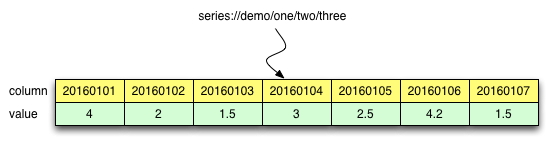
\includegraphics[scale=0.7]{Graphics/SeriesExplain}
\caption{Rapture Series Structure}
\label{fig:RaptureSeriesStructure}
\end{figure}

Figure~\vref{fig:RaptureSeriesStructure} shows the association between a series uri in \Rapture and the data
it "points" to.

\subsection{Blob Data}

Blob (Binary Large OBject) data is used in \Rapture to store data that has some structure or value to an
external application but has no real "meaning" internally to \Rapture. The uri reference to a blob in \Rapture
points to a sequence of bytes -- \Rapture understands (and maintains) the mime-type of the data and its length
and other attributes such as the last writer and write time but it is really just an arbitary store of information.

\Rapture applications tend to use Blob repositories to store spreadsheets, cvs files, images, application code and the like.

\begin{figure}[htb]
\centering
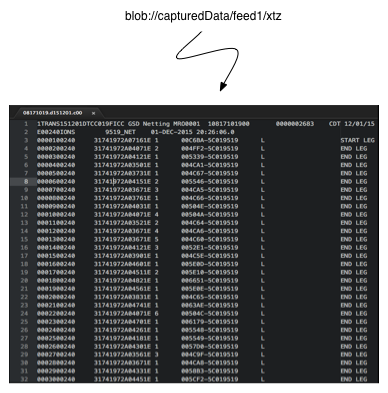
\includegraphics[scale=0.75]{Graphics/RaptureBlobExplain}
\caption{Rapture Blob Structure}
\label{fig:RaptureBlobStructure}
\end{figure}

Figure~\vref{fig:RaptureBlobStructure} shows an example blob uri pointing to a csv file
used in an import/processing application.

\subsection{Structured Data}

Structured data is an alias for "relational data". Structured repositories (equivalent to databases and tables in
a relational database) are used in two completely different ways.

\subsubsection{Internal Structured Data}

A structured data repository can be used internally within an application to store information that is relational in
layout -- the internal reference implies that applications only modify and access this information through the \Rapture API. With
this restriction \Rapture can manage server side caching of the information and propogate changes in a distributed manner to
other servers in a \Rapture environment.

\subsubsection{External Structured Data}

An external structured data repository is simply a well described connection to an external database (and table set). The idea
is that applications and process that are using other \Rapture facilities (the other data types described here, workflows etc.) can
treat this type of external data in the same manner and have a single mechanism for accessing and joining these disparate data sets. In addition
the entitlements system of \Rapture can be used to control access to such a resource.

\section{Workflows}

With data under control with a consistent access mechanism and naming conventions there is often a need in an enterprise application to
manipulate and transform this data in consistent ways. Programs that manipulate data (or do other tasks) can often be broken down into a set of steps
and a workflow in \Rapture is a vehicle for managing the execution of those steps in a controlled and distributed manner.

A sample workflow in \Rapture is shown in Figure~\vref{fig:WorkflowExample}.

\begin{figure}[H]
\centering
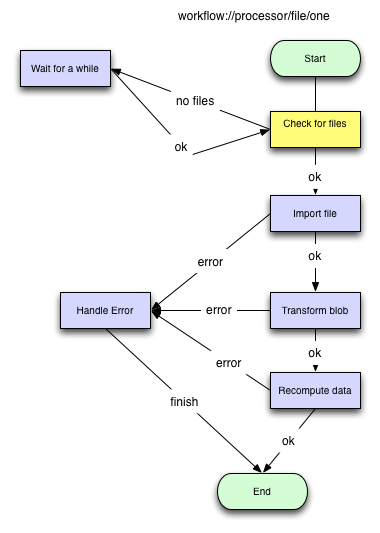
\includegraphics[scale=0.75]{Graphics/RaptureWorkflowExplain}
\caption{Rapture Workflow}
\label{fig:WorkflowExample}
\end{figure}

This workflow, with the unique reference "workflow://processor/file/one" begins at the start step. The first
task (or step) that is executed is "Check for Files". The implementation of a step in a \Rapture workflow can be either
a piece of Java code that is embedded in the \Rapture server (as shown as a workflow extension in Figure~\vref{fig:RaptureExtensionPoints})
or can be a \Reflex script hosted on \Rapture itself. After doing its work the step execution code returns a status code - a piece of text
that is used to point to the next step that will be executed. In this case returning "ok" will move it to the "import file" step and returning
"no files" can point it to the "wait for a while" step. These steps execute in a similar way and the workflow execution continues until we
reach the "End" point.

In a real workflow the "Wait for a while" step would ultimately error out after an extended time.

Workflow steps are associated with server groups and any server in a group can be used to process that step. In this example the yellow first step
needs to run on a special server that has access to a specific file location - once the file(s) are located they are imported into a \Rapture blob repository
and the other steps can run on any server in the environment. This technique and approach allows \Rapture workflows to be distributed across a compute fabric while
still maintaining some constraints on execution.

Workflows can be started (run) using the \Rapture API (see the Decision API later on in this document) or attached to events or schedules.

\section{Scripts}

Scripts in \Rapture refer to programs written in the \Reflex scripting language. That language is described later on in this document.

Scripts have unique references (uris) in \Rapture and can be used in many different ways. Some of the typical use cases are enumerated below:

\begin{itemize}
	\item{Workflow steps can use scripts as part of their execution.}
	\item{Scripts can be run one-off as mini-programs through the \Rapture API.}
	\item{Scripts can be run upon an event firing.}
	\item{Scripts can be executed as part of an AJAX call to a service -- usually returning JSON data controlled by parameters passed in the service call.}
\end{itemize}

\section{Pipelines and Messages}
\Rapture can be a multi-server environment. Coordination is needed between individual servers and this is accomplished through messaging. These messages are
used to coordinate workflow activity or the initiation of any asynchronous style activity. \Rapture abstracts the concept of messaging and message queues from their
implementation. The \Rapture kernel requires at least one of these "pipelines" to be setup for a system to run. In a single server environment
this could be an in memory (in process) implementation - in a multi-server environment the open source RabbitMQ implementation is recommended.

Figure~\vref{fig:PipelineExample} shows the different types of pipeline that could exist in a \Rapture environment.

\begin{figure}[H]
\centering
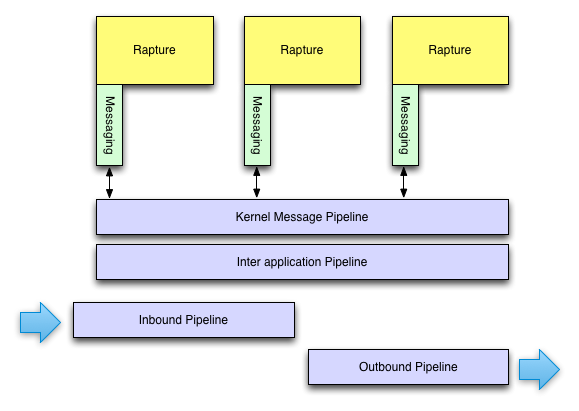
\includegraphics[scale=0.75]{Graphics/PipelineExplain}
\caption{Rapture Pipeline}
\label{fig:PipelineExample}
\end{figure}

The same pipeline system can be used by applications as well. Applications create queues on exchanges and can be both a publisher and a consumer of custom messages
sent on those queues. Some queues could have no endpoint within \Rapture -- they could imply connectivity to external applications and systems. Conversely such queues could
represent inbound queues from external systems. This abstraction separates the application code (the publisher and consumer) from the actual implementation of the transport.


\section{Jobs and Schedules}

In a \Rapture environment running a batch process in a production context it is often required to scheduled repeating tasks in a consistent manner.

\Rapture has the concept of a schedule manager where you can define jobs that can execute according to the evaluation of a cron style specification. These jobs
can be used to run scripts or workflows and there are many operational style API calls that can be used to monitor their progress.


\chapter{Application Locations}
Applications interacting with \Rapture will typicall fall within one of the
following categories.

\begin{itemize}
  \item{Client applications interacting with a remote \Rapture environment.}
  \item{Client \Reflex scripts using the ReflexRunner application. These behave like client applications as far as \Rapture is concerned.}
  \item{Server applications embedding the \Rapture kernel.}
  \item{Scripts running on a server that is itself running the \Rapture kernel.}
  \item{Extensions to \Reflex or repository or message drivers.}
  \item{Scripts run in the context of an ajax call from a web browser.}
\end{itemize}

\begin{figure}[H]
\centering
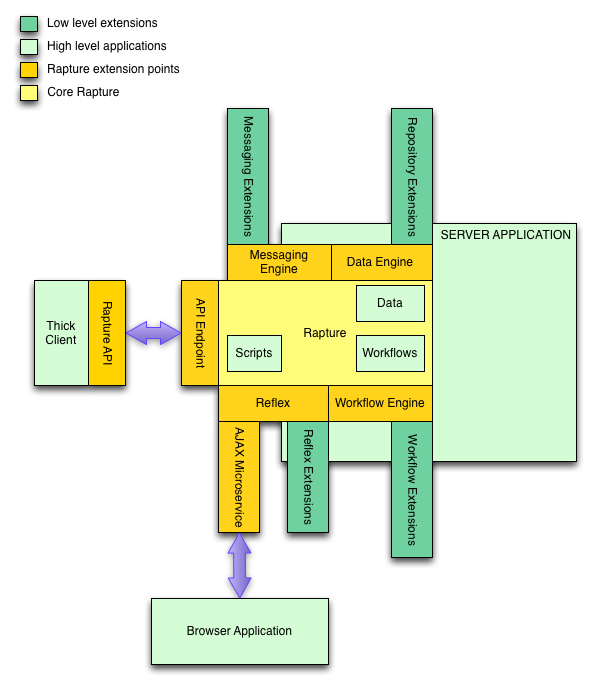
\includegraphics[scale=0.75]{Graphics/RaptureExtensionPoints}
\caption{Rapture Extension Points}
\label{fig:RaptureExtensionPoints}
\end{figure}

The diagram of Figure~\vref{fig:RaptureExtensionPoints} shows the places in which these extensions can take
place. Typically a \Rapture environment or application suite is a combination of some of these -- and Incapture Technologies
can provide some enterprise extensions (particularly in the low level extensions space) that can assist in rounding out an
application.

\section{Context and Entitlements}
Every interaction with a \Rapture API call is made in the context of a logged in
user. That user, and its entitlement group membership and the parameters passed
to the call are used to determine whether the call can proceed or not. If an
API call is used to run a script on \Rapture or to start a workflow \emph{that} script
or workflow is run in the context of the calling user as well.

In some API use categories the interface used to interact with the \Rapture API
is already bound to a user - typically this is for processes that are running
server side. Client side use cases usually have to \emph{login} to \Rapture first,
providing credentials that get translated by the \Rapture API into a \verb+CallingContext+
value (a token) which can then be used in subsequent calls to identify the user
making the call. In some client side languages there are helper constructs that
can be used to automatically pass in the logged in context to the API calls,
leaving the programmer free to not worry about this aspect.

Wrapper applications such as ReflexRunner log in on the caller's behalf and then
pass that logged in API context to the underlying container that runs the script.

\section{Custom client applications}

Client applications that talk to \Rapture can be written in any of these supported languages as
long as the application can reach (using TCP/IP) a \Rapture API Server.

\begin{itemize}
  \item{Java (or anything that runs on the Java VM and can access Java classes.)}
  \item{.NET}
  \item{Python}
  \item{Javascript (typically node.js, see a later section on architectures for browser applications.)}
  \item{Ruby}
  \item{Go(lang)}
\end{itemize}

The transport between client and server uses a JSON-RPC style of communication which
means that other language support can easily be added. The build process for
\Rapture can autogenerate client side stubs once an initial template has been
created - the authors created the .NET implementation in a few hours.

Typically the use of \Rapture in these applications follows this pattern:

\begin{enumerate}
  \item{Obtain the ip address or name of the \Rapture environment API endpoint.}
  \item{Obtain the user name and password for the use of the API.}
  \item{Call a login function to obtain a calling context.}
  \item{Pass that login context into a wrapper (for future API use) or simply pass the context into future API calls.}
\end{enumerate}

For example in Java here is a simple code extract for the login and API use process:

\begin{lstlisting}[caption={Java simple example}, language=Java]
  String host = "test.incapture.net";
  String username = "test";
  String password = "secret";
  SimpleCredentialsProvider creds = new SimpleCredentialsProvider(username, password);
  HttpLoginApi loginApi = new HttpLoginApi(host, creds);
  loginApi.login();

  ScriptClient client = new ScriptClient(loginApi);
  String content = client.getDoc().getContent("//testRepo/doc/one");
  System.out.println(content);
\end{lstlisting}

This example logs into a \Rapture environment and passes that logged in context to a \verb+ScriptClient+
instance. It is this script client that can then be easily used to interact with \Rapture. The
\verb+getContent+ call in the document API will be described in detail later.

In Python, the equivalent interaction is reproduced below:

\begin{lstlisting}[caption={Python simple example}, language=Python]
  import raptureAPI
  url = 'test.incapture.net'
  username = 'test'
  password = 'secret'
  rapture = raptureAPI.raptureAPI(url, username, password)
  content = rapture.doDoc_GetContent('//testRepo/doc/one')
  print content
\end{lstlisting}

Here we see a similar login approach and then the invocation of the same \Rapture
API call. With the same target \Rapture environment these two code snippets will
produce exactly the same output.

\section{Client Reflex scripts}

\Reflex scripts running on the client (or the server) are always running in a
container that has already been connected to an environment -- the wrapper is
the piece of code that has logged into \Rapture already.

In \Reflex then the code is even simpler. In fact \Reflex has some additional
syntax sugar for loading documents from \Rapture.

\begin{lstlisting}[caption={Reflex simple example}, language=reflex]
  contentAsMap <-- "//testRepo/doc/one";
  println(contentAsMap);

  // or

  content = #doc.getContent("//testRepo/doc/one");
  contentAsMap = fromjson(content);
  println(contentAsMap);
\end{lstlisting}

In the second access example we convert the raw JSON formatted document from
\Rapture into a \Reflex map structure so as to make the two approaches produce
the same output.

\section{Server side kernel applications}

If a Java (or Java VM) application embeds the \Rapture kernel code within it the
means for calling the \Rapture API can have a number of forms. Code running within
\Rapture has to be much more careful about calling contexts and who is actually
making the call, and there is no need to worry about host urls because the code
is running directly on \Rapture.

One approach to running the same example code is reproduced below:

\begin{lstlisting}[caption={Kernel simple example}, language=Java]
   CallingContext userContext = Kernel.getLogin().login(
          "test", "secret", null);
   String content = Kernel.getDoc().getContent(
          userContext, "//testRepo/doc/one");
   System.out.println(content);
\end{lstlisting}

Note that to run the above code your server application will have had to initialize
and configure itself first, something which is outside the scope of this document
but will trivially be a matter of defining configuration files for connection to
underlying data stores and then calling:

\begin{lstlisting}[caption={Kernel initialization}, language=Java]
   Kernel.initBootstrap();
\end{lstlisting}

\part{API}
\chapter{API Introduction}
The \Rapture API is divided into a number of sections. We've seen in an earlier
section how you may need to use the \emph{login} api to establish a connection
to \Rapture. The other sections of the API will form the rest of this document.
For each section the general positioning of the section with respect to \Rapture
will be described and then the detailed API calls will follow.

\chapter{Doc API}
\index{Doc API}
The Structured API is used to manage interactions with external relational databases. The set
of API calls matches most of those provided through a standard JDBC style interface except that where
possible the calls rely on URIs to either define consistent access points to data or to define consistent
techniques for updating that data.

There are two ways to use this API. The first is to manage interaction with a private (to \Rapture) database
for the purpose of an internal application. Many of the more management API calls are provided for this purpose. The
second is for interaction with an existing external database that is maintained external to the \Rapture system. The data style
calls are more relevant for this access -- the management api calls would likely fail to execute due to authorization restrictions.

\subsection{ValidateDocRepo}
\index{ValidateDocRepo}
\label{Api:ValidateDocRepo}
\begin{Verbatim}
   boolean validateDocRepo (
           String    docRepoUri
   )
\end{Verbatim}
\begin{Verbatim}[formatcom=\color{Maroon}]
  Entitlement: /repo/write
\end{Verbatim}
%\begin{lstlisting}[language=reflex]
%ret = #doc.validateDocRepo(docRepoUri);
%\end{lstlisting}
\input{doc/validateDocRepo}


\rule{12cm}{2pt}
\subsection{CreateDocRepo}
\index{CreateDocRepo}
\label{Api:CreateDocRepo}
\begin{Verbatim}
   void createDocRepo (
           String    docRepoUri
           String    config
   )
\end{Verbatim}
\begin{Verbatim}[formatcom=\color{Maroon}]
  Entitlement: /repo/write
\end{Verbatim}
%\begin{lstlisting}[language=reflex]
%ret = #doc.createDocRepo(docRepoUri,config);
%\end{lstlisting}
The \verb+createDocRepo+ is used to create a new document repository in \Rapture. The parameters to the call
look straightforward -- simply the name of the new repository and a configuration string. The configuration string is
in fact a complex instruction written in a repository domain specific language (DSL) that is used to define the
capabilities and underlying implementation of the repository.

The typical configuration string for a versioned repository backed by MongoDB is reproduced below:

\begin{Verbatim}
NREP {} USING MONGODB { prefix = 'test' }
\end{Verbatim}

The general form of the configuration is:

\begin{Verbatim}
[type of document repo] { [ document repo config] }
     USING [underlying implementation] { [ config ]}
     [ ON [ instance] ]
\end{Verbatim}

The first part, the type of the document repo, can be either \verb+NREP+ or \verb+REP+. The former
indicates that a versioned repository should be created, the latter that an unversioned repository
should be created.

The document repo config part of the configuration string is currently blank for all document repo types.

The second part of the configuration string defines the underlying implementation and its configuration. In
most cases the configuration associated with the implementation has a \verb+prefix+ parameter that is used to
define a table or a collection or a prefix for such entities in the underlying storage. The underlying implementation
defines what lower level software is used to host the data managed by \Rapture. The following table shows the current
implementations:

\begin{table}[H]
\small
\begin{center}
\begin{tabular}{r l p{8cm}}
  Keyword & Underlying & Configuration \\
  \hline
  MONGODB & MongoDb & The prefix parameter defines the name of the collections used by this repository. To avoid
  conflict this is usually a function of the name of the \Rapture repository. \\
  CASSANDRA & Cassandra & The prefix parameter defines the name of the collections used by this repository. To avoid
  conflict this is usually a function of the name of the \Rapture repository. \\
  POSTGRES & PostgresSql &  The prefix parameter defines the name of the tables used by this repository. To avoid
  conflict this is usually a function of the name of the \Rapture repository. \\
\end{tabular}
\end{center}
\end{table}

Incapture has additional implementations of document repositories for Oracle, JDBC, Redis, ehCache and memcached.

There are some additional directives that can be used in a repository configuration definition.

If the keyword \verb+READONLY+ is used at the start of the configuration (e.g. \verb+READONLY NREP ...+) the repository will
be readonly -- it is assumed that either a different repository configuration is used to write data (and they
share the same \verb+preifx+ but different entitlements) or the underlying data in a repository is a backup of
a repository created with a different system. In any case the \verb+READONLY+ keyword makes all writing API calls to
this repository fail with an exception being thrown.

The \verb+ON+ directive defines which configuration will be used to connect to the underlying store. If
not present the \verb+DEFAULT+ configuration will be used. These keywords are used by the underlying
implementation to load a system specific configuration file, environment variables or property set.

For example the default configuration for MongoDb (\verb+ON DEFAULT+) instructs the MongoDB implementation
to look in three places for a connection string to a MongoDB server -

\begin{itemize}
\item{The environment variable RAPTUREMONGODB-DEFAULT.}
\item{The java property RAPTUREMONGODB-DEFAULT.}
\item{The line beginning default= in the file RaptureMONGODB.cfg on the classpath of the application.}
\end{itemize}

In most cases the implementation will read the value from the file associated with the application server.

Using this technique multiple underlying servers can be used and repositories attached to them using the
\verb+ON+ keyword.



\rule{12cm}{2pt}
\subsection{DocRepoExists}
\index{DocRepoExists}
\label{Api:DocRepoExists}
\begin{Verbatim}
   boolean docRepoExists (
           String    docRepoUri
   )
\end{Verbatim}
\begin{Verbatim}[formatcom=\color{Maroon}]
  Entitlement: /repo/list
\end{Verbatim}
%\begin{lstlisting}[language=reflex]
%ret = #doc.docRepoExists(docRepoUri);
%\end{lstlisting}
\input{doc/docRepoExists}


\rule{12cm}{2pt}
\subsection{DocExists}
\index{DocExists}
\label{Api:DocExists}
\begin{Verbatim}
   boolean docExists (
           String    docUri
   )
\end{Verbatim}
\begin{Verbatim}[formatcom=\color{Maroon}]
  Entitlement: /repo/list
\end{Verbatim}
%\begin{lstlisting}[language=reflex]
%ret = #doc.docExists(docUri);
%\end{lstlisting}
\input{doc/docExists}


\rule{12cm}{2pt}
\subsection{GetDocRepoConfig}
\index{GetDocRepoConfig}
\label{Api:GetDocRepoConfig}
\begin{Verbatim}
   DocumentRepoConfig getDocRepoConfig (
           String    docRepoUri
   )
\end{Verbatim}
\begin{Verbatim}[formatcom=\color{Maroon}]
  Entitlement: /repo/read
\end{Verbatim}
%\begin{lstlisting}[language=reflex]
%ret = #doc.getDocRepoConfig(docRepoUri);
%\end{lstlisting}
The \verb+getDocRepoConfig+ api call returns the underlying structure of a document repository. The return
value is a complex type that has the following fields:

\begin{table}[h]
  \small
\begin{center}
\begin{tabular}{r l p{7cm}}
  Field & Type & Description \\
  \hline
  description & String & The description of this repository. \\
  config & String & The configuration passed to the createDocRepo call. \\
  authority & String & No longer used. \\
  idGenUri & String & If the repository uses an autogenerated id mechanism this is the implementation to use. (See IDs) \\
  strictCheck & Boolean & If set the repository will validate documents as a JSON format before saving. \\
  indexes & Set<IndexScriptPair> & defined if there are any indices associated with this repository (see Indexes). \\
  documentRepo & RaptureDocConfig & a repeat of the information stored in the authority and config sections. \\
\end{tabular}
\end{center}
\end{table}



\rule{12cm}{2pt}
\subsection{GetDocRepoStatus}
\index{GetDocRepoStatus}
\label{Api:GetDocRepoStatus}
\begin{Verbatim}
   Map<String,String> getDocRepoStatus (
           String    docRepoUri
   )
\end{Verbatim}
\begin{Verbatim}[formatcom=\color{Maroon}]
  Entitlement: /repo/read
\end{Verbatim}
%\begin{lstlisting}[language=reflex]
%ret = #doc.getDocRepoStatus(docRepoUri);
%\end{lstlisting}
\input{doc/getDocRepoStatus}


\rule{12cm}{2pt}
\subsection{GetDocRepoConfigs}
\index{GetDocRepoConfigs}
\label{Api:GetDocRepoConfigs}
\begin{Verbatim}
   List<DocumentRepoConfig> getDocRepoConfigs (
   )
\end{Verbatim}
\begin{Verbatim}[formatcom=\color{Maroon}]
  Entitlement: /repo/read
\end{Verbatim}
%\begin{lstlisting}[language=reflex]
%ret = #doc.getDocRepoConfigs();
%\end{lstlisting}
\input{doc/getDocRepoConfigs}


\rule{12cm}{2pt}
\subsection{DeleteDocRepo}
\index{DeleteDocRepo}
\label{Api:DeleteDocRepo}
\begin{Verbatim}
   void deleteDocRepo (
           String    docRepoUri
   )
\end{Verbatim}
\begin{Verbatim}[formatcom=\color{Maroon}]
  Entitlement: /repo/write
\end{Verbatim}
%\begin{lstlisting}[language=reflex]
%ret = #doc.deleteDocRepo(docRepoUri);
%\end{lstlisting}
\input{doc/deleteDocRepo}


\rule{12cm}{2pt}
\subsection{ArchiveRepoDocs}
\index{ArchiveRepoDocs}
\label{Api:ArchiveRepoDocs}
\begin{Verbatim}
   void archiveRepoDocs (
           String    docRepoUri
           int    versionLimit
           long    timeLimit
           boolean    ensureVersionLimit
   )
\end{Verbatim}
\begin{Verbatim}[formatcom=\color{Maroon}]
  Entitlement: /repo/write
\end{Verbatim}
%\begin{lstlisting}[language=reflex]
%ret = #doc.archiveRepoDocs(docRepoUri,versionLimit,timeLimit,ensureVersionLimit);
%\end{lstlisting}
The \verb+archiveRepoDocs+ call removes older versions of documents from a
repository that match certain criteria.

\begin{table}[H]
  \small
\begin{center}
\begin{tabular}{r p{8cm}}
  Parameter & Purpose \\
  \hline
  docRepoUri & If this document uri contains just the name of a repository then all
  documents in the repository will be checked. Otherwise just those matching this prefix will be
  scanned. \\
  versionLimit & If the ensureVersionLimit parameter is true this parameter will determine
  the minimum number of versions to keep fora document. \\
  timeLimit & This parameter determines the modification time of the oldest version to keep during this
  archive process. \\
  ensureVersionLimit & If this parameter is true the versionLimit parameter is used \\
\end{tabular}
\end{center}
\end{table}



\rule{12cm}{2pt}
\subsection{GetDocAndMeta}
\index{GetDocAndMeta}
\label{Api:GetDocAndMeta}
\begin{Verbatim}
   DocumentWithMeta getDocAndMeta (
           String    docUri
   )
\end{Verbatim}
\begin{Verbatim}[formatcom=\color{Maroon}]
  Entitlement: /data/read/$f(docUri)
\end{Verbatim}
%\begin{lstlisting}[language=reflex]
%ret = #doc.getDocAndMeta(docUri);
%\end{lstlisting}
The \verb+getDocAndMeta+ API call is used to retrieve both the content of
a document and the meta data associated with that document. If the uri does
not have a version qualifier the information returned will refer to the latest
version of the document. The return value is complex is structure -- please
refer to the table at the end of this section to understand the fields within that
structure.

The \verb+DocumentWithMeta+ return value is a complex structure that contains
the following fields:

\begin{table}[H]
  \small
\begin{center}
\begin{tabular}{rl p{7cm}}
  Field & Type & Description \\
  \hline
  displayName & String & the url of this document \\
  metaData & DocumentMetaData & the metadata associated with this document \\
  content & String & the content of this document \\
\end{tabular}
\end{center}
\end{table}



\rule{12cm}{2pt}
\subsection{GetDocMeta}
\index{GetDocMeta}
\label{Api:GetDocMeta}
\begin{Verbatim}
   DocumentMetadata getDocMeta (
           String    docUri
   )
\end{Verbatim}
\begin{Verbatim}[formatcom=\color{Maroon}]
  Entitlement: /data/list/$f(docUri)
\end{Verbatim}
%\begin{lstlisting}[language=reflex]
%ret = #doc.getDocMeta(docUri);
%\end{lstlisting}
The \verb+getDocMeta+ API call is used to retrieve the meta data associated
with a given document in a repository. If the uri does not have a version
qualifier the information returned will refer to the latest version of the
document. The return value is complex is structure -- please refer to the
table at the end of this section to understand the fields within that
structure.

The \verb+DocumentMetaData+ return value is a complex structure that contains
the following fields:

\begin{table}[H]
  \small
\begin{center}
\begin{tabular}{rl p{8cm}}
  Field & Type & Description \\
  \hline
  version & integer & the version number of this document \\
  createdTimestamp & long & when this document was first created \\
  modifiedTimestamp & long & when this document was last modified \\
  user & string & the user that made this modification \\
  comment & string & any comment that was provided when the document was written \\
  deleted & boolean & whether this document is deleted \\
\end{tabular}
\end{center}
\end{table}



\rule{12cm}{2pt}
\subsection{RevertDoc}
\index{RevertDoc}
\label{Api:RevertDoc}
\begin{Verbatim}
   DocumentWithMeta revertDoc (
           String    docUri
   )
\end{Verbatim}
\begin{Verbatim}[formatcom=\color{Maroon}]
  Entitlement: /data/write/$f(docUri)
\end{Verbatim}
%\begin{lstlisting}[language=reflex]
%ret = #doc.revertDoc(docUri);
%\end{lstlisting}
\input{doc/revertDoc}


\rule{12cm}{2pt}
\subsection{GetDoc}
\index{GetDoc}
\label{Api:GetDoc}
\begin{Verbatim}
   String getDoc (
           String    docUri
   )
\end{Verbatim}
\begin{Verbatim}[formatcom=\color{Maroon}]
  Entitlement: /data/read/$f(docUri)
\end{Verbatim}
%\begin{lstlisting}[language=reflex]
%ret = #doc.getDoc(docUri);
%\end{lstlisting}
\input{doc/getDoc}


\rule{12cm}{2pt}
\subsection{PutDoc}
\index{PutDoc}
\label{Api:PutDoc}
\begin{Verbatim}
   String putDoc (
           String    docUri
           String    content
   )
\end{Verbatim}
\begin{Verbatim}[formatcom=\color{Maroon}]
  Entitlement: /data/write/$f(docUri)
\end{Verbatim}
%\begin{lstlisting}[language=reflex]
%ret = #doc.putDoc(docUri,content);
%\end{lstlisting}
\input{doc/putDoc}


\rule{12cm}{2pt}
\subsection{PutDocWithVersion}
\index{PutDocWithVersion}
\label{Api:PutDocWithVersion}
\begin{Verbatim}
   boolean putDocWithVersion (
           String    docUri
           String    content
           int    currentVersion
   )
\end{Verbatim}
\begin{Verbatim}[formatcom=\color{Maroon}]
  Entitlement: /data/write/$f(docUri)
\end{Verbatim}
%\begin{lstlisting}[language=reflex]
%ret = #doc.putDocWithVersion(docUri,content,currentVersion);
%\end{lstlisting}
\input{doc/putDocWithVersion}


\rule{12cm}{2pt}
\subsection{PutDocWithEventContext}
\index{PutDocWithEventContext}
\label{Api:PutDocWithEventContext}
\begin{Verbatim}
   DocWriteHandle putDocWithEventContext (
           String    docUri
           String    content
           Map<String,String>    eventContext
   )
\end{Verbatim}
\begin{Verbatim}[formatcom=\color{Maroon}]
  Entitlement: /data/write/$f(docUri)
\end{Verbatim}
%\begin{lstlisting}[language=reflex]
%ret = #doc.putDocWithEventContext(docUri,content,eventContext);
%\end{lstlisting}
\input{doc/putDocWithEventContext}


\rule{12cm}{2pt}
\subsection{DeleteDoc}
\index{DeleteDoc}
\label{Api:DeleteDoc}
\begin{Verbatim}
   boolean deleteDoc (
           String    docUri
   )
\end{Verbatim}
\begin{Verbatim}[formatcom=\color{Maroon}]
  Entitlement: /data/write/$f(docUri)
\end{Verbatim}
%\begin{lstlisting}[language=reflex]
%ret = #doc.deleteDoc(docUri);
%\end{lstlisting}
\input{doc/deleteDoc}


\rule{12cm}{2pt}
\subsection{RenameDoc}
\index{RenameDoc}
\label{Api:RenameDoc}
\begin{Verbatim}
   String renameDoc (
           String    fromDocUri
           String    toDocUri
   )
\end{Verbatim}
\begin{Verbatim}[formatcom=\color{Maroon}]
  Entitlement: /data/write/$f(fromDocUri)
\end{Verbatim}
%\begin{lstlisting}[language=reflex]
%ret = #doc.renameDoc(fromDocUri,toDocUri);
%\end{lstlisting}
\input{doc/renameDoc}


\rule{12cm}{2pt}
\subsection{GetDocs}
\index{GetDocs}
\label{Api:GetDocs}
\begin{Verbatim}
   Map<String,String> getDocs (
           List<String>    docUris
   )
\end{Verbatim}
\begin{Verbatim}[formatcom=\color{Maroon}]
  Entitlement: /data/batch
\end{Verbatim}
%\begin{lstlisting}[language=reflex]
%ret = #doc.getDocs(docUris);
%\end{lstlisting}
\input{doc/getDocs}


\rule{12cm}{2pt}
\subsection{GetDocAndMetas}
\index{GetDocAndMetas}
\label{Api:GetDocAndMetas}
\begin{Verbatim}
   List<DocumentWithMeta> getDocAndMetas (
           List<String>    docUris
   )
\end{Verbatim}
\begin{Verbatim}[formatcom=\color{Maroon}]
  Entitlement: /data/batch
\end{Verbatim}
%\begin{lstlisting}[language=reflex]
%ret = #doc.getDocAndMetas(docUris);
%\end{lstlisting}
\input{doc/getDocAndMetas}


\rule{12cm}{2pt}
\subsection{DocsExist}
\index{DocsExist}
\label{Api:DocsExist}
\begin{Verbatim}
   List<boolean> docsExist (
           List<String>    docUris
   )
\end{Verbatim}
\begin{Verbatim}[formatcom=\color{Maroon}]
  Entitlement: /data/batch
\end{Verbatim}
%\begin{lstlisting}[language=reflex]
%ret = #doc.docsExist(docUris);
%\end{lstlisting}
\input{doc/docsExist}


\rule{12cm}{2pt}
\subsection{PutDocs}
\index{PutDocs}
\label{Api:PutDocs}
\begin{Verbatim}
   List<Object> putDocs (
           List<String>    docUris
           List<String>    contents
   )
\end{Verbatim}
\begin{Verbatim}[formatcom=\color{Maroon}]
  Entitlement: /data/batch
\end{Verbatim}
%\begin{lstlisting}[language=reflex]
%ret = #doc.putDocs(docUris,contents);
%\end{lstlisting}
\input{doc/putDocs}


\rule{12cm}{2pt}
\subsection{RenameDocs}
\index{RenameDocs}
\label{Api:RenameDocs}
\begin{Verbatim}
   List<String> renameDocs (
           String    authority
           String    comment
           List<String>    fromDocUris
           List<String>    toDocUris
   )
\end{Verbatim}
\begin{Verbatim}[formatcom=\color{Maroon}]
  Entitlement: /data/batch
\end{Verbatim}
%\begin{lstlisting}[language=reflex]
%ret = #doc.renameDocs(authority,comment,fromDocUris,toDocUris);
%\end{lstlisting}
\input{doc/renameDocs}


\rule{12cm}{2pt}
\subsection{DeleteDocsByUriPrefix}
\index{DeleteDocsByUriPrefix}
\label{Api:DeleteDocsByUriPrefix}
\begin{Verbatim}
   List<String> deleteDocsByUriPrefix (
           String    docUri
   )
\end{Verbatim}
\begin{Verbatim}[formatcom=\color{Maroon}]
  Entitlement: /data/write/$f(docUri)
\end{Verbatim}
%\begin{lstlisting}[language=reflex]
%ret = #doc.deleteDocsByUriPrefix(docUri);
%\end{lstlisting}
\input{doc/deleteDocsByUriPrefix}


\rule{12cm}{2pt}
\subsection{ListDocsByUriPrefix}
\index{ListDocsByUriPrefix}
\label{Api:ListDocsByUriPrefix}
\begin{Verbatim}
   Map<String,RaptureFolderInfo> listDocsByUriPrefix (
           String    docUri
           int    depth
   )
\end{Verbatim}
\begin{Verbatim}[formatcom=\color{Maroon}]
  Entitlement: /data/read/$f(docUri)
\end{Verbatim}
%\begin{lstlisting}[language=reflex]
%ret = #doc.listDocsByUriPrefix(docUri,depth);
%\end{lstlisting}
The \verb+listDocsByUriPrefix+ call is normally used by user interfaces that wish
to present a browser type interface on a document repository. The call returns all documents
and "sub folders" (to a given depth) below a given point in the hierarchy implied
by the naming conventions used in uris. Typically an interface will use \verb+/+ as
the initial prefix and then append onto that prefix the names of either documents
or folders for further \verb+listDocs+ type calls or \verb+getDoc+ if the location
maps to a real document.

The \verb+RaptureFolderInfo+ structure returned by this call is described below:

\begin{table}[H]
  \small
\begin{center}
\begin{tabular}{r l p{8cm}}
  Field & Type & Description \\
  \hline
  name & String & The name of this element. \\
  folder & Boolean & Whether the name refers to a document or a sub-folder \\
\end{tabular}
\end{center}
\end{table}



\rule{12cm}{2pt}
\subsection{SetDocAttribute}
\index{SetDocAttribute}
\label{Api:SetDocAttribute}
\begin{Verbatim}
   boolean setDocAttribute (
           String    attributeUri
           String    value
   )
\end{Verbatim}
\begin{Verbatim}[formatcom=\color{Maroon}]
  Entitlement: /data/write/$f(attributeUri)
\end{Verbatim}
%\begin{lstlisting}[language=reflex]
%ret = #doc.setDocAttribute(attributeUri,value);
%\end{lstlisting}
\input{doc/setDocAttribute}


\rule{12cm}{2pt}
\subsection{SetDocAttributes}
\index{SetDocAttributes}
\label{Api:SetDocAttributes}
\begin{Verbatim}
   Map<String,boolean> setDocAttributes (
           String    attributeUri
           List<String>    keys
           List<String>    values
   )
\end{Verbatim}
\begin{Verbatim}[formatcom=\color{Maroon}]
  Entitlement: /data/write/$f(attributeUri)
\end{Verbatim}
%\begin{lstlisting}[language=reflex]
%ret = #doc.setDocAttributes(attributeUri,keys,values);
%\end{lstlisting}
\input{doc/setDocAttributes}


\rule{12cm}{2pt}
\subsection{GetDocAttribute}
\index{GetDocAttribute}
\label{Api:GetDocAttribute}
\begin{Verbatim}
   XferDocumentAttribute getDocAttribute (
           String    attributeUri
   )
\end{Verbatim}
\begin{Verbatim}[formatcom=\color{Maroon}]
  Entitlement: /data/read/$f(attributeUri)
\end{Verbatim}
%\begin{lstlisting}[language=reflex]
%ret = #doc.getDocAttribute(attributeUri);
%\end{lstlisting}
\input{doc/getDocAttribute}


\rule{12cm}{2pt}
\subsection{GetDocAttributes}
\index{GetDocAttributes}
\label{Api:GetDocAttributes}
\begin{Verbatim}
   List<XferDocumentAttribute> getDocAttributes (
           String    attributeUri
   )
\end{Verbatim}
\begin{Verbatim}[formatcom=\color{Maroon}]
  Entitlement: /data/read/$f(attributeUri)
\end{Verbatim}
%\begin{lstlisting}[language=reflex]
%ret = #doc.getDocAttributes(attributeUri);
%\end{lstlisting}
\input{doc/getDocAttributes}


\rule{12cm}{2pt}
\subsection{DeleteDocAttribute}
\index{DeleteDocAttribute}
\label{Api:DeleteDocAttribute}
\begin{Verbatim}
   boolean deleteDocAttribute (
           String    attributeUri
   )
\end{Verbatim}
\begin{Verbatim}[formatcom=\color{Maroon}]
  Entitlement: /data/write/$f(attributeUri)
\end{Verbatim}
%\begin{lstlisting}[language=reflex]
%ret = #doc.deleteDocAttribute(attributeUri);
%\end{lstlisting}
\input{doc/deleteDocAttribute}


\rule{12cm}{2pt}
\subsection{GetDocRepoIdGenUri}
\index{GetDocRepoIdGenUri}
\label{Api:GetDocRepoIdGenUri}
\begin{Verbatim}
   String getDocRepoIdGenUri (
           String    docRepoUri
   )
\end{Verbatim}
\begin{Verbatim}[formatcom=\color{Maroon}]
  Entitlement: /admin/idgen
\end{Verbatim}
%\begin{lstlisting}[language=reflex]
%ret = #doc.getDocRepoIdGenUri(docRepoUri);
%\end{lstlisting}
\input{doc/getDocRepoIdGenUri}


\rule{12cm}{2pt}
\subsection{SetDocRepoIdGenConfig}
\index{SetDocRepoIdGenConfig}
\label{Api:SetDocRepoIdGenConfig}
\begin{Verbatim}
   DocumentRepoConfig setDocRepoIdGenConfig (
           String    docRepoUri
           String    idGenConfig
   )
\end{Verbatim}
\begin{Verbatim}[formatcom=\color{Maroon}]
  Entitlement: /admin/idgen
\end{Verbatim}
%\begin{lstlisting}[language=reflex]
%ret = #doc.setDocRepoIdGenConfig(docRepoUri,idGenConfig);
%\end{lstlisting}
\input{doc/setDocRepoIdGenConfig}


\rule{12cm}{2pt}
\subsection{GetDocRepoIdGenConfig}
\index{GetDocRepoIdGenConfig}
\label{Api:GetDocRepoIdGenConfig}
\begin{Verbatim}
   RaptureIdGenConfig getDocRepoIdGenConfig (
           String    docRepoUri
   )
\end{Verbatim}
\begin{Verbatim}[formatcom=\color{Maroon}]
  Entitlement: /admin/idgen
\end{Verbatim}
%\begin{lstlisting}[language=reflex]
%ret = #doc.getDocRepoIdGenConfig(docRepoUri);
%\end{lstlisting}
\input{doc/getDocRepoIdGenConfig}


\rule{12cm}{2pt}

\chapter{Blob API}
\index{Blob API}
The Structured API is used to manage interactions with external relational databases. The set
of API calls matches most of those provided through a standard JDBC style interface except that where
possible the calls rely on URIs to either define consistent access points to data or to define consistent
techniques for updating that data.

There are two ways to use this API. The first is to manage interaction with a private (to \Rapture) database
for the purpose of an internal application. Many of the more management API calls are provided for this purpose. The
second is for interaction with an existing external database that is maintained external to the \Rapture system. The data style
calls are more relevant for this access -- the management api calls would likely fail to execute due to authorization restrictions.

\subsection{CreateBlobRepo}
\index{CreateBlobRepo}
\label{Api:CreateBlobRepo}
\begin{Verbatim}
   void createBlobRepo (
           String    blobRepoUri
           String    config
           String    metaConfig
   )
\end{Verbatim}
\begin{Verbatim}[formatcom=\color{Maroon}]
  Entitlement: /repo/write
\end{Verbatim}
%\begin{lstlisting}[language=reflex]
%ret = #blob.createBlobRepo(blobRepoUri,config,metaConfig);
%\end{lstlisting}
The \verb+createBlobRepo+ is used to create a new blob repository in \Rapture. The two configuration strings
act in a similar way to the Document API's \verb+createDocRepo+ call, in fact the \verb+metaConfig+ parameter
is used to define an internal document repository that will be used to store and manage the meta data for the
repository. The documentation for \verb+createDocRepo+ shows the possible options for that configuration.

The main configuration string is a similar domain specific language that is used to pass configuration
options to an underlying implementation. The current options are simply described with an example.

The typical configuration string for a blob repository backed by MongoDB is reproduced below:

\begin{verbatim}
BLOB {} USING MONGODB { prefix = 'testBlob' }
\end{verbatim}

The general form of the configuration is:

\begin{verbatim}
BLOB { [ blob repo config] }
     USING [underlying implementation] { [ config ]}
     [ ON [ instance] ]
\end{verbatim}

The blob repo config part of the configuration string is currently blank for all blob repo types.

The second part of the configuration string defines the underlying implementation and its configuration. In
most cases the configuration associated with the implementation has a \verb+prefix+ parameter that is used to
define a table or a collection or a prefix for such entities in the underlying storage. The underlying implementation
defines what lower level software is used to host the data managed by \Rapture. The following table shows the current
implementations:

\begin{table}[h]
  \small
\begin{center}
\begin{tabular}{r l p{7cm}}
  Keyword & Underlying & Configuration \\
  \hline
  MONGODB & MongoDb & The prefix parameter defines the name of the collections used by this repository. To avoid
  conflict this is usually a function of the name of the \Rapture repository. \\
  CASSANDRA & Cassandra & The prefix parameter defines the name of the collections used by this repository. To avoid
  conflict this is usually a function of the name of the \Rapture repository. \\
\end{tabular}
\end{center}
\end{table}

There are some additional directives that can be used in a repository configuration definition.

The \verb+ON+ directive defines which configuration will be used to connect to the underlying store. If
not present the \verb+DEFAULT+ configuration will be used. These keywords are used by the underlying
implementation to load a system specific configuration file, environment variables or property set.

For example the default configuration for MongoDb (\verb+ON DEFAULT+) instructs the MongoDB implementation
to look in three places for a connection string to a MongoDB server -

\begin{itemize}
\item{The environment variable RAPTUREMONGODB-DEFAULT.}
\item{The java property RAPTUREMONGODB-DEFAULT.}
\item{The line beginning default= in the file RaptureMONGODB.cfg on the classpath of the application.}
\end{itemize}

In most cases the implementation will read the value from the file associated with the application server.

Using this technique multiple underlying servers can be used and repositories attached to them using the
\verb+ON+ keyword.



\rule{12cm}{2pt}
\subsection{GetBlobRepoConfig}
\index{GetBlobRepoConfig}
\label{Api:GetBlobRepoConfig}
\begin{Verbatim}
   BlobRepoConfig getBlobRepoConfig (
           String    blobRepoUri
   )
\end{Verbatim}
\begin{Verbatim}[formatcom=\color{Maroon}]
  Entitlement: /repo/read
\end{Verbatim}
%\begin{lstlisting}[language=reflex]
%ret = #blob.getBlobRepoConfig(blobRepoUri);
%\end{lstlisting}
\input{blob/getBlobRepoConfig}


\rule{12cm}{2pt}
\subsection{GetBlobRepoConfigs}
\index{GetBlobRepoConfigs}
\label{Api:GetBlobRepoConfigs}
\begin{Verbatim}
   List<BlobRepoConfig> getBlobRepoConfigs (
   )
\end{Verbatim}
\begin{Verbatim}[formatcom=\color{Maroon}]
  Entitlement: /repo/read
\end{Verbatim}
%\begin{lstlisting}[language=reflex]
%ret = #blob.getBlobRepoConfigs();
%\end{lstlisting}
\input{blob/getBlobRepoConfigs}


\rule{12cm}{2pt}
\subsection{DeleteBlobRepo}
\index{DeleteBlobRepo}
\label{Api:DeleteBlobRepo}
\begin{Verbatim}
   void deleteBlobRepo (
           String    repoUri
   )
\end{Verbatim}
\begin{Verbatim}[formatcom=\color{Maroon}]
  Entitlement: /repo/write
\end{Verbatim}
%\begin{lstlisting}[language=reflex]
%ret = #blob.deleteBlobRepo(repoUri);
%\end{lstlisting}
\input{blob/deleteBlobRepo}


\rule{12cm}{2pt}
\subsection{BlobRepoExists}
\index{BlobRepoExists}
\label{Api:BlobRepoExists}
\begin{Verbatim}
   boolean blobRepoExists (
           String    repoUri
   )
\end{Verbatim}
\begin{Verbatim}[formatcom=\color{Maroon}]
  Entitlement: /repo/list
\end{Verbatim}
%\begin{lstlisting}[language=reflex]
%ret = #blob.blobRepoExists(repoUri);
%\end{lstlisting}
\input{blob/blobRepoExists}


\rule{12cm}{2pt}
\subsection{BlobExists}
\index{BlobExists}
\label{Api:BlobExists}
\begin{Verbatim}
   boolean blobExists (
           String    blobUri
   )
\end{Verbatim}
\begin{Verbatim}[formatcom=\color{Maroon}]
  Entitlement: /data/list/$f(blobUri)
\end{Verbatim}
%\begin{lstlisting}[language=reflex]
%ret = #blob.blobExists(blobUri);
%\end{lstlisting}
\input{blob/blobExists}


\rule{12cm}{2pt}
\subsection{AddBlobContent}
\index{AddBlobContent}
\label{Api:AddBlobContent}
\begin{Verbatim}
   void addBlobContent (
           String    blobUri
           byte[]    content
   )
\end{Verbatim}
\begin{Verbatim}[formatcom=\color{Maroon}]
  Entitlement: /data/write/$f(blobUri)
\end{Verbatim}
%\begin{lstlisting}[language=reflex]
%ret = #blob.addBlobContent(blobUri,content);
%\end{lstlisting}
\input{blob/addBlobContent}


\rule{12cm}{2pt}
\subsection{PutBlob}
\index{PutBlob}
\label{Api:PutBlob}
\begin{Verbatim}
   void putBlob (
           String    blobUri
           byte[]    content
           String    contentType
   )
\end{Verbatim}
\begin{Verbatim}[formatcom=\color{Maroon}]
  Entitlement: /data/write/$f(blobUri)
\end{Verbatim}
%\begin{lstlisting}[language=reflex]
%ret = #blob.putBlob(blobUri,content,contentType);
%\end{lstlisting}
\input{blob/putBlob}


\rule{12cm}{2pt}
\subsection{GetBlob}
\index{GetBlob}
\label{Api:GetBlob}
\begin{Verbatim}
   BlobContainer getBlob (
           String    blobUri
   )
\end{Verbatim}
\begin{Verbatim}[formatcom=\color{Maroon}]
  Entitlement: /data/read/$f(blobUri)
\end{Verbatim}
%\begin{lstlisting}[language=reflex]
%ret = #blob.getBlob(blobUri);
%\end{lstlisting}
\input{blob/getBlob}


\rule{12cm}{2pt}
\subsection{DeleteBlob}
\index{DeleteBlob}
\label{Api:DeleteBlob}
\begin{Verbatim}
   void deleteBlob (
           String    blobUri
   )
\end{Verbatim}
\begin{Verbatim}[formatcom=\color{Maroon}]
  Entitlement: /data/write/$f(blobUri)
\end{Verbatim}
%\begin{lstlisting}[language=reflex]
%ret = #blob.deleteBlob(blobUri);
%\end{lstlisting}
\input{blob/deleteBlob}


\rule{12cm}{2pt}
\subsection{GetBlobSize}
\index{GetBlobSize}
\label{Api:GetBlobSize}
\begin{Verbatim}
   Long getBlobSize (
           String    blobUri
   )
\end{Verbatim}
\begin{Verbatim}[formatcom=\color{Maroon}]
  Entitlement: /data/list/$f(blobUri)
\end{Verbatim}
%\begin{lstlisting}[language=reflex]
%ret = #blob.getBlobSize(blobUri);
%\end{lstlisting}
\input{blob/getBlobSize}


\rule{12cm}{2pt}
\subsection{GetBlobMetaData}
\index{GetBlobMetaData}
\label{Api:GetBlobMetaData}
\begin{Verbatim}
   Map<String,String> getBlobMetaData (
           String    blobUri
   )
\end{Verbatim}
\begin{Verbatim}[formatcom=\color{Maroon}]
  Entitlement: /data/list/$f(blobUri)
\end{Verbatim}
%\begin{lstlisting}[language=reflex]
%ret = #blob.getBlobMetaData(blobUri);
%\end{lstlisting}
\input{blob/getBlobMetaData}


\rule{12cm}{2pt}
\subsection{ListBlobsByUriPrefix}
\index{ListBlobsByUriPrefix}
\label{Api:ListBlobsByUriPrefix}
\begin{Verbatim}
   Map<String,RaptureFolderInfo> listBlobsByUriPrefix (
           String    blobUri
           int    depth
   )
\end{Verbatim}
\begin{Verbatim}[formatcom=\color{Maroon}]
  Entitlement: /data/list/$f(blobUri)
\end{Verbatim}
%\begin{lstlisting}[language=reflex]
%ret = #blob.listBlobsByUriPrefix(blobUri,depth);
%\end{lstlisting}
The \verb+listBlobsByUriPrefix+ call is normally used by user interfaces that wish
to present a browser type interface on a blob repository. The call returns all blobs
and "sub folders" (to a given depth) below a given point in the hierarchy implied
by the naming conventions used in uris. Typically an interface will use \verb+/+ as
the initial prefix and then append onto that prefix the names of either documents
or folders for further \verb+listBlobs+ type calls or \verb+getBlob+ if the location
maps to a real blob.

The \verb+RaptureFolderInfo+ structure returned by this call is described below:

\begin{table}[H]
  \small
\begin{center}
\begin{tabular}{r l p{8cm}}
  Field & Type & Description \\
  \hline
  name & String & The name of this element. \\
  folder & Boolean & Whether the name refers to a blob or a sub-folder \\
\end{tabular}
\end{center}
\end{table}



\rule{12cm}{2pt}
\subsection{DeleteBlobsByUriPrefix}
\index{DeleteBlobsByUriPrefix}
\label{Api:DeleteBlobsByUriPrefix}
\begin{Verbatim}
   List<String> deleteBlobsByUriPrefix (
           String    blobUri
   )
\end{Verbatim}
\begin{Verbatim}[formatcom=\color{Maroon}]
  Entitlement: /data/write/$f(blobUri)
\end{Verbatim}
%\begin{lstlisting}[language=reflex]
%ret = #blob.deleteBlobsByUriPrefix(blobUri);
%\end{lstlisting}
\input{blob/deleteBlobsByUriPrefix}


\rule{12cm}{2pt}

\chapter{Series API}
\index{Series API}
The Structured API is used to manage interactions with external relational databases. The set
of API calls matches most of those provided through a standard JDBC style interface except that where
possible the calls rely on URIs to either define consistent access points to data or to define consistent
techniques for updating that data.

There are two ways to use this API. The first is to manage interaction with a private (to \Rapture) database
for the purpose of an internal application. Many of the more management API calls are provided for this purpose. The
second is for interaction with an existing external database that is maintained external to the \Rapture system. The data style
calls are more relevant for this access -- the management api calls would likely fail to execute due to authorization restrictions.

\subsection{CreateSeriesRepo}
\index{CreateSeriesRepo}
\label{Api:CreateSeriesRepo}
\begin{Verbatim}
   void createSeriesRepo (
           String    seriesRepoUri
           String    config
   )
\end{Verbatim}
\begin{Verbatim}[formatcom=\color{Maroon}]
  Entitlement: /repo/write
\end{Verbatim}
%\begin{lstlisting}[language=reflex]
%ret = #series.createSeriesRepo(seriesRepoUri,config);
%\end{lstlisting}
The \verb+createSeriesRepo+ is used to create a new series repository in \Rapture. The parameters to the call
look straightforward -- simply the name of the new repository and a configuration string. The configuration string is
in fact a complex instruction written in a repository domain specific language (DSL) that is used to define the
capabilities and underlying implementation of the repository.

The typical configuration string for a series repository backed by MongoDB is reproduced below:

\begin{verbatim}
SREP {} USING MONGODB { prefix = 'test' }
\end{verbatim}

The general form of the configuration is:

\begin{verbatim}
SREP { [ series repo config] }
     USING [underlying implementation] { [ config ]}
     [ ON [ instance] ]
\end{verbatim}

The series repo config part of the configuration string is currently blank for all document repo types.

The second part of the configuration string defines the underlying implementation and its configuration. In
most cases the configuration associated with the implementation has a \verb+prefix+ parameter that is used to
define a table or a collection or a prefix for such entities in the underlying storage. The underlying implementation
defines what lower level software is used to host the data managed by \Rapture. The following table shows the current
implementations:

\begin{table}[h]
  \small
\begin{center}
\begin{tabular}{r l p{7cm}}
  Keyword & Underlying & Configuration \\
  \hline
  MONGODB & MongoDb & The prefix parameter defines the name of the collections used by this repository. To avoid
  conflict this is usually a function of the name of the \Rapture repository. \\
  CASSANDRA & Cassandra & The prefix parameter defines the name of the collections used by this repository. To avoid
  conflict this is usually a function of the name of the \Rapture repository. \\
\end{tabular}
\end{center}
\end{table}

The \verb+ON+ directive defines which configuration will be used to connect to the underlying store. If
not present the \verb+DEFAULT+ configuration will be used. These keywords are used by the underlying
implementation to load a system specific configuration file, environment variables or property set.

For example the default configuration for MongoDb (\verb+ON DEFAULT+) instructs the MongoDB implementation
to look in three places for a connection string to a MongoDB server -

\begin{itemize}
\item{The environment variable RAPTUREMONGODB-DEFAULT.}
\item{The java property RAPTUREMONGODB-DEFAULT.}
\item{The line beginning default= in the file RaptureMONGODB.cfg on the classpath of the application.}
\end{itemize}

In most cases the implementation will read the value from the file associated with the application server.

Using this technique multiple underlying servers can be used and repositories attached to them using the
\verb+ON+ keyword.



\rule{12cm}{2pt}
\subsection{CreateSeries}
\index{CreateSeries}
\label{Api:CreateSeries}
\begin{Verbatim}
   void createSeries (
           String    seriesUri
   )
\end{Verbatim}
\begin{Verbatim}[formatcom=\color{Maroon}]
  Entitlement: /repo/write
\end{Verbatim}
%\begin{lstlisting}[language=reflex]
%ret = #series.createSeries(seriesUri);
%\end{lstlisting}
\input{series/createSeries}


\rule{12cm}{2pt}
\subsection{SeriesRepoExists}
\index{SeriesRepoExists}
\label{Api:SeriesRepoExists}
\begin{Verbatim}
   boolean seriesRepoExists (
           String    seriesRepoUri
   )
\end{Verbatim}
\begin{Verbatim}[formatcom=\color{Maroon}]
  Entitlement: /repo/list
\end{Verbatim}
%\begin{lstlisting}[language=reflex]
%ret = #series.seriesRepoExists(seriesRepoUri);
%\end{lstlisting}
\input{series/seriesRepoExists}


\rule{12cm}{2pt}
\subsection{SeriesExists}
\index{SeriesExists}
\label{Api:SeriesExists}
\begin{Verbatim}
   boolean seriesExists (
           String    seriesUri
   )
\end{Verbatim}
\begin{Verbatim}[formatcom=\color{Maroon}]
  Entitlement: /repo/list
\end{Verbatim}
%\begin{lstlisting}[language=reflex]
%ret = #series.seriesExists(seriesUri);
%\end{lstlisting}
\input{series/seriesExists}


\rule{12cm}{2pt}
\subsection{GetSeriesRepoConfig}
\index{GetSeriesRepoConfig}
\label{Api:GetSeriesRepoConfig}
\begin{Verbatim}
   SeriesRepoConfig getSeriesRepoConfig (
           String    seriesRepoUri
   )
\end{Verbatim}
\begin{Verbatim}[formatcom=\color{Maroon}]
  Entitlement: /repo/read
\end{Verbatim}
%\begin{lstlisting}[language=reflex]
%ret = #series.getSeriesRepoConfig(seriesRepoUri);
%\end{lstlisting}
\input{series/getSeriesRepoConfig}


\rule{12cm}{2pt}
\subsection{GetSeriesRepoConfigs}
\index{GetSeriesRepoConfigs}
\label{Api:GetSeriesRepoConfigs}
\begin{Verbatim}
   List<SeriesRepoConfig> getSeriesRepoConfigs (
   )
\end{Verbatim}
\begin{Verbatim}[formatcom=\color{Maroon}]
  Entitlement: /repo/read
\end{Verbatim}
%\begin{lstlisting}[language=reflex]
%ret = #series.getSeriesRepoConfigs();
%\end{lstlisting}
\input{series/getSeriesRepoConfigs}


\rule{12cm}{2pt}
\subsection{DeleteSeriesRepo}
\index{DeleteSeriesRepo}
\label{Api:DeleteSeriesRepo}
\begin{Verbatim}
   void deleteSeriesRepo (
           String    seriesRepoUri
   )
\end{Verbatim}
\begin{Verbatim}[formatcom=\color{Maroon}]
  Entitlement: /repo/write
\end{Verbatim}
%\begin{lstlisting}[language=reflex]
%ret = #series.deleteSeriesRepo(seriesRepoUri);
%\end{lstlisting}
\input{series/deleteSeriesRepo}


\rule{12cm}{2pt}
\subsection{DeleteSeries}
\index{DeleteSeries}
\label{Api:DeleteSeries}
\begin{Verbatim}
   void deleteSeries (
           String    seriesUri
   )
\end{Verbatim}
\begin{Verbatim}[formatcom=\color{Maroon}]
  Entitlement: /data/write/$f(seriesUri)
\end{Verbatim}
%\begin{lstlisting}[language=reflex]
%ret = #series.deleteSeries(seriesUri);
%\end{lstlisting}
\input{series/deleteSeries}


\rule{12cm}{2pt}
\subsection{DeleteSeriesByUriPrefix}
\index{DeleteSeriesByUriPrefix}
\label{Api:DeleteSeriesByUriPrefix}
\begin{Verbatim}
   List<String> deleteSeriesByUriPrefix (
           String    seriesUri
   )
\end{Verbatim}
\begin{Verbatim}[formatcom=\color{Maroon}]
  Entitlement: /data/write/$f(seriesUri)
\end{Verbatim}
%\begin{lstlisting}[language=reflex]
%ret = #series.deleteSeriesByUriPrefix(seriesUri);
%\end{lstlisting}
\input{series/deleteSeriesByUriPrefix}


\rule{12cm}{2pt}
\subsection{AddDoubleToSeries}
\index{AddDoubleToSeries}
\label{Api:AddDoubleToSeries}
\begin{Verbatim}
   void addDoubleToSeries (
           String    seriesUri
           String    pointKey
           double    pointValue
   )
\end{Verbatim}
\begin{Verbatim}[formatcom=\color{Maroon}]
  Entitlement: /data/write/$f(seriesUri)
\end{Verbatim}
%\begin{lstlisting}[language=reflex]
%ret = #series.addDoubleToSeries(seriesUri,pointKey,pointValue);
%\end{lstlisting}
\input{series/addDoubleToSeries}


\rule{12cm}{2pt}
\subsection{AddLongToSeries}
\index{AddLongToSeries}
\label{Api:AddLongToSeries}
\begin{Verbatim}
   void addLongToSeries (
           String    seriesUri
           String    pointKey
           Long    pointValue
   )
\end{Verbatim}
\begin{Verbatim}[formatcom=\color{Maroon}]
  Entitlement: /data/write/$f(seriesUri)
\end{Verbatim}
%\begin{lstlisting}[language=reflex]
%ret = #series.addLongToSeries(seriesUri,pointKey,pointValue);
%\end{lstlisting}
\input{series/addLongToSeries}


\rule{12cm}{2pt}
\subsection{AddStringToSeries}
\index{AddStringToSeries}
\label{Api:AddStringToSeries}
\begin{Verbatim}
   void addStringToSeries (
           String    seriesUri
           String    pointKey
           String    pointValue
   )
\end{Verbatim}
\begin{Verbatim}[formatcom=\color{Maroon}]
  Entitlement: /data/write/$f(seriesUri)
\end{Verbatim}
%\begin{lstlisting}[language=reflex]
%ret = #series.addStringToSeries(seriesUri,pointKey,pointValue);
%\end{lstlisting}
\input{series/addStringToSeries}


\rule{12cm}{2pt}
\subsection{AddStructureToSeries}
\index{AddStructureToSeries}
\label{Api:AddStructureToSeries}
\begin{Verbatim}
   void addStructureToSeries (
           String    seriesUri
           String    pointKey
           String    pointValue
   )
\end{Verbatim}
\begin{Verbatim}[formatcom=\color{Maroon}]
  Entitlement: /data/write/$f(seriesUri)
\end{Verbatim}
%\begin{lstlisting}[language=reflex]
%ret = #series.addStructureToSeries(seriesUri,pointKey,pointValue);
%\end{lstlisting}
\input{series/addStructureToSeries}


\rule{12cm}{2pt}
\subsection{AddDoublesToSeries}
\index{AddDoublesToSeries}
\label{Api:AddDoublesToSeries}
\begin{Verbatim}
   void addDoublesToSeries (
           String    seriesUri
           List<String>    pointKeys
           List<double>    pointValues
   )
\end{Verbatim}
\begin{Verbatim}[formatcom=\color{Maroon}]
  Entitlement: /data/write/$f(seriesUri)
\end{Verbatim}
%\begin{lstlisting}[language=reflex]
%ret = #series.addDoublesToSeries(seriesUri,pointKeys,pointValues);
%\end{lstlisting}
\input{series/addDoublesToSeries}


\rule{12cm}{2pt}
\subsection{AddLongsToSeries}
\index{AddLongsToSeries}
\label{Api:AddLongsToSeries}
\begin{Verbatim}
   void addLongsToSeries (
           String    seriesUri
           List<String>    pointKeys
           List<Long>    pointValues
   )
\end{Verbatim}
\begin{Verbatim}[formatcom=\color{Maroon}]
  Entitlement: /data/write/$f(seriesUri)
\end{Verbatim}
%\begin{lstlisting}[language=reflex]
%ret = #series.addLongsToSeries(seriesUri,pointKeys,pointValues);
%\end{lstlisting}
\input{series/addLongsToSeries}


\rule{12cm}{2pt}
\subsection{AddStringsToSeries}
\index{AddStringsToSeries}
\label{Api:AddStringsToSeries}
\begin{Verbatim}
   void addStringsToSeries (
           String    seriesUri
           List<String>    pointKeys
           List<String>    pointValues
   )
\end{Verbatim}
\begin{Verbatim}[formatcom=\color{Maroon}]
  Entitlement: /data/write/$f(seriesUri)
\end{Verbatim}
%\begin{lstlisting}[language=reflex]
%ret = #series.addStringsToSeries(seriesUri,pointKeys,pointValues);
%\end{lstlisting}
\input{series/addStringsToSeries}


\rule{12cm}{2pt}
\subsection{AddStructuresToSeries}
\index{AddStructuresToSeries}
\label{Api:AddStructuresToSeries}
\begin{Verbatim}
   void addStructuresToSeries (
           String    seriesUri
           List<String>    pointKeys
           List<String>    pointValues
   )
\end{Verbatim}
\begin{Verbatim}[formatcom=\color{Maroon}]
  Entitlement: /data/write/$f(seriesUri)
\end{Verbatim}
%\begin{lstlisting}[language=reflex]
%ret = #series.addStructuresToSeries(seriesUri,pointKeys,pointValues);
%\end{lstlisting}
\input{series/addStructuresToSeries}


\rule{12cm}{2pt}
\subsection{DeletePointsFromSeriesByPointKey}
\index{DeletePointsFromSeriesByPointKey}
\label{Api:DeletePointsFromSeriesByPointKey}
\begin{Verbatim}
   void deletePointsFromSeriesByPointKey (
           String    seriesUri
           List<String>    pointKeys
   )
\end{Verbatim}
\begin{Verbatim}[formatcom=\color{Maroon}]
  Entitlement: /data/write/$f(seriesUri)
\end{Verbatim}
%\begin{lstlisting}[language=reflex]
%ret = #series.deletePointsFromSeriesByPointKey(seriesUri,pointKeys);
%\end{lstlisting}
\input{series/deletePointsFromSeriesByPointKey}


\rule{12cm}{2pt}
\subsection{DeletePointsFromSeries}
\index{DeletePointsFromSeries}
\label{Api:DeletePointsFromSeries}
\begin{Verbatim}
   void deletePointsFromSeries (
           String    seriesUri
   )
\end{Verbatim}
\begin{Verbatim}[formatcom=\color{Maroon}]
  Entitlement: /data/write/$f(seriesUri)
\end{Verbatim}
%\begin{lstlisting}[language=reflex]
%ret = #series.deletePointsFromSeries(seriesUri);
%\end{lstlisting}
\input{series/deletePointsFromSeries}


\rule{12cm}{2pt}
\subsection{GetLastPoint}
\index{GetLastPoint}
\label{Api:GetLastPoint}
\begin{Verbatim}
   SeriesPoint getLastPoint (
           String    seriesUri
   )
\end{Verbatim}
\begin{Verbatim}[formatcom=\color{Maroon}]
  Entitlement: /data/read/$f(seriesUri)
\end{Verbatim}
%\begin{lstlisting}[language=reflex]
%ret = #series.getLastPoint(seriesUri);
%\end{lstlisting}
\input{series/getLastPoint}


\rule{12cm}{2pt}
\subsection{GetPoints}
\index{GetPoints}
\label{Api:GetPoints}
\begin{Verbatim}
   List<SeriesPoint> getPoints (
           String    seriesUri
   )
\end{Verbatim}
\begin{Verbatim}[formatcom=\color{Maroon}]
  Entitlement: /data/read/$f(seriesUri)
\end{Verbatim}
%\begin{lstlisting}[language=reflex]
%ret = #series.getPoints(seriesUri);
%\end{lstlisting}
\input{series/getPoints}


\rule{12cm}{2pt}
\subsection{GetPointsAfter}
\index{GetPointsAfter}
\label{Api:GetPointsAfter}
\begin{Verbatim}
   List<SeriesPoint> getPointsAfter (
           String    seriesUri
           String    startColumn
           int    maxNumber
   )
\end{Verbatim}
\begin{Verbatim}[formatcom=\color{Maroon}]
  Entitlement: /data/read/$f(seriesUri)
\end{Verbatim}
%\begin{lstlisting}[language=reflex]
%ret = #series.getPointsAfter(seriesUri,startColumn,maxNumber);
%\end{lstlisting}
\input{series/getPointsAfter}


\rule{12cm}{2pt}
\subsection{GetPointsAfterReverse}
\index{GetPointsAfterReverse}
\label{Api:GetPointsAfterReverse}
\begin{Verbatim}
   List<SeriesPoint> getPointsAfterReverse (
           String    seriesUri
           String    startColumn
           int    maxNumber
   )
\end{Verbatim}
\begin{Verbatim}[formatcom=\color{Maroon}]
  Entitlement: /data/read/$f(seriesUri)
\end{Verbatim}
%\begin{lstlisting}[language=reflex]
%ret = #series.getPointsAfterReverse(seriesUri,startColumn,maxNumber);
%\end{lstlisting}
\input{series/getPointsAfterReverse}


\rule{12cm}{2pt}
\subsection{GetPointsInRange}
\index{GetPointsInRange}
\label{Api:GetPointsInRange}
\begin{Verbatim}
   List<SeriesPoint> getPointsInRange (
           String    seriesUri
           String    startColumn
           String    endColumn
           int    maxNumber
   )
\end{Verbatim}
\begin{Verbatim}[formatcom=\color{Maroon}]
  Entitlement: /data/read/$f(seriesUri)
\end{Verbatim}
%\begin{lstlisting}[language=reflex]
%ret = #series.getPointsInRange(seriesUri,startColumn,endColumn,maxNumber);
%\end{lstlisting}
\input{series/getPointsInRange}


\rule{12cm}{2pt}
\subsection{GetPointsAsDoubles}
\index{GetPointsAsDoubles}
\label{Api:GetPointsAsDoubles}
\begin{Verbatim}
   List<SeriesDouble> getPointsAsDoubles (
           String    seriesUri
   )
\end{Verbatim}
\begin{Verbatim}[formatcom=\color{Maroon}]
  Entitlement: /data/read/$f(seriesUri)
\end{Verbatim}
%\begin{lstlisting}[language=reflex]
%ret = #series.getPointsAsDoubles(seriesUri);
%\end{lstlisting}
\input{series/getPointsAsDoubles}


\rule{12cm}{2pt}
\subsection{GetPointsAfterAsDoubles}
\index{GetPointsAfterAsDoubles}
\label{Api:GetPointsAfterAsDoubles}
\begin{Verbatim}
   List<SeriesDouble> getPointsAfterAsDoubles (
           String    seriesUri
           String    startColumn
           int    maxNumber
   )
\end{Verbatim}
\begin{Verbatim}[formatcom=\color{Maroon}]
  Entitlement: /data/read/$f(seriesUri)
\end{Verbatim}
%\begin{lstlisting}[language=reflex]
%ret = #series.getPointsAfterAsDoubles(seriesUri,startColumn,maxNumber);
%\end{lstlisting}
\input{series/getPointsAfterAsDoubles}


\rule{12cm}{2pt}
\subsection{GetPointsInRangeAsDoubles}
\index{GetPointsInRangeAsDoubles}
\label{Api:GetPointsInRangeAsDoubles}
\begin{Verbatim}
   List<SeriesDouble> getPointsInRangeAsDoubles (
           String    seriesUri
           String    startColumn
           String    endColumn
           int    maxNumber
   )
\end{Verbatim}
\begin{Verbatim}[formatcom=\color{Maroon}]
  Entitlement: /data/read/$f(seriesUri)
\end{Verbatim}
%\begin{lstlisting}[language=reflex]
%ret = #series.getPointsInRangeAsDoubles(seriesUri,startColumn,endColumn,maxNumber);
%\end{lstlisting}
\input{series/getPointsInRangeAsDoubles}


\rule{12cm}{2pt}
\subsection{GetPointsAsStrings}
\index{GetPointsAsStrings}
\label{Api:GetPointsAsStrings}
\begin{Verbatim}
   List<SeriesString> getPointsAsStrings (
           String    seriesUri
   )
\end{Verbatim}
\begin{Verbatim}[formatcom=\color{Maroon}]
  Entitlement: /data/read/$f(seriesUri)
\end{Verbatim}
%\begin{lstlisting}[language=reflex]
%ret = #series.getPointsAsStrings(seriesUri);
%\end{lstlisting}
\input{series/getPointsAsStrings}


\rule{12cm}{2pt}
\subsection{GetPointsAfterAsStrings}
\index{GetPointsAfterAsStrings}
\label{Api:GetPointsAfterAsStrings}
\begin{Verbatim}
   List<SeriesString> getPointsAfterAsStrings (
           String    seriesUri
           String    startColumn
           int    maxNumber
   )
\end{Verbatim}
\begin{Verbatim}[formatcom=\color{Maroon}]
  Entitlement: /data/read/$f(seriesUri)
\end{Verbatim}
%\begin{lstlisting}[language=reflex]
%ret = #series.getPointsAfterAsStrings(seriesUri,startColumn,maxNumber);
%\end{lstlisting}
\input{series/getPointsAfterAsStrings}


\rule{12cm}{2pt}
\subsection{GetPointsInRangeAsStrings}
\index{GetPointsInRangeAsStrings}
\label{Api:GetPointsInRangeAsStrings}
\begin{Verbatim}
   List<SeriesString> getPointsInRangeAsStrings (
           String    seriesUri
           String    startColumn
           String    endColumn
           int    maxNumber
   )
\end{Verbatim}
\begin{Verbatim}[formatcom=\color{Maroon}]
  Entitlement: /data/read/$f(seriesUri)
\end{Verbatim}
%\begin{lstlisting}[language=reflex]
%ret = #series.getPointsInRangeAsStrings(seriesUri,startColumn,endColumn,maxNumber);
%\end{lstlisting}
\input{series/getPointsInRangeAsStrings}


\rule{12cm}{2pt}
\subsection{RunSeriesScript}
\index{RunSeriesScript}
\label{Api:RunSeriesScript}
\begin{Verbatim}
   List<SeriesPoint> runSeriesScript (
           String    scriptContent
           List<String>    arguments
   )
\end{Verbatim}
\begin{Verbatim}[formatcom=\color{Maroon}]
  Entitlement: /data/user
\end{Verbatim}
%\begin{lstlisting}[language=reflex]
%ret = #series.runSeriesScript(scriptContent,arguments);
%\end{lstlisting}
\input{series/runSeriesScript}


\rule{12cm}{2pt}
\subsection{RunSeriesScriptQuiet}
\index{RunSeriesScriptQuiet}
\label{Api:RunSeriesScriptQuiet}
\begin{Verbatim}
   void runSeriesScriptQuiet (
           String    scriptContent
           List<String>    arguments
   )
\end{Verbatim}
\begin{Verbatim}[formatcom=\color{Maroon}]
  Entitlement: /data/user
\end{Verbatim}
%\begin{lstlisting}[language=reflex]
%ret = #series.runSeriesScriptQuiet(scriptContent,arguments);
%\end{lstlisting}
\input{series/runSeriesScriptQuiet}


\rule{12cm}{2pt}
\subsection{ListSeriesByUriPrefix}
\index{ListSeriesByUriPrefix}
\label{Api:ListSeriesByUriPrefix}
\begin{Verbatim}
   Map<String,RaptureFolderInfo> listSeriesByUriPrefix (
           String    seriesUri
           int    depth
   )
\end{Verbatim}
\begin{Verbatim}[formatcom=\color{Maroon}]
  Entitlement: /data/read/$f(seriesUri)
\end{Verbatim}
%\begin{lstlisting}[language=reflex]
%ret = #series.listSeriesByUriPrefix(seriesUri,depth);
%\end{lstlisting}
The \verb+listSeriesByUriPrefix+ call is normally used by user interfaces that wish
to present a browser type interface on a series repository. The call returns all series
and "sub folders" (to a given depth) below a given point in the hierarchy implied
by the naming conventions used in uris. Typically an interface will use \verb+/+ as
the initial prefix and then append onto that prefix the names of either documents
or folders for further \verb+listSeries+ type calls or \verb+getPoints+ if the location
maps to a real series.

The \verb+RaptureFolderInfo+ structure returned by this call is described below:

\begin{table}[ht]
  \small
\begin{center}
\begin{tabular}{r l p{8cm}}
  Field & Type & Description \\
  \hline
  name & String & The name of this element. \\
  folder & Boolean & Whether the name refers to a series or a sub-folder \\
\end{tabular}
\end{center}
\end{table}



\rule{12cm}{2pt}

\chapter{Script API}
\index{Script API}
The Structured API is used to manage interactions with external relational databases. The set
of API calls matches most of those provided through a standard JDBC style interface except that where
possible the calls rely on URIs to either define consistent access points to data or to define consistent
techniques for updating that data.

There are two ways to use this API. The first is to manage interaction with a private (to \Rapture) database
for the purpose of an internal application. Many of the more management API calls are provided for this purpose. The
second is for interaction with an existing external database that is maintained external to the \Rapture system. The data style
calls are more relevant for this access -- the management api calls would likely fail to execute due to authorization restrictions.

\subsection{CreateScript}
\index{CreateScript}
\label{Api:CreateScript}
\begin{Verbatim}
   RaptureScript createScript (
           String    scriptURI
           RaptureScriptLanguage    language
           RaptureScriptPurpose    purpose
           String    script
   )
\end{Verbatim}
\begin{Verbatim}[formatcom=\color{Maroon}]
  Entitlement: /script/write/$f(scriptURI)
\end{Verbatim}
%\begin{lstlisting}[language=reflex]
%ret = #script.createScript(scriptURI,language,purpose,script);
%\end{lstlisting}
\input{script/createScript}


\rule{12cm}{2pt}
\subsection{CreateScriptLink}
\index{CreateScriptLink}
\label{Api:CreateScriptLink}
\begin{Verbatim}
   void createScriptLink (
           String    fromScriptURI
           String    toScriptURI
   )
\end{Verbatim}
\begin{Verbatim}[formatcom=\color{Maroon}]
  Entitlement: /script/write/$f(fromScriptURI)
\end{Verbatim}
%\begin{lstlisting}[language=reflex]
%ret = #script.createScriptLink(fromScriptURI,toScriptURI);
%\end{lstlisting}
\input{script/createScriptLink}


\rule{12cm}{2pt}
\subsection{RemoveScriptLink}
\index{RemoveScriptLink}
\label{Api:RemoveScriptLink}
\begin{Verbatim}
   void removeScriptLink (
           String    fromScriptURI
   )
\end{Verbatim}
\begin{Verbatim}[formatcom=\color{Maroon}]
  Entitlement: /script/write/$f(fromScriptURI)
\end{Verbatim}
%\begin{lstlisting}[language=reflex]
%ret = #script.removeScriptLink(fromScriptURI);
%\end{lstlisting}
\input{script/removeScriptLink}


\rule{12cm}{2pt}
\subsection{SetScriptParameters}
\index{SetScriptParameters}
\label{Api:SetScriptParameters}
\begin{Verbatim}
   RaptureScript setScriptParameters (
           String    scriptURI
           List<RaptureParameter>    parameters
   )
\end{Verbatim}
\begin{Verbatim}[formatcom=\color{Maroon}]
  Entitlement: /script/write/$f(scriptURI)
\end{Verbatim}
%\begin{lstlisting}[language=reflex]
%ret = #script.setScriptParameters(scriptURI,parameters);
%\end{lstlisting}
\input{script/setScriptParameters}


\rule{12cm}{2pt}
\subsection{DoesScriptExist}
\index{DoesScriptExist}
\label{Api:DoesScriptExist}
\begin{Verbatim}
   boolean doesScriptExist (
           String    scriptURI
   )
\end{Verbatim}
\begin{Verbatim}[formatcom=\color{Maroon}]
  Entitlement: /script/read/$f(scriptURI)
\end{Verbatim}
%\begin{lstlisting}[language=reflex]
%ret = #script.doesScriptExist(scriptURI);
%\end{lstlisting}
\input{script/doesScriptExist}


\rule{12cm}{2pt}
\subsection{DeleteScript}
\index{DeleteScript}
\label{Api:DeleteScript}
\begin{Verbatim}
   void deleteScript (
           String    scriptUri
   )
\end{Verbatim}
\begin{Verbatim}[formatcom=\color{Maroon}]
  Entitlement: /script/write/$f(scriptUri)
\end{Verbatim}
%\begin{lstlisting}[language=reflex]
%ret = #script.deleteScript(scriptUri);
%\end{lstlisting}
\input{script/deleteScript}


\rule{12cm}{2pt}
\subsection{GetScriptNames}
\index{GetScriptNames}
\label{Api:GetScriptNames}
\begin{Verbatim}
   List<String> getScriptNames (
           String    scriptURI
   )
\end{Verbatim}
\begin{Verbatim}[formatcom=\color{Maroon}]
  Entitlement: /script/read/$f(scriptURI)
\end{Verbatim}
%\begin{lstlisting}[language=reflex]
%ret = #script.getScriptNames(scriptURI);
%\end{lstlisting}
\input{script/getScriptNames}


\rule{12cm}{2pt}
\subsection{GetScript}
\index{GetScript}
\label{Api:GetScript}
\begin{Verbatim}
   RaptureScript getScript (
           String    scriptURI
   )
\end{Verbatim}
\begin{Verbatim}[formatcom=\color{Maroon}]
  Entitlement: /script/read/$f(scriptURI)
\end{Verbatim}
%\begin{lstlisting}[language=reflex]
%ret = #script.getScript(scriptURI);
%\end{lstlisting}
The \verb+getScript+ retrieves a script previously created by \verb+createScript+.

The return value is complex and contains the following fields:

\begin{table}[h]
  \small
\begin{center}
\begin{tabular}{r l p{8cm}}
  Field & Type & Description \\
  \hline
  name & string & The name of this script.\\
  script & string & The body of the script.\\
  language & RaptureScriptLanguage & In all cases REFLEX \\
  purpose & RaptureScriptPurpose & In most cases PROGRAM.\\
  authority & string &  Unused.\\
  parameters & List(RaptureParameter) & The parameters this script expects.\\
\end{tabular}
\end{center}
\end{table}

The \verb+RaptureParameter+ type, used to define a parameter that the script could expect
and for the use in UI builders contains the following fields:

\begin{table}[h]
  \small
\begin{center}
\begin{tabular}{r l p{6cm}}
  Field & Type & Description \\
  \hline
  name & string & The name of this parameter.\\
  parameterType & RaptureParameterType & The expected type of this parameter (see below).\\
\end{tabular}
\end{center}
\end{table}

The RaptureParameterType can have the following values.

\begin{table}[h]
  \small
\begin{center}
\begin{tabular}{r p{10cm}}
  Type & Meaning \\
  \hline
  STRING & A string of characters.\\
  NUMBER & A number.\\
  DATE & Something (usually a string) that can be parsed to a date/time value.\\
  MAP & A key/value map.\\
  LIST & A list of values.\\
\end{tabular}
\end{center}
\end{table}



\rule{12cm}{2pt}
\subsection{GetInterface}
\index{GetInterface}
\label{Api:GetInterface}
\begin{Verbatim}
   ScriptInterface getInterface (
           String    scriptURI
   )
\end{Verbatim}
\begin{Verbatim}[formatcom=\color{Maroon}]
  Entitlement: /script/read/$f(scriptURI)
\end{Verbatim}
%\begin{lstlisting}[language=reflex]
%ret = #script.getInterface(scriptURI);
%\end{lstlisting}
\input{script/getInterface}


\rule{12cm}{2pt}
\subsection{PutScript}
\index{PutScript}
\label{Api:PutScript}
\begin{Verbatim}
   RaptureScript putScript (
           String    scriptURI
           RaptureScript    script
   )
\end{Verbatim}
\begin{Verbatim}[formatcom=\color{Maroon}]
  Entitlement: /script/write/$f(scriptURI)
\end{Verbatim}
%\begin{lstlisting}[language=reflex]
%ret = #script.putScript(scriptURI,script);
%\end{lstlisting}
\input{script/putScript}


\rule{12cm}{2pt}
\subsection{PutRawScript}
\index{PutRawScript}
\label{Api:PutRawScript}
\begin{Verbatim}
   RaptureScript putRawScript (
           String    scriptURI
           String    content
           String    language
           String    purpose
           List<String>    param_types
           List<String>    param_names
   )
\end{Verbatim}
\begin{Verbatim}[formatcom=\color{Maroon}]
  Entitlement: /script/write/$f(scriptURI)
\end{Verbatim}
%\begin{lstlisting}[language=reflex]
%ret = #script.putRawScript(scriptURI,content,language,purpose,param_types,param_names);
%\end{lstlisting}
\input{script/putRawScript}


\rule{12cm}{2pt}
\subsection{RunScript}
\index{RunScript}
\label{Api:RunScript}
\begin{Verbatim}
   String runScript (
           String    scriptURI
           Map<String,String>    parameters
   )
\end{Verbatim}
\begin{Verbatim}[formatcom=\color{Maroon}]
  Entitlement: /script/exec/$f(scriptURI)
\end{Verbatim}
%\begin{lstlisting}[language=reflex]
%ret = #script.runScript(scriptURI,parameters);
%\end{lstlisting}
\input{script/runScript}


\rule{12cm}{2pt}
\subsection{RunScriptExtended}
\index{RunScriptExtended}
\label{Api:RunScriptExtended}
\begin{Verbatim}
   ScriptResult runScriptExtended (
           String    scriptURI
           Map<String,String>    parameters
   )
\end{Verbatim}
\begin{Verbatim}[formatcom=\color{Maroon}]
  Entitlement: /script/exec/$f(scriptURI)
\end{Verbatim}
%\begin{lstlisting}[language=reflex]
%ret = #script.runScriptExtended(scriptURI,parameters);
%\end{lstlisting}
\input{script/runScriptExtended}


\rule{12cm}{2pt}
\subsection{CheckScript}
\index{CheckScript}
\label{Api:CheckScript}
\begin{Verbatim}
   String checkScript (
           String    scriptURI
   )
\end{Verbatim}
\begin{Verbatim}[formatcom=\color{Maroon}]
  Entitlement: /script/read/$f(scriptURI)
\end{Verbatim}
%\begin{lstlisting}[language=reflex]
%ret = #script.checkScript(scriptURI);
%\end{lstlisting}
\input{script/checkScript}


\rule{12cm}{2pt}
\subsection{CreateREPLSession}
\index{CreateREPLSession}
\label{Api:CreateREPLSession}
\begin{Verbatim}
   String createREPLSession (
   )
\end{Verbatim}
\begin{Verbatim}[formatcom=\color{Maroon}]
  Entitlement: /script/exec
\end{Verbatim}
%\begin{lstlisting}[language=reflex]
%ret = #script.createREPLSession();
%\end{lstlisting}
\input{script/createREPLSession}


\rule{12cm}{2pt}
\subsection{DestroyREPLSession}
\index{DestroyREPLSession}
\label{Api:DestroyREPLSession}
\begin{Verbatim}
   void destroyREPLSession (
           String    sessionId
   )
\end{Verbatim}
\begin{Verbatim}[formatcom=\color{Maroon}]
  Entitlement: /script/exec
\end{Verbatim}
%\begin{lstlisting}[language=reflex]
%ret = #script.destroyREPLSession(sessionId);
%\end{lstlisting}
\input{script/destroyREPLSession}


\rule{12cm}{2pt}
\subsection{EvaluateREPL}
\index{EvaluateREPL}
\label{Api:EvaluateREPL}
\begin{Verbatim}
   String evaluateREPL (
           String    sessionId
           String    line
   )
\end{Verbatim}
\begin{Verbatim}[formatcom=\color{Maroon}]
  Entitlement: /script/exec
\end{Verbatim}
%\begin{lstlisting}[language=reflex]
%ret = #script.evaluateREPL(sessionId,line);
%\end{lstlisting}
\input{script/evaluateREPL}


\rule{12cm}{2pt}
\subsection{ArchiveOldREPLSessions}
\index{ArchiveOldREPLSessions}
\label{Api:ArchiveOldREPLSessions}
\begin{Verbatim}
   void archiveOldREPLSessions (
           Long    ageInMinutes
   )
\end{Verbatim}
\begin{Verbatim}[formatcom=\color{Maroon}]
  Entitlement: /admin/script
\end{Verbatim}
%\begin{lstlisting}[language=reflex]
%ret = #script.archiveOldREPLSessions(ageInMinutes);
%\end{lstlisting}
\input{script/archiveOldREPLSessions}


\rule{12cm}{2pt}
\subsection{CreateSnippet}
\index{CreateSnippet}
\label{Api:CreateSnippet}
\begin{Verbatim}
   RaptureSnippet createSnippet (
           String    snippetURI
           String    snippet
   )
\end{Verbatim}
\begin{Verbatim}[formatcom=\color{Maroon}]
  Entitlement: /admin/snippet
\end{Verbatim}
%\begin{lstlisting}[language=reflex]
%ret = #script.createSnippet(snippetURI,snippet);
%\end{lstlisting}
\input{script/createSnippet}


\rule{12cm}{2pt}
\subsection{GetSnippetChildren}
\index{GetSnippetChildren}
\label{Api:GetSnippetChildren}
\begin{Verbatim}
   List<RaptureFolderInfo> getSnippetChildren (
           String    prefix
   )
\end{Verbatim}
\begin{Verbatim}[formatcom=\color{Maroon}]
  Entitlement: /admin/snippet
\end{Verbatim}
%\begin{lstlisting}[language=reflex]
%ret = #script.getSnippetChildren(prefix);
%\end{lstlisting}
\input{script/getSnippetChildren}


\rule{12cm}{2pt}
\subsection{DeleteSnippet}
\index{DeleteSnippet}
\label{Api:DeleteSnippet}
\begin{Verbatim}
   void deleteSnippet (
           String    snippetURI
   )
\end{Verbatim}
\begin{Verbatim}[formatcom=\color{Maroon}]
  Entitlement: /admin/snippet
\end{Verbatim}
%\begin{lstlisting}[language=reflex]
%ret = #script.deleteSnippet(snippetURI);
%\end{lstlisting}
\input{script/deleteSnippet}


\rule{12cm}{2pt}
\subsection{GetSnippet}
\index{GetSnippet}
\label{Api:GetSnippet}
\begin{Verbatim}
   RaptureSnippet getSnippet (
           String    snippetURI
   )
\end{Verbatim}
\begin{Verbatim}[formatcom=\color{Maroon}]
  Entitlement: /admin/snippet
\end{Verbatim}
%\begin{lstlisting}[language=reflex]
%ret = #script.getSnippet(snippetURI);
%\end{lstlisting}
\input{script/getSnippet}


\rule{12cm}{2pt}
\subsection{ListScriptsByUriPrefix}
\index{ListScriptsByUriPrefix}
\label{Api:ListScriptsByUriPrefix}
\begin{Verbatim}
   Map<String,RaptureFolderInfo> listScriptsByUriPrefix (
           String    scriptUri
           int    depth
   )
\end{Verbatim}
\begin{Verbatim}[formatcom=\color{Maroon}]
  Entitlement: /script/read/$f(scriptUri)
\end{Verbatim}
%\begin{lstlisting}[language=reflex]
%ret = #script.listScriptsByUriPrefix(scriptUri,depth);
%\end{lstlisting}
\input{script/listScriptsByUriPrefix}


\rule{12cm}{2pt}
\subsection{DeleteScriptsByUriPrefix}
\index{DeleteScriptsByUriPrefix}
\label{Api:DeleteScriptsByUriPrefix}
\begin{Verbatim}
   List<String> deleteScriptsByUriPrefix (
           String    scriptUri
   )
\end{Verbatim}
\begin{Verbatim}[formatcom=\color{Maroon}]
  Entitlement: /script/write/$f(scriptUri)
\end{Verbatim}
%\begin{lstlisting}[language=reflex]
%ret = #script.deleteScriptsByUriPrefix(scriptUri);
%\end{lstlisting}
\input{script/deleteScriptsByUriPrefix}


\rule{12cm}{2pt}

\chapter{Decision API}
\index{Decision API}
The Structured API is used to manage interactions with external relational databases. The set
of API calls matches most of those provided through a standard JDBC style interface except that where
possible the calls rely on URIs to either define consistent access points to data or to define consistent
techniques for updating that data.

There are two ways to use this API. The first is to manage interaction with a private (to \Rapture) database
for the purpose of an internal application. Many of the more management API calls are provided for this purpose. The
second is for interaction with an existing external database that is maintained external to the \Rapture system. The data style
calls are more relevant for this access -- the management api calls would likely fail to execute due to authorization restrictions.

\subsection{GetAllWorkflows}
\index{GetAllWorkflows}
\label{Api:GetAllWorkflows}
\begin{Verbatim}
   List<Workflow> getAllWorkflows (
   )
\end{Verbatim}
\begin{Verbatim}[formatcom=\color{Maroon}]
  Entitlement: /decision/read
\end{Verbatim}
%\begin{lstlisting}[language=reflex]
%ret = #decision.getAllWorkflows();
%\end{lstlisting}
\input{decision/getAllWorkflows}


\rule{12cm}{2pt}
\subsection{GetWorkflowChildren}
\index{GetWorkflowChildren}
\label{Api:GetWorkflowChildren}
\begin{Verbatim}
   List<RaptureFolderInfo> getWorkflowChildren (
           String    workflowURI
   )
\end{Verbatim}
\begin{Verbatim}[formatcom=\color{Maroon}]
  Entitlement: /decision/read
\end{Verbatim}
%\begin{lstlisting}[language=reflex]
%ret = #decision.getWorkflowChildren(workflowURI);
%\end{lstlisting}
\input{decision/getWorkflowChildren}


\rule{12cm}{2pt}
\subsection{GetWorkOrderChildren}
\index{GetWorkOrderChildren}
\label{Api:GetWorkOrderChildren}
\begin{Verbatim}
   List<RaptureFolderInfo> getWorkOrderChildren (
           String    parentPath
   )
\end{Verbatim}
\begin{Verbatim}[formatcom=\color{Maroon}]
  Entitlement: /decision/read
\end{Verbatim}
%\begin{lstlisting}[language=reflex]
%ret = #decision.getWorkOrderChildren(parentPath);
%\end{lstlisting}
\input{decision/getWorkOrderChildren}


\rule{12cm}{2pt}
\subsection{PutWorkflow}
\index{PutWorkflow}
\label{Api:PutWorkflow}
\begin{Verbatim}
   void putWorkflow (
           Workflow    workflow
   )
\end{Verbatim}
\begin{Verbatim}[formatcom=\color{Maroon}]
  Entitlement: /decision/write
\end{Verbatim}
%\begin{lstlisting}[language=reflex]
%ret = #decision.putWorkflow(workflow);
%\end{lstlisting}
\input{decision/putWorkflow}


\rule{12cm}{2pt}
\subsection{GetWorkflow}
\index{GetWorkflow}
\label{Api:GetWorkflow}
\begin{Verbatim}
   Workflow getWorkflow (
           String    workflowURI
   )
\end{Verbatim}
\begin{Verbatim}[formatcom=\color{Maroon}]
  Entitlement: /decision/read/$f(workflowURI)
\end{Verbatim}
%\begin{lstlisting}[language=reflex]
%ret = #decision.getWorkflow(workflowURI);
%\end{lstlisting}
\input{decision/getWorkflow}


\rule{12cm}{2pt}
\subsection{GetWorkflowStep}
\index{GetWorkflowStep}
\label{Api:GetWorkflowStep}
\begin{Verbatim}
   Step getWorkflowStep (
           String    stepURI
   )
\end{Verbatim}
\begin{Verbatim}[formatcom=\color{Maroon}]
  Entitlement: /decision/read/$f(stepURI)
\end{Verbatim}
%\begin{lstlisting}[language=reflex]
%ret = #decision.getWorkflowStep(stepURI);
%\end{lstlisting}
\input{decision/getWorkflowStep}


\rule{12cm}{2pt}
\subsection{GetStepCategory}
\index{GetStepCategory}
\label{Api:GetStepCategory}
\begin{Verbatim}
   String getStepCategory (
           String    stepURI
   )
\end{Verbatim}
\begin{Verbatim}[formatcom=\color{Maroon}]
  Entitlement: /decision/read/$f(stepURI)
\end{Verbatim}
%\begin{lstlisting}[language=reflex]
%ret = #decision.getStepCategory(stepURI);
%\end{lstlisting}
\input{decision/getStepCategory}


\rule{12cm}{2pt}
\subsection{AddStep}
\index{AddStep}
\label{Api:AddStep}
\begin{Verbatim}
   void addStep (
           String    workflowURI
           Step    step
   )
\end{Verbatim}
\begin{Verbatim}[formatcom=\color{Maroon}]
  Entitlement: /decision/write/$f(workflowURI)
\end{Verbatim}
%\begin{lstlisting}[language=reflex]
%ret = #decision.addStep(workflowURI,step);
%\end{lstlisting}
The \verb+addStep+ call appends the passed in step to the workflow definition. This is
a call that is often used when defining a workflow for the first time, along with \verb+addTransition+.

The call \verb+putWorkflow+ is used to create the initial skeleton for the workflow.

The \verb+Step+ parameter is a complex structure that has the following fields.




\begin{table}[h]
  \small
\begin{center}
\begin{tabular}{r l p{7cm}}
  Field & Type & Description \\
  \hline
  name & string & The name of this step in the workflow. Used in transition references and the "startStep" field of a workflow.\\
  description & string & A description of this workflow. Used in user interfaces.\\
  executable & string & The task that will be executed as part of this step. (See below) \\
  view & map(string, string) & The view for this step -- the variables associated with this step. (See below).\\
  transitions & list(transitions) &  The transitions for this step. (See below).\\
  categoryOverride & string & If the step can only be executed on a certain group of \Rapture servers, this defines that group.\\
  softTimeout & integer & An indiciation as to how long (in seconds) the step is expected to run.\\
\end{tabular}
\end{center}
\end{table}

\subsubsection{Step Executable}
The step executable field of the \verb+Step+ type defines the underlying program that will be run
when this step is executed. It is a uri where the scheme can be one of the folllowing:

\begin{table}[h]
  \small
\begin{center}
\begin{tabular}{l p{6cm}}
  Scheme + Example & Description \\
  \hline
  \verb+script://test/one+ & Runs the \Reflex script referenced with the variables in the table below set. \\
  \verb+dp_java_invocable://myclass+ & Instantiate the java class \verb+rapture.dp.invocable.myclass+ which implements the \verb+AbstractInvocable+ interface. \\
  \verb+workflow://other/two+ & Spawns and switches to the attached workflow. The return value from the workflow is the return value of the step.\\
\end{tabular}
\end{center}
\end{table}

\begin{table}[h]
  \small
\begin{center}
\begin{tabular}{r p{10cm}}
  Variable Name & Meaning \\
  \hline
  \verb+$DP_WORK_ORDER_URI+ & The uri of the work order \\
  \verb+$DP_WORKER_URI+ & The uri of the worker \\
  \verb+$DP_WORKER_ID+ & The worker id \\
  \verb+$DP_STEP_NAME+ & The step name being executed \\
  \verb+$DP_STEP_START_TIME+ & The step start time \\
\end{tabular}
\end{center}
\end{table}



\rule{12cm}{2pt}
\subsection{RemoveStep}
\index{RemoveStep}
\label{Api:RemoveStep}
\begin{Verbatim}
   void removeStep (
           String    workflowURI
           String    stepName
   )
\end{Verbatim}
\begin{Verbatim}[formatcom=\color{Maroon}]
  Entitlement: /decision/write/$f(workflowURI)
\end{Verbatim}
%\begin{lstlisting}[language=reflex]
%ret = #decision.removeStep(workflowURI,stepName);
%\end{lstlisting}
\input{decision/removeStep}


\rule{12cm}{2pt}
\subsection{AddTransition}
\index{AddTransition}
\label{Api:AddTransition}
\begin{Verbatim}
   void addTransition (
           String    workflowURI
           String    stepName
           Transition    transition
   )
\end{Verbatim}
\begin{Verbatim}[formatcom=\color{Maroon}]
  Entitlement: /decision/write/$f(workflowURI)
\end{Verbatim}
%\begin{lstlisting}[language=reflex]
%ret = #decision.addTransition(workflowURI,stepName,transition);
%\end{lstlisting}
The \verb+addTransition+ call is used to add a transition to an existing workflow definition.

A transition is a link from one step to another step that will be traversed by a workflow if
the return value upon execution of a step matches the transition name.

As an example, imagine a step (implementing using a \Reflex script) that could return two results --
"filesProcessed" and "error". For this step we would add two transitions. The first would map the result
"filesProcessed" to a step that would perhaps continue the execution of the workflow. The second would map the
result "error" to a terminal step or maybe an error handler step.

The transition parameter to this call is a complex type which has fields defined as below.

\begin{table}[h]
  \small
\begin{center}
\begin{tabular}{r l p{8cm}}
  Field & Type & Description \\
  \hline
  name & string & The name of this transition in this step.\\
  targetStep & string & The step that this transition points to.\\
\end{tabular}
\end{center}
\end{table}

The \verb+targetStep+ field of a transition can contain special directives that control
special behavior in the workflow engine. These directives are described below.

\begin{table}[h]
  \small
\begin{center}
\begin{tabular}{r p{8cm}}
  Directive & Meaning \\
  \hline
  \verb+$RETURN+ & This directive instructs the workflow to exit and return a value to
     the caller. The return value string is supplied after the \verb+$RETURN+ field like so:
     \verb+$RETURN:ok+. \\
  \verb+$JOIN+ & What what \\
  \verb+$FORK+ & What what \\
  \verb+$SPLIT+ & What what \\

\end{tabular}
\end{center}
\end{table}



\rule{12cm}{2pt}
\subsection{RemoveTransition}
\index{RemoveTransition}
\label{Api:RemoveTransition}
\begin{Verbatim}
   void removeTransition (
           String    workflowURI
           String    stepName
           String    transitionName
   )
\end{Verbatim}
\begin{Verbatim}[formatcom=\color{Maroon}]
  Entitlement: /decision/write/$f(workflowURI)
\end{Verbatim}
%\begin{lstlisting}[language=reflex]
%ret = #decision.removeTransition(workflowURI,stepName,transitionName);
%\end{lstlisting}
\input{decision/removeTransition}


\rule{12cm}{2pt}
\subsection{DeleteWorkflow}
\index{DeleteWorkflow}
\label{Api:DeleteWorkflow}
\begin{Verbatim}
   void deleteWorkflow (
           String    workflowURI
   )
\end{Verbatim}
\begin{Verbatim}[formatcom=\color{Maroon}]
  Entitlement: /decision/write/$f(workflowURI)
\end{Verbatim}
%\begin{lstlisting}[language=reflex]
%ret = #decision.deleteWorkflow(workflowURI);
%\end{lstlisting}
\input{decision/deleteWorkflow}


\rule{12cm}{2pt}
\subsection{CreateWorkOrder}
\index{CreateWorkOrder}
\label{Api:CreateWorkOrder}
\begin{Verbatim}
   String createWorkOrder (
           String    workflowURI
           Map<String,String>    argsMap
   )
\end{Verbatim}
\begin{Verbatim}[formatcom=\color{Maroon}]
  Entitlement: /decision/execute/$f(workflowURI)
\end{Verbatim}
%\begin{lstlisting}[language=reflex]
%ret = #decision.createWorkOrder(workflowURI,argsMap);
%\end{lstlisting}
\input{decision/createWorkOrder}


\rule{12cm}{2pt}
\subsection{CreateWorkOrderP}
\index{CreateWorkOrderP}
\label{Api:CreateWorkOrderP}
\begin{Verbatim}
   CreateResponse createWorkOrderP (
           String    workflowURI
           Map<String,String>    argsMap
           String    appStatusUriPattern
   )
\end{Verbatim}
\begin{Verbatim}[formatcom=\color{Maroon}]
  Entitlement: /decision/execute/$f(workflowURI)
\end{Verbatim}
%\begin{lstlisting}[language=reflex]
%ret = #decision.createWorkOrderP(workflowURI,argsMap,appStatusUriPattern);
%\end{lstlisting}
\input{decision/createWorkOrderP}


\rule{12cm}{2pt}
\subsection{ReleaseWorkOrderLock}
\index{ReleaseWorkOrderLock}
\label{Api:ReleaseWorkOrderLock}
\begin{Verbatim}
   void releaseWorkOrderLock (
           String    workOrderURI
   )
\end{Verbatim}
\begin{Verbatim}[formatcom=\color{Maroon}]
  Entitlement: /decision/admin
\end{Verbatim}
%\begin{lstlisting}[language=reflex]
%ret = #decision.releaseWorkOrderLock(workOrderURI);
%\end{lstlisting}
\input{decision/releaseWorkOrderLock}


\rule{12cm}{2pt}
\subsection{GetWorkOrderStatus}
\index{GetWorkOrderStatus}
\label{Api:GetWorkOrderStatus}
\begin{Verbatim}
   WorkOrderStatus getWorkOrderStatus (
           String    workOrderURI
   )
\end{Verbatim}
\begin{Verbatim}[formatcom=\color{Maroon}]
  Entitlement: /decision/read/$f(workOrderURI)
\end{Verbatim}
%\begin{lstlisting}[language=reflex]
%ret = #decision.getWorkOrderStatus(workOrderURI);
%\end{lstlisting}
\input{decision/getWorkOrderStatus}


\rule{12cm}{2pt}
\subsection{WriteWorkflowAuditEntry}
\index{WriteWorkflowAuditEntry}
\label{Api:WriteWorkflowAuditEntry}
\begin{Verbatim}
   void writeWorkflowAuditEntry (
           String    workOrderURI
           String    message
           boolean    error
   )
\end{Verbatim}
\begin{Verbatim}[formatcom=\color{Maroon}]
  Entitlement: /decision/write/$f(workOrderURI)
\end{Verbatim}
%\begin{lstlisting}[language=reflex]
%ret = #decision.writeWorkflowAuditEntry(workOrderURI,message,error);
%\end{lstlisting}
\input{decision/writeWorkflowAuditEntry}


\rule{12cm}{2pt}
\subsection{GetWorkOrdersByDay}
\index{GetWorkOrdersByDay}
\label{Api:GetWorkOrdersByDay}
\begin{Verbatim}
   List<WorkOrder> getWorkOrdersByDay (
           Long    startTimeInstant
   )
\end{Verbatim}
\begin{Verbatim}[formatcom=\color{Maroon}]
  Entitlement: /decision/read
\end{Verbatim}
%\begin{lstlisting}[language=reflex]
%ret = #decision.getWorkOrdersByDay(startTimeInstant);
%\end{lstlisting}
\input{decision/getWorkOrdersByDay}


\rule{12cm}{2pt}
\subsection{GetWorkOrder}
\index{GetWorkOrder}
\label{Api:GetWorkOrder}
\begin{Verbatim}
   WorkOrder getWorkOrder (
           String    workOrderURI
   )
\end{Verbatim}
\begin{Verbatim}[formatcom=\color{Maroon}]
  Entitlement: /decision/read/$f(workOrderURI)
\end{Verbatim}
%\begin{lstlisting}[language=reflex]
%ret = #decision.getWorkOrder(workOrderURI);
%\end{lstlisting}
\input{decision/getWorkOrder}


\rule{12cm}{2pt}
\subsection{GetWorker}
\index{GetWorker}
\label{Api:GetWorker}
\begin{Verbatim}
   Worker getWorker (
           String    workOrderURI
           String    workerId
   )
\end{Verbatim}
\begin{Verbatim}[formatcom=\color{Maroon}]
  Entitlement: /decision/read/$f(workOrderURI)
\end{Verbatim}
%\begin{lstlisting}[language=reflex]
%ret = #decision.getWorker(workOrderURI,workerId);
%\end{lstlisting}
\input{decision/getWorker}


\rule{12cm}{2pt}
\subsection{CancelWorkOrder}
\index{CancelWorkOrder}
\label{Api:CancelWorkOrder}
\begin{Verbatim}
   void cancelWorkOrder (
           String    workOrderURI
   )
\end{Verbatim}
\begin{Verbatim}[formatcom=\color{Maroon}]
  Entitlement: /decision/write/$f(workOrderURI)
\end{Verbatim}
%\begin{lstlisting}[language=reflex]
%ret = #decision.cancelWorkOrder(workOrderURI);
%\end{lstlisting}
\input{decision/cancelWorkOrder}


\rule{12cm}{2pt}
\subsection{ResumeWorkOrder}
\index{ResumeWorkOrder}
\label{Api:ResumeWorkOrder}
\begin{Verbatim}
   CreateResponse resumeWorkOrder (
           String    workOrderURI
           String    resumeStepURI
   )
\end{Verbatim}
\begin{Verbatim}[formatcom=\color{Maroon}]
  Entitlement: /decision/write/$f(workOrderURI)
\end{Verbatim}
%\begin{lstlisting}[language=reflex]
%ret = #decision.resumeWorkOrder(workOrderURI,resumeStepURI);
%\end{lstlisting}
\input{decision/resumeWorkOrder}


\rule{12cm}{2pt}
\subsection{WasCancelCalled}
\index{WasCancelCalled}
\label{Api:WasCancelCalled}
\begin{Verbatim}
   boolean wasCancelCalled (
           String    workOrderURI
   )
\end{Verbatim}
\begin{Verbatim}[formatcom=\color{Maroon}]
  Entitlement: /decision/read/$f(workOrderURI)
\end{Verbatim}
%\begin{lstlisting}[language=reflex]
%ret = #decision.wasCancelCalled(workOrderURI);
%\end{lstlisting}
\input{decision/wasCancelCalled}


\rule{12cm}{2pt}
\subsection{GetCancellationDetails}
\index{GetCancellationDetails}
\label{Api:GetCancellationDetails}
\begin{Verbatim}
   WorkOrderCancellation getCancellationDetails (
           String    workOrderURI
   )
\end{Verbatim}
\begin{Verbatim}[formatcom=\color{Maroon}]
  Entitlement: /decision/read/$f(workOrderURI)
\end{Verbatim}
%\begin{lstlisting}[language=reflex]
%ret = #decision.getCancellationDetails(workOrderURI);
%\end{lstlisting}
\input{decision/getCancellationDetails}


\rule{12cm}{2pt}
\subsection{GetWorkOrderDebug}
\index{GetWorkOrderDebug}
\label{Api:GetWorkOrderDebug}
\begin{Verbatim}
   WorkOrderDebug getWorkOrderDebug (
           String    workOrderURI
   )
\end{Verbatim}
\begin{Verbatim}[formatcom=\color{Maroon}]
  Entitlement: /decision/debug/$f(workOrderURI)
\end{Verbatim}
%\begin{lstlisting}[language=reflex]
%ret = #decision.getWorkOrderDebug(workOrderURI);
%\end{lstlisting}
\input{decision/getWorkOrderDebug}


\rule{12cm}{2pt}
\subsection{SetWorkOrderIdGenConfig}
\index{SetWorkOrderIdGenConfig}
\label{Api:SetWorkOrderIdGenConfig}
\begin{Verbatim}
   void setWorkOrderIdGenConfig (
           String    config
           boolean    force
   )
\end{Verbatim}
\begin{Verbatim}[formatcom=\color{Maroon}]
  Entitlement: /decision/admin
\end{Verbatim}
%\begin{lstlisting}[language=reflex]
%ret = #decision.setWorkOrderIdGenConfig(config,force);
%\end{lstlisting}
\input{decision/setWorkOrderIdGenConfig}


\rule{12cm}{2pt}
\subsection{SetContextLiteral}
\index{SetContextLiteral}
\label{Api:SetContextLiteral}
\begin{Verbatim}
   void setContextLiteral (
           String    workerURI
           String    varAlias
           String    literalValue
   )
\end{Verbatim}
\begin{Verbatim}[formatcom=\color{Maroon}]
  Entitlement: /decision/write
\end{Verbatim}
%\begin{lstlisting}[language=reflex]
%ret = #decision.setContextLiteral(workerURI,varAlias,literalValue);
%\end{lstlisting}
\input{decision/setContextLiteral}


\rule{12cm}{2pt}
\subsection{SetContextLink}
\index{SetContextLink}
\label{Api:SetContextLink}
\begin{Verbatim}
   void setContextLink (
           String    workerURI
           String    varAlias
           String    expressionValue
   )
\end{Verbatim}
\begin{Verbatim}[formatcom=\color{Maroon}]
  Entitlement: /decision/write
\end{Verbatim}
%\begin{lstlisting}[language=reflex]
%ret = #decision.setContextLink(workerURI,varAlias,expressionValue);
%\end{lstlisting}
\input{decision/setContextLink}


\rule{12cm}{2pt}
\subsection{GetContextValue}
\index{GetContextValue}
\label{Api:GetContextValue}
\begin{Verbatim}
   String getContextValue (
           String    workerURI
           String    varAlias
   )
\end{Verbatim}
\begin{Verbatim}[formatcom=\color{Maroon}]
  Entitlement: /decision/read
\end{Verbatim}
%\begin{lstlisting}[language=reflex]
%ret = #decision.getContextValue(workerURI,varAlias);
%\end{lstlisting}
\input{decision/getContextValue}


\rule{12cm}{2pt}
\subsection{AddErrorToContext}
\index{AddErrorToContext}
\label{Api:AddErrorToContext}
\begin{Verbatim}
   void addErrorToContext (
           String    workerURI
           ErrorWrapper    errorWrapper
   )
\end{Verbatim}
\begin{Verbatim}[formatcom=\color{Maroon}]
  Entitlement: /decision/write
\end{Verbatim}
%\begin{lstlisting}[language=reflex]
%ret = #decision.addErrorToContext(workerURI,errorWrapper);
%\end{lstlisting}
\input{decision/addErrorToContext}


\rule{12cm}{2pt}
\subsection{GetErrorsFromContext}
\index{GetErrorsFromContext}
\label{Api:GetErrorsFromContext}
\begin{Verbatim}
   List<ErrorWrapper> getErrorsFromContext (
           String    workerURI
   )
\end{Verbatim}
\begin{Verbatim}[formatcom=\color{Maroon}]
  Entitlement: /decision/read
\end{Verbatim}
%\begin{lstlisting}[language=reflex]
%ret = #decision.getErrorsFromContext(workerURI);
%\end{lstlisting}
\input{decision/getErrorsFromContext}


\rule{12cm}{2pt}
\subsection{GetExceptionInfo}
\index{GetExceptionInfo}
\label{Api:GetExceptionInfo}
\begin{Verbatim}
   List<ErrorWrapper> getExceptionInfo (
           String    workOrderURI
   )
\end{Verbatim}
\begin{Verbatim}[formatcom=\color{Maroon}]
  Entitlement: /decision/read
\end{Verbatim}
%\begin{lstlisting}[language=reflex]
%ret = #decision.getExceptionInfo(workOrderURI);
%\end{lstlisting}
\input{decision/getExceptionInfo}


\rule{12cm}{2pt}
\subsection{ReportStepProgress}
\index{ReportStepProgress}
\label{Api:ReportStepProgress}
\begin{Verbatim}
   void reportStepProgress (
           String    workerURI
           Long    stepStartTime
           String    message
           Long    progress
           Long    max
   )
\end{Verbatim}
\begin{Verbatim}[formatcom=\color{Maroon}]
  Entitlement: /decision/read
\end{Verbatim}
%\begin{lstlisting}[language=reflex]
%ret = #decision.reportStepProgress(workerURI,stepStartTime,message,progress,max);
%\end{lstlisting}
\input{decision/reportStepProgress}


\rule{12cm}{2pt}
\subsection{GetAppStatuses}
\index{GetAppStatuses}
\label{Api:GetAppStatuses}
\begin{Verbatim}
   List<AppStatus> getAppStatuses (
           String    prefix
   )
\end{Verbatim}
\begin{Verbatim}[formatcom=\color{Maroon}]
  Entitlement: /decision/read
\end{Verbatim}
%\begin{lstlisting}[language=reflex]
%ret = #decision.getAppStatuses(prefix);
%\end{lstlisting}
\input{decision/getAppStatuses}


\rule{12cm}{2pt}
\subsection{GetAppStatusDetails}
\index{GetAppStatusDetails}
\label{Api:GetAppStatusDetails}
\begin{Verbatim}
   List<AppStatusDetails> getAppStatusDetails (
           String    prefix
           List<String>    extraContextValues
   )
\end{Verbatim}
\begin{Verbatim}[formatcom=\color{Maroon}]
  Entitlement: /decision/read
\end{Verbatim}
%\begin{lstlisting}[language=reflex]
%ret = #decision.getAppStatusDetails(prefix,extraContextValues);
%\end{lstlisting}
\input{decision/getAppStatusDetails}


\rule{12cm}{2pt}
\subsection{GetMonthlyMetrics}
\index{GetMonthlyMetrics}
\label{Api:GetMonthlyMetrics}
\begin{Verbatim}
   WorkflowHistoricalMetrics getMonthlyMetrics (
           String    workflowURI
           String    jobURI
           String    argsHashValue
           String    state
   )
\end{Verbatim}
\begin{Verbatim}[formatcom=\color{Maroon}]
  Entitlement: /decision/read
\end{Verbatim}
%\begin{lstlisting}[language=reflex]
%ret = #decision.getMonthlyMetrics(workflowURI,jobURI,argsHashValue,state);
%\end{lstlisting}
\input{decision/getMonthlyMetrics}


\rule{12cm}{2pt}
\subsection{QueryLogs}
\index{QueryLogs}
\label{Api:QueryLogs}
\begin{Verbatim}
   LogQueryResponse queryLogs (
           String    workOrderURI
           Long    startTime
           Long    endTime
           Long    keepAlive
           Long    bufferSize
           String    nextBatchId
           String    stepName
           String    stepStartTime
   )
\end{Verbatim}
\begin{Verbatim}[formatcom=\color{Maroon}]
  Entitlement: /decision/read
\end{Verbatim}
%\begin{lstlisting}[language=reflex]
%ret = #decision.queryLogs(workOrderURI,startTime,endTime,keepAlive,bufferSize,nextBatchId,stepName,stepStartTime);
%\end{lstlisting}
\input{decision/queryLogs}


\rule{12cm}{2pt}

\chapter{Admin API}
\index{Admin API}
The Structured API is used to manage interactions with external relational databases. The set
of API calls matches most of those provided through a standard JDBC style interface except that where
possible the calls rely on URIs to either define consistent access points to data or to define consistent
techniques for updating that data.

There are two ways to use this API. The first is to manage interaction with a private (to \Rapture) database
for the purpose of an internal application. Many of the more management API calls are provided for this purpose. The
second is for interaction with an existing external database that is maintained external to the \Rapture system. The data style
calls are more relevant for this access -- the management api calls would likely fail to execute due to authorization restrictions.

\subsection{GetSystemProperties}
\index{GetSystemProperties}
\label{Api:GetSystemProperties}
\begin{Verbatim}
   Map<String,String> getSystemProperties (
           List<String>    keys
   )
\end{Verbatim}
\begin{Verbatim}[formatcom=\color{Maroon}]
  Entitlement: /admin/main
\end{Verbatim}
%\begin{lstlisting}[language=reflex]
%ret = #admin.getSystemProperties(keys);
%\end{lstlisting}
\input{admin/getSystemProperties}


\rule{12cm}{2pt}
\subsection{GetRepoConfig}
\index{GetRepoConfig}
\label{Api:GetRepoConfig}
\begin{Verbatim}
   List<RepoConfig> getRepoConfig (
   )
\end{Verbatim}
\begin{Verbatim}[formatcom=\color{Maroon}]
  Entitlement: /admin/main
\end{Verbatim}
%\begin{lstlisting}[language=reflex]
%ret = #admin.getRepoConfig();
%\end{lstlisting}
\input{admin/getRepoConfig}


\rule{12cm}{2pt}
\subsection{GetSessionsForUser}
\index{GetSessionsForUser}
\label{Api:GetSessionsForUser}
\begin{Verbatim}
   List<CallingContext> getSessionsForUser (
           String    user
   )
\end{Verbatim}
\begin{Verbatim}[formatcom=\color{Maroon}]
  Entitlement: /admin/main
\end{Verbatim}
%\begin{lstlisting}[language=reflex]
%ret = #admin.getSessionsForUser(user);
%\end{lstlisting}
\input{admin/getSessionsForUser}


\rule{12cm}{2pt}
\subsection{DeleteUser}
\index{DeleteUser}
\label{Api:DeleteUser}
\begin{Verbatim}
   void deleteUser (
           String    userName
   )
\end{Verbatim}
\begin{Verbatim}[formatcom=\color{Maroon}]
  Entitlement: /admin/main
\end{Verbatim}
%\begin{lstlisting}[language=reflex]
%ret = #admin.deleteUser(userName);
%\end{lstlisting}
\input{admin/deleteUser}


\rule{12cm}{2pt}
\subsection{DestroyUser}
\index{DestroyUser}
\label{Api:DestroyUser}
\begin{Verbatim}
   void destroyUser (
           String    userName
   )
\end{Verbatim}
\begin{Verbatim}[formatcom=\color{Maroon}]
  Entitlement: /admin/main
\end{Verbatim}
%\begin{lstlisting}[language=reflex]
%ret = #admin.destroyUser(userName);
%\end{lstlisting}
\input{admin/destroyUser}


\rule{12cm}{2pt}
\subsection{RestoreUser}
\index{RestoreUser}
\label{Api:RestoreUser}
\begin{Verbatim}
   void restoreUser (
           String    userName
   )
\end{Verbatim}
\begin{Verbatim}[formatcom=\color{Maroon}]
  Entitlement: /admin/main
\end{Verbatim}
%\begin{lstlisting}[language=reflex]
%ret = #admin.restoreUser(userName);
%\end{lstlisting}
\input{admin/restoreUser}


\rule{12cm}{2pt}
\subsection{AddUser}
\index{AddUser}
\label{Api:AddUser}
\begin{Verbatim}
   void addUser (
           String    userName
           String    description
           String    hashPassword
           String    email
   )
\end{Verbatim}
\begin{Verbatim}[formatcom=\color{Maroon}]
  Entitlement: /admin/main
\end{Verbatim}
%\begin{lstlisting}[language=reflex]
%ret = #admin.addUser(userName,description,hashPassword,email);
%\end{lstlisting}
\input{admin/addUser}


\rule{12cm}{2pt}
\subsection{VerifyUser}
\index{VerifyUser}
\label{Api:VerifyUser}
\begin{Verbatim}
   boolean verifyUser (
           String    userName
           String    token
   )
\end{Verbatim}
\begin{Verbatim}[formatcom=\color{Maroon}]
  Entitlement: /admin/main
\end{Verbatim}
%\begin{lstlisting}[language=reflex]
%ret = #admin.verifyUser(userName,token);
%\end{lstlisting}
\input{admin/verifyUser}


\rule{12cm}{2pt}
\subsection{DoesUserExist}
\index{DoesUserExist}
\label{Api:DoesUserExist}
\begin{Verbatim}
   boolean doesUserExist (
           String    userName
   )
\end{Verbatim}
\begin{Verbatim}[formatcom=\color{Maroon}]
  Entitlement: /admin/main
\end{Verbatim}
%\begin{lstlisting}[language=reflex]
%ret = #admin.doesUserExist(userName);
%\end{lstlisting}
\input{admin/doesUserExist}


\rule{12cm}{2pt}
\subsection{GetUser}
\index{GetUser}
\label{Api:GetUser}
\begin{Verbatim}
   RaptureUser getUser (
           String    userName
   )
\end{Verbatim}
\begin{Verbatim}[formatcom=\color{Maroon}]
  Entitlement: /admin/main
\end{Verbatim}
%\begin{lstlisting}[language=reflex]
%ret = #admin.getUser(userName);
%\end{lstlisting}
\input{admin/getUser}


\rule{12cm}{2pt}
\subsection{GenerateApiUser}
\index{GenerateApiUser}
\label{Api:GenerateApiUser}
\begin{Verbatim}
   RaptureUser generateApiUser (
           String    prefix
           String    description
   )
\end{Verbatim}
\begin{Verbatim}[formatcom=\color{Maroon}]
  Entitlement: /admin/main
\end{Verbatim}
%\begin{lstlisting}[language=reflex]
%ret = #admin.generateApiUser(prefix,description);
%\end{lstlisting}
\input{admin/generateApiUser}


\rule{12cm}{2pt}
\subsection{ResetUserPassword}
\index{ResetUserPassword}
\label{Api:ResetUserPassword}
\begin{Verbatim}
   void resetUserPassword (
           String    userName
           String    newHashPassword
   )
\end{Verbatim}
\begin{Verbatim}[formatcom=\color{Maroon}]
  Entitlement: /admin/main
\end{Verbatim}
%\begin{lstlisting}[language=reflex]
%ret = #admin.resetUserPassword(userName,newHashPassword);
%\end{lstlisting}
\input{admin/resetUserPassword}


\rule{12cm}{2pt}
\subsection{CreatePasswordResetToken}
\index{CreatePasswordResetToken}
\label{Api:CreatePasswordResetToken}
\begin{Verbatim}
   String createPasswordResetToken (
           String    username
   )
\end{Verbatim}
\begin{Verbatim}[formatcom=\color{Maroon}]
  Entitlement: /admin/main
\end{Verbatim}
%\begin{lstlisting}[language=reflex]
%ret = #admin.createPasswordResetToken(username);
%\end{lstlisting}
\input{admin/createPasswordResetToken}


\rule{12cm}{2pt}
\subsection{CreateRegistrationToken}
\index{CreateRegistrationToken}
\label{Api:CreateRegistrationToken}
\begin{Verbatim}
   String createRegistrationToken (
           String    username
   )
\end{Verbatim}
\begin{Verbatim}[formatcom=\color{Maroon}]
  Entitlement: /admin/main
\end{Verbatim}
%\begin{lstlisting}[language=reflex]
%ret = #admin.createRegistrationToken(username);
%\end{lstlisting}
\input{admin/createRegistrationToken}


\rule{12cm}{2pt}
\subsection{CancelPasswordResetToken}
\index{CancelPasswordResetToken}
\label{Api:CancelPasswordResetToken}
\begin{Verbatim}
   void cancelPasswordResetToken (
           String    username
   )
\end{Verbatim}
\begin{Verbatim}[formatcom=\color{Maroon}]
  Entitlement: /admin/main
\end{Verbatim}
%\begin{lstlisting}[language=reflex]
%ret = #admin.cancelPasswordResetToken(username);
%\end{lstlisting}
\input{admin/cancelPasswordResetToken}


\rule{12cm}{2pt}
\subsection{EmailUser}
\index{EmailUser}
\label{Api:EmailUser}
\begin{Verbatim}
   void emailUser (
           String    userName
           String    emailTemplate
           Map<String,Object>    templateValues
   )
\end{Verbatim}
\begin{Verbatim}[formatcom=\color{Maroon}]
  Entitlement: /admin/main
\end{Verbatim}
%\begin{lstlisting}[language=reflex]
%ret = #admin.emailUser(userName,emailTemplate,templateValues);
%\end{lstlisting}
\input{admin/emailUser}


\rule{12cm}{2pt}
\subsection{UpdateUserEmail}
\index{UpdateUserEmail}
\label{Api:UpdateUserEmail}
\begin{Verbatim}
   void updateUserEmail (
           String    userName
           String    newEmail
   )
\end{Verbatim}
\begin{Verbatim}[formatcom=\color{Maroon}]
  Entitlement: /admin/main
\end{Verbatim}
%\begin{lstlisting}[language=reflex]
%ret = #admin.updateUserEmail(userName,newEmail);
%\end{lstlisting}
\input{admin/updateUserEmail}


\rule{12cm}{2pt}
\subsection{AddTemplate}
\index{AddTemplate}
\label{Api:AddTemplate}
\begin{Verbatim}
   void addTemplate (
           String    name
           String    template
           boolean    overwrite
   )
\end{Verbatim}
\begin{Verbatim}[formatcom=\color{Maroon}]
  Entitlement: /admin/main
\end{Verbatim}
%\begin{lstlisting}[language=reflex]
%ret = #admin.addTemplate(name,template,overwrite);
%\end{lstlisting}
\input{admin/addTemplate}


\rule{12cm}{2pt}
\subsection{RunTemplate}
\index{RunTemplate}
\label{Api:RunTemplate}
\begin{Verbatim}
   String runTemplate (
           String    name
           String    parameters
   )
\end{Verbatim}
\begin{Verbatim}[formatcom=\color{Maroon}]
  Entitlement: /admin/main
\end{Verbatim}
%\begin{lstlisting}[language=reflex]
%ret = #admin.runTemplate(name,parameters);
%\end{lstlisting}
\input{admin/runTemplate}


\rule{12cm}{2pt}
\subsection{GetTemplate}
\index{GetTemplate}
\label{Api:GetTemplate}
\begin{Verbatim}
   String getTemplate (
           String    name
   )
\end{Verbatim}
\begin{Verbatim}[formatcom=\color{Maroon}]
  Entitlement: /admin/main
\end{Verbatim}
%\begin{lstlisting}[language=reflex]
%ret = #admin.getTemplate(name);
%\end{lstlisting}
\input{admin/getTemplate}


\rule{12cm}{2pt}
\subsection{CopyDocumentRepo}
\index{CopyDocumentRepo}
\label{Api:CopyDocumentRepo}
\begin{Verbatim}
   void copyDocumentRepo (
           String    srcAuthority
           String    targAuthority
           boolean    wipe
   )
\end{Verbatim}
\begin{Verbatim}[formatcom=\color{Maroon}]
  Entitlement: /admin/main
\end{Verbatim}
%\begin{lstlisting}[language=reflex]
%ret = #admin.copyDocumentRepo(srcAuthority,targAuthority,wipe);
%\end{lstlisting}
\input{admin/copyDocumentRepo}


\rule{12cm}{2pt}
\subsection{AddIPToWhiteList}
\index{AddIPToWhiteList}
\label{Api:AddIPToWhiteList}
\begin{Verbatim}
   void addIPToWhiteList (
           String    ipAddress
   )
\end{Verbatim}
\begin{Verbatim}[formatcom=\color{Maroon}]
  Entitlement: /admin/main
\end{Verbatim}
%\begin{lstlisting}[language=reflex]
%ret = #admin.addIPToWhiteList(ipAddress);
%\end{lstlisting}
\input{admin/addIPToWhiteList}


\rule{12cm}{2pt}
\subsection{RemoveIPFromWhiteList}
\index{RemoveIPFromWhiteList}
\label{Api:RemoveIPFromWhiteList}
\begin{Verbatim}
   void removeIPFromWhiteList (
           String    ipAddress
   )
\end{Verbatim}
\begin{Verbatim}[formatcom=\color{Maroon}]
  Entitlement: /admin/main
\end{Verbatim}
%\begin{lstlisting}[language=reflex]
%ret = #admin.removeIPFromWhiteList(ipAddress);
%\end{lstlisting}
\input{admin/removeIPFromWhiteList}


\rule{12cm}{2pt}
\subsection{GetIPWhiteList}
\index{GetIPWhiteList}
\label{Api:GetIPWhiteList}
\begin{Verbatim}
   List<String> getIPWhiteList (
   )
\end{Verbatim}
\begin{Verbatim}[formatcom=\color{Maroon}]
  Entitlement: /admin/main
\end{Verbatim}
%\begin{lstlisting}[language=reflex]
%ret = #admin.getIPWhiteList();
%\end{lstlisting}
\input{admin/getIPWhiteList}


\rule{12cm}{2pt}
\subsection{GetAllUsers}
\index{GetAllUsers}
\label{Api:GetAllUsers}
\begin{Verbatim}
   List<RaptureUser> getAllUsers (
   )
\end{Verbatim}
\begin{Verbatim}[formatcom=\color{Maroon}]
  Entitlement: /admin/main
\end{Verbatim}
%\begin{lstlisting}[language=reflex]
%ret = #admin.getAllUsers();
%\end{lstlisting}
\input{admin/getAllUsers}


\rule{12cm}{2pt}
\subsection{InitiateTypeConversion}
\index{InitiateTypeConversion}
\label{Api:InitiateTypeConversion}
\begin{Verbatim}
   void initiateTypeConversion (
           String    raptureURI
           String    newConfig
           int    versionsToKeep
   )
\end{Verbatim}
\begin{Verbatim}[formatcom=\color{Maroon}]
  Entitlement: /admin/main
\end{Verbatim}
%\begin{lstlisting}[language=reflex]
%ret = #admin.initiateTypeConversion(raptureURI,newConfig,versionsToKeep);
%\end{lstlisting}
\input{admin/initiateTypeConversion}


\rule{12cm}{2pt}
\subsection{PutArchiveConfig}
\index{PutArchiveConfig}
\label{Api:PutArchiveConfig}
\begin{Verbatim}
   void putArchiveConfig (
           String    raptureURI
           TypeArchiveConfig    config
   )
\end{Verbatim}
\begin{Verbatim}[formatcom=\color{Maroon}]
  Entitlement: /admin/main
\end{Verbatim}
%\begin{lstlisting}[language=reflex]
%ret = #admin.putArchiveConfig(raptureURI,config);
%\end{lstlisting}
\input{admin/putArchiveConfig}


\rule{12cm}{2pt}
\subsection{GetArchiveConfig}
\index{GetArchiveConfig}
\label{Api:GetArchiveConfig}
\begin{Verbatim}
   TypeArchiveConfig getArchiveConfig (
           String    raptureURI
   )
\end{Verbatim}
\begin{Verbatim}[formatcom=\color{Maroon}]
  Entitlement: /admin/main
\end{Verbatim}
%\begin{lstlisting}[language=reflex]
%ret = #admin.getArchiveConfig(raptureURI);
%\end{lstlisting}
\input{admin/getArchiveConfig}


\rule{12cm}{2pt}
\subsection{DeleteArchiveConfig}
\index{DeleteArchiveConfig}
\label{Api:DeleteArchiveConfig}
\begin{Verbatim}
   void deleteArchiveConfig (
           String    raptureURI
   )
\end{Verbatim}
\begin{Verbatim}[formatcom=\color{Maroon}]
  Entitlement: /admin/main
\end{Verbatim}
%\begin{lstlisting}[language=reflex]
%ret = #admin.deleteArchiveConfig(raptureURI);
%\end{lstlisting}
\input{admin/deleteArchiveConfig}


\rule{12cm}{2pt}
\subsection{Ping}
\index{Ping}
\label{Api:Ping}
\begin{Verbatim}
   boolean ping (
   )
\end{Verbatim}
\begin{Verbatim}[formatcom=\color{Maroon}]
  Entitlement: /admin/main
\end{Verbatim}
%\begin{lstlisting}[language=reflex]
%ret = #admin.ping();
%\end{lstlisting}
\input{admin/ping}


\rule{12cm}{2pt}
\subsection{AddMetadata}
\index{AddMetadata}
\label{Api:AddMetadata}
\begin{Verbatim}
   void addMetadata (
           Map<String,String>    values
           boolean    overwrite
   )
\end{Verbatim}
\begin{Verbatim}[formatcom=\color{Maroon}]
  Entitlement: /admin/main
\end{Verbatim}
%\begin{lstlisting}[language=reflex]
%ret = #admin.addMetadata(values,overwrite);
%\end{lstlisting}
\input{admin/addMetadata}


\rule{12cm}{2pt}
\subsection{SetMOTD}
\index{SetMOTD}
\label{Api:SetMOTD}
\begin{Verbatim}
   void setMOTD (
           String    message
   )
\end{Verbatim}
\begin{Verbatim}[formatcom=\color{Maroon}]
  Entitlement: /admin/main
\end{Verbatim}
%\begin{lstlisting}[language=reflex]
%ret = #admin.setMOTD(message);
%\end{lstlisting}
\input{admin/setMOTD}


\rule{12cm}{2pt}
\subsection{GetMOTD}
\index{GetMOTD}
\label{Api:GetMOTD}
\begin{Verbatim}
   String getMOTD (
   )
\end{Verbatim}
\begin{Verbatim}[formatcom=\color{Maroon}]
  Entitlement: /everyone
\end{Verbatim}
%\begin{lstlisting}[language=reflex]
%ret = #admin.getMOTD();
%\end{lstlisting}
\input{admin/getMOTD}


\rule{12cm}{2pt}
\subsection{SetEnvironmentName}
\index{SetEnvironmentName}
\label{Api:SetEnvironmentName}
\begin{Verbatim}
   void setEnvironmentName (
           String    name
   )
\end{Verbatim}
\begin{Verbatim}[formatcom=\color{Maroon}]
  Entitlement: /admin/main
\end{Verbatim}
%\begin{lstlisting}[language=reflex]
%ret = #admin.setEnvironmentName(name);
%\end{lstlisting}
\input{admin/setEnvironmentName}


\rule{12cm}{2pt}
\subsection{SetEnvironmentProperties}
\index{SetEnvironmentProperties}
\label{Api:SetEnvironmentProperties}
\begin{Verbatim}
   void setEnvironmentProperties (
           Map<String,String>    properties
   )
\end{Verbatim}
\begin{Verbatim}[formatcom=\color{Maroon}]
  Entitlement: /admin/main
\end{Verbatim}
%\begin{lstlisting}[language=reflex]
%ret = #admin.setEnvironmentProperties(properties);
%\end{lstlisting}
\input{admin/setEnvironmentProperties}


\rule{12cm}{2pt}
\subsection{GetEnvironmentName}
\index{GetEnvironmentName}
\label{Api:GetEnvironmentName}
\begin{Verbatim}
   String getEnvironmentName (
   )
\end{Verbatim}
\begin{Verbatim}[formatcom=\color{Maroon}]
  Entitlement: /admin/main
\end{Verbatim}
%\begin{lstlisting}[language=reflex]
%ret = #admin.getEnvironmentName();
%\end{lstlisting}
\input{admin/getEnvironmentName}


\rule{12cm}{2pt}
\subsection{GetEnvironmentProperties}
\index{GetEnvironmentProperties}
\label{Api:GetEnvironmentProperties}
\begin{Verbatim}
   Map<String,String> getEnvironmentProperties (
   )
\end{Verbatim}
\begin{Verbatim}[formatcom=\color{Maroon}]
  Entitlement: /admin/main
\end{Verbatim}
%\begin{lstlisting}[language=reflex]
%ret = #admin.getEnvironmentProperties();
%\end{lstlisting}
\input{admin/getEnvironmentProperties}


\rule{12cm}{2pt}
\subsection{Encode}
\index{Encode}
\label{Api:Encode}
\begin{Verbatim}
   String encode (
           String    toEncode
   )
\end{Verbatim}
\begin{Verbatim}[formatcom=\color{Maroon}]
  Entitlement: /admin/main
\end{Verbatim}
%\begin{lstlisting}[language=reflex]
%ret = #admin.encode(toEncode);
%\end{lstlisting}
\input{admin/encode}


\rule{12cm}{2pt}
\subsection{CreateURI}
\index{CreateURI}
\label{Api:CreateURI}
\begin{Verbatim}
   String createURI (
           String    path
           String    leaf
   )
\end{Verbatim}
\begin{Verbatim}[formatcom=\color{Maroon}]
  Entitlement: /admin/main
\end{Verbatim}
%\begin{lstlisting}[language=reflex]
%ret = #admin.createURI(path,leaf);
%\end{lstlisting}
\input{admin/createURI}


\rule{12cm}{2pt}
\subsection{CreateMultipartURI}
\index{CreateMultipartURI}
\label{Api:CreateMultipartURI}
\begin{Verbatim}
   String createMultipartURI (
           List<String>    elements
   )
\end{Verbatim}
\begin{Verbatim}[formatcom=\color{Maroon}]
  Entitlement: /admin/main
\end{Verbatim}
%\begin{lstlisting}[language=reflex]
%ret = #admin.createMultipartURI(elements);
%\end{lstlisting}
\input{admin/createMultipartURI}


\rule{12cm}{2pt}
\subsection{Decode}
\index{Decode}
\label{Api:Decode}
\begin{Verbatim}
   String decode (
           String    encoded
   )
\end{Verbatim}
\begin{Verbatim}[formatcom=\color{Maroon}]
  Entitlement: /admin/main
\end{Verbatim}
%\begin{lstlisting}[language=reflex]
%ret = #admin.decode(encoded);
%\end{lstlisting}
\input{admin/decode}


\rule{12cm}{2pt}
\subsection{FindGroupNamesByUser}
\index{FindGroupNamesByUser}
\label{Api:FindGroupNamesByUser}
\begin{Verbatim}
   List<String> findGroupNamesByUser (
           String    username
   )
\end{Verbatim}
\begin{Verbatim}[formatcom=\color{Maroon}]
  Entitlement: /admin/main
\end{Verbatim}
%\begin{lstlisting}[language=reflex]
%ret = #admin.findGroupNamesByUser(username);
%\end{lstlisting}
\input{admin/findGroupNamesByUser}


\rule{12cm}{2pt}

\chapter{User API}
\index{User API}
The Structured API is used to manage interactions with external relational databases. The set
of API calls matches most of those provided through a standard JDBC style interface except that where
possible the calls rely on URIs to either define consistent access points to data or to define consistent
techniques for updating that data.

There are two ways to use this API. The first is to manage interaction with a private (to \Rapture) database
for the purpose of an internal application. Many of the more management API calls are provided for this purpose. The
second is for interaction with an existing external database that is maintained external to the \Rapture system. The data style
calls are more relevant for this access -- the management api calls would likely fail to execute due to authorization restrictions.

\subsection{GetWhoAmI}
\index{GetWhoAmI}
\label{Api:GetWhoAmI}
\begin{Verbatim}
   RaptureUser getWhoAmI (
   )
\end{Verbatim}
\begin{Verbatim}[formatcom=\color{Maroon}]
  Entitlement: /everyone
\end{Verbatim}
%\begin{lstlisting}[language=reflex]
%ret = #user.getWhoAmI();
%\end{lstlisting}
\input{user/getWhoAmI}


\rule{12cm}{2pt}
\subsection{LogoutUser}
\index{LogoutUser}
\label{Api:LogoutUser}
\begin{Verbatim}
   void logoutUser (
   )
\end{Verbatim}
\begin{Verbatim}[formatcom=\color{Maroon}]
  Entitlement: /everyone
\end{Verbatim}
%\begin{lstlisting}[language=reflex]
%ret = #user.logoutUser();
%\end{lstlisting}
\input{user/logoutUser}


\rule{12cm}{2pt}
\subsection{StorePreference}
\index{StorePreference}
\label{Api:StorePreference}
\begin{Verbatim}
   void storePreference (
           String    category
           String    name
           String    content
   )
\end{Verbatim}
\begin{Verbatim}[formatcom=\color{Maroon}]
  Entitlement: /user/preferences
\end{Verbatim}
%\begin{lstlisting}[language=reflex]
%ret = #user.storePreference(category,name,content);
%\end{lstlisting}
\input{user/storePreference}


\rule{12cm}{2pt}
\subsection{GetPreference}
\index{GetPreference}
\label{Api:GetPreference}
\begin{Verbatim}
   String getPreference (
           String    category
           String    name
   )
\end{Verbatim}
\begin{Verbatim}[formatcom=\color{Maroon}]
  Entitlement: /user/preferences
\end{Verbatim}
%\begin{lstlisting}[language=reflex]
%ret = #user.getPreference(category,name);
%\end{lstlisting}
\input{user/getPreference}


\rule{12cm}{2pt}
\subsection{RemovePreference}
\index{RemovePreference}
\label{Api:RemovePreference}
\begin{Verbatim}
   void removePreference (
           String    category
           String    name
   )
\end{Verbatim}
\begin{Verbatim}[formatcom=\color{Maroon}]
  Entitlement: /user/preferences
\end{Verbatim}
%\begin{lstlisting}[language=reflex]
%ret = #user.removePreference(category,name);
%\end{lstlisting}
\input{user/removePreference}


\rule{12cm}{2pt}
\subsection{GetPreferenceCategories}
\index{GetPreferenceCategories}
\label{Api:GetPreferenceCategories}
\begin{Verbatim}
   List<String> getPreferenceCategories (
   )
\end{Verbatim}
\begin{Verbatim}[formatcom=\color{Maroon}]
  Entitlement: /user/preferences
\end{Verbatim}
%\begin{lstlisting}[language=reflex]
%ret = #user.getPreferenceCategories();
%\end{lstlisting}
\input{user/getPreferenceCategories}


\rule{12cm}{2pt}
\subsection{GetPreferencesInCategory}
\index{GetPreferencesInCategory}
\label{Api:GetPreferencesInCategory}
\begin{Verbatim}
   List<String> getPreferencesInCategory (
           String    category
   )
\end{Verbatim}
\begin{Verbatim}[formatcom=\color{Maroon}]
  Entitlement: /user/preferences
\end{Verbatim}
%\begin{lstlisting}[language=reflex]
%ret = #user.getPreferencesInCategory(category);
%\end{lstlisting}
\input{user/getPreferencesInCategory}


\rule{12cm}{2pt}
\subsection{UpdateMyDescription}
\index{UpdateMyDescription}
\label{Api:UpdateMyDescription}
\begin{Verbatim}
   RaptureUser updateMyDescription (
           String    description
   )
\end{Verbatim}
\begin{Verbatim}[formatcom=\color{Maroon}]
  Entitlement: /everyone
\end{Verbatim}
%\begin{lstlisting}[language=reflex]
%ret = #user.updateMyDescription(description);
%\end{lstlisting}
\input{user/updateMyDescription}


\rule{12cm}{2pt}
\subsection{ChangeMyPassword}
\index{ChangeMyPassword}
\label{Api:ChangeMyPassword}
\begin{Verbatim}
   RaptureUser changeMyPassword (
           String    oldHashPassword
           String    newHashPassword
   )
\end{Verbatim}
\begin{Verbatim}[formatcom=\color{Maroon}]
  Entitlement: /everyone
\end{Verbatim}
%\begin{lstlisting}[language=reflex]
%ret = #user.changeMyPassword(oldHashPassword,newHashPassword);
%\end{lstlisting}
\input{user/changeMyPassword}


\rule{12cm}{2pt}
\subsection{ChangeMyEmail}
\index{ChangeMyEmail}
\label{Api:ChangeMyEmail}
\begin{Verbatim}
   RaptureUser changeMyEmail (
           String    newAddress
   )
\end{Verbatim}
\begin{Verbatim}[formatcom=\color{Maroon}]
  Entitlement: /everyone
\end{Verbatim}
%\begin{lstlisting}[language=reflex]
%ret = #user.changeMyEmail(newAddress);
%\end{lstlisting}
\input{user/changeMyEmail}


\rule{12cm}{2pt}
\subsection{GetServerApiVersion}
\index{GetServerApiVersion}
\label{Api:GetServerApiVersion}
\begin{Verbatim}
   ApiVersion getServerApiVersion (
   )
\end{Verbatim}
\begin{Verbatim}[formatcom=\color{Maroon}]
  Entitlement: /everyone
\end{Verbatim}
%\begin{lstlisting}[language=reflex]
%ret = #user.getServerApiVersion();
%\end{lstlisting}
\input{user/getServerApiVersion}


\rule{12cm}{2pt}
\subsection{IsPermitted}
\index{IsPermitted}
\label{Api:IsPermitted}
\begin{Verbatim}
   boolean isPermitted (
           String    apiCall
           String    callParam
   )
\end{Verbatim}
\begin{Verbatim}[formatcom=\color{Maroon}]
  Entitlement: /everyone
\end{Verbatim}
%\begin{lstlisting}[language=reflex]
%ret = #user.isPermitted(apiCall,callParam);
%\end{lstlisting}
\input{user/isPermitted}


\rule{12cm}{2pt}

\chapter{Index API}
\index{Index API}
The Structured API is used to manage interactions with external relational databases. The set
of API calls matches most of those provided through a standard JDBC style interface except that where
possible the calls rely on URIs to either define consistent access points to data or to define consistent
techniques for updating that data.

There are two ways to use this API. The first is to manage interaction with a private (to \Rapture) database
for the purpose of an internal application. Many of the more management API calls are provided for this purpose. The
second is for interaction with an existing external database that is maintained external to the \Rapture system. The data style
calls are more relevant for this access -- the management api calls would likely fail to execute due to authorization restrictions.

\subsection{CreateIndex}
\index{CreateIndex}
\label{Api:CreateIndex}
\begin{Verbatim}
   IndexConfig createIndex (
           String    indexUri
           String    config
   )
\end{Verbatim}
\begin{Verbatim}[formatcom=\color{Maroon}]
  Entitlement: /admin/index/write
\end{Verbatim}
%\begin{lstlisting}[language=reflex]
%ret = #index.createIndex(indexUri,config);
%\end{lstlisting}
The \verb+createIndex+ creates a database index on a table. The \verb+columnNames+ parameter indicates
the columns that this index should be based upon.



\rule{12cm}{2pt}
\subsection{GetIndex}
\index{GetIndex}
\label{Api:GetIndex}
\begin{Verbatim}
   IndexConfig getIndex (
           String    indexUri
   )
\end{Verbatim}
\begin{Verbatim}[formatcom=\color{Maroon}]
  Entitlement: /admin/index/read
\end{Verbatim}
%\begin{lstlisting}[language=reflex]
%ret = #index.getIndex(indexUri);
%\end{lstlisting}
\input{index/getIndex}


\rule{12cm}{2pt}
\subsection{DeleteIndex}
\index{DeleteIndex}
\label{Api:DeleteIndex}
\begin{Verbatim}
   void deleteIndex (
           String    indexUri
   )
\end{Verbatim}
\begin{Verbatim}[formatcom=\color{Maroon}]
  Entitlement: /admin/index/write
\end{Verbatim}
%\begin{lstlisting}[language=reflex]
%ret = #index.deleteIndex(indexUri);
%\end{lstlisting}
\input{index/deleteIndex}


\rule{12cm}{2pt}
\subsection{CreateTable}
\index{CreateTable}
\label{Api:CreateTable}
\begin{Verbatim}
   TableConfig createTable (
           String    tableUri
           String    config
   )
\end{Verbatim}
\begin{Verbatim}[formatcom=\color{Maroon}]
  Entitlement: /admin/index/write
\end{Verbatim}
%\begin{lstlisting}[language=reflex]
%ret = #index.createTable(tableUri,config);
%\end{lstlisting}
The \verb+createTable+ call is used to create a table on a database. The table is defined
by specifying a map of column names to types, and the table URI is hosted on the structured
database defined by the first part of the uri.

As an example, consider the following sample \Reflex code that creates a table on
the structured store referenced by the uri \verb+//test+. (This structured store reference
is created using createStructuredRepo)

\begin{Verbatim}
  columns = {};
  columns.id = 'int';
  columns.firstname = 'varchar(255)';
  columns.lastname = 'varchar(255)';
  columns.age = 'int';
  #structured.createTable('//test/table', columns);
\end{Verbatim}



\rule{12cm}{2pt}
\subsection{DeleteTable}
\index{DeleteTable}
\label{Api:DeleteTable}
\begin{Verbatim}
   void deleteTable (
           String    tableUri
   )
\end{Verbatim}
\begin{Verbatim}[formatcom=\color{Maroon}]
  Entitlement: /admin/index/write
\end{Verbatim}
%\begin{lstlisting}[language=reflex]
%ret = #index.deleteTable(tableUri);
%\end{lstlisting}
\input{index/deleteTable}


\rule{12cm}{2pt}
\subsection{GetTable}
\index{GetTable}
\label{Api:GetTable}
\begin{Verbatim}
   TableConfig getTable (
           String    indexURI
   )
\end{Verbatim}
\begin{Verbatim}[formatcom=\color{Maroon}]
  Entitlement: /admin/index/read
\end{Verbatim}
%\begin{lstlisting}[language=reflex]
%ret = #index.getTable(indexURI);
%\end{lstlisting}
\input{index/getTable}


\rule{12cm}{2pt}
\subsection{QueryTable}
\index{QueryTable}
\label{Api:QueryTable}
\begin{Verbatim}
   List<TableRecord> queryTable (
           String    indexURI
           TableQuery    query
   )
\end{Verbatim}
\begin{Verbatim}[formatcom=\color{Maroon}]
  Entitlement: /admin/index/read
\end{Verbatim}
%\begin{lstlisting}[language=reflex]
%ret = #index.queryTable(indexURI,query);
%\end{lstlisting}
\input{index/queryTable}


\rule{12cm}{2pt}
\subsection{FindIndex}
\index{FindIndex}
\label{Api:FindIndex}
\begin{Verbatim}
   TableQueryResult findIndex (
           String    indexUri
           String    query
   )
\end{Verbatim}
\begin{Verbatim}[formatcom=\color{Maroon}]
  Entitlement: /admin/index/read
\end{Verbatim}
%\begin{lstlisting}[language=reflex]
%ret = #index.findIndex(indexUri,query);
%\end{lstlisting}
\input{index/findIndex}


\rule{12cm}{2pt}

\chapter{Event API}
\index{Event API}
The Structured API is used to manage interactions with external relational databases. The set
of API calls matches most of those provided through a standard JDBC style interface except that where
possible the calls rely on URIs to either define consistent access points to data or to define consistent
techniques for updating that data.

There are two ways to use this API. The first is to manage interaction with a private (to \Rapture) database
for the purpose of an internal application. Many of the more management API calls are provided for this purpose. The
second is for interaction with an existing external database that is maintained external to the \Rapture system. The data style
calls are more relevant for this access -- the management api calls would likely fail to execute due to authorization restrictions.

\subsection{GetEvent}
\index{GetEvent}
\label{Api:GetEvent}
\begin{Verbatim}
   RaptureEvent getEvent (
           String    eventUri
   )
\end{Verbatim}
\begin{Verbatim}[formatcom=\color{Maroon}]
  Entitlement: /event/admin
\end{Verbatim}
%\begin{lstlisting}[language=reflex]
%ret = #event.getEvent(eventUri);
%\end{lstlisting}
The \verb+getEvent+ call returns all of the associations attached to the event.

The return value is complex structure that contains sets of the associations by category:

\begin{table}[h]
  \small
\begin{center}
\begin{tabular}{r l p{6cm}}
  Field & Type & Description \\
  \hline
  uriFullPath & string & The full uri of this event.\\
  scripts & set(RaptureEventScript) & all of the scripts attached to this event.\\
  messages & set(RaptureEventMessage) & all of the message attached to this event.\\
  notifications & set(RaptureEventNotification) & all of the notifications attached to this event.\\
  workflows & set(RaptureEventWorkflow) & all of the workflows attached to this event.\\
\end{tabular}
\end{center}
\end{table}



\rule{12cm}{2pt}
\subsection{PutEvent}
\index{PutEvent}
\label{Api:PutEvent}
\begin{Verbatim}
   void putEvent (
           RaptureEvent    event
   )
\end{Verbatim}
\begin{Verbatim}[formatcom=\color{Maroon}]
  Entitlement: /event/admin
\end{Verbatim}
%\begin{lstlisting}[language=reflex]
%ret = #event.putEvent(event);
%\end{lstlisting}
\input{event/putEvent}


\rule{12cm}{2pt}
\subsection{DeleteEvent}
\index{DeleteEvent}
\label{Api:DeleteEvent}
\begin{Verbatim}
   void deleteEvent (
           String    eventUri
   )
\end{Verbatim}
\begin{Verbatim}[formatcom=\color{Maroon}]
  Entitlement: /event/admin
\end{Verbatim}
%\begin{lstlisting}[language=reflex]
%ret = #event.deleteEvent(eventUri);
%\end{lstlisting}
\input{event/deleteEvent}


\rule{12cm}{2pt}
\subsection{ListEventsByUriPrefix}
\index{ListEventsByUriPrefix}
\label{Api:ListEventsByUriPrefix}
\begin{Verbatim}
   List<RaptureFolderInfo> listEventsByUriPrefix (
           String    eventUriPrefix
   )
\end{Verbatim}
\begin{Verbatim}[formatcom=\color{Maroon}]
  Entitlement: /user/get
\end{Verbatim}
%\begin{lstlisting}[language=reflex]
%ret = #event.listEventsByUriPrefix(eventUriPrefix);
%\end{lstlisting}
The \verb+listEventsByUriPrefix+ call is normally used by user interfaces that wish
to present a browser type interface on the event repository. The call returns all events
and "sub folders" (to a given depth) below a given point in the hierarchy implied
by the naming conventions used in uris. Typically an interface will use \verb+/+ as
the initial prefix and then append onto that prefix the names of either events
or folders for further \verb+listEvents+ type calls or \verb+getEvent+ if the location
maps to a real event.

The \verb+RaptureFolderInfo+ structure returned by this call is described below:

\begin{table}[ht]
  \small
\begin{center}
\begin{tabular}{r l p{8cm}}
  Field & Type & Description \\
  \hline
  name & String & The name of this element. \\
  folder & Boolean & Whether the name refers to a document or a sub-folder \\
\end{tabular}
\end{center}
\end{table}



\rule{12cm}{2pt}
\subsection{AddEventScript}
\index{AddEventScript}
\label{Api:AddEventScript}
\begin{Verbatim}
   void addEventScript (
           String    eventUri
           String    scriptUri
           boolean    performOnce
   )
\end{Verbatim}
\begin{Verbatim}[formatcom=\color{Maroon}]
  Entitlement: /event/admin
\end{Verbatim}
%\begin{lstlisting}[language=reflex]
%ret = #event.addEventScript(eventUri,scriptUri,performOnce);
%\end{lstlisting}
\input{event/addEventScript}


\rule{12cm}{2pt}
\subsection{DeleteEventScript}
\index{DeleteEventScript}
\label{Api:DeleteEventScript}
\begin{Verbatim}
   void deleteEventScript (
           String    eventUri
           String    scriptUri
   )
\end{Verbatim}
\begin{Verbatim}[formatcom=\color{Maroon}]
  Entitlement: /event/admin
\end{Verbatim}
%\begin{lstlisting}[language=reflex]
%ret = #event.deleteEventScript(eventUri,scriptUri);
%\end{lstlisting}
\input{event/deleteEventScript}


\rule{12cm}{2pt}
\subsection{AddEventMessage}
\index{AddEventMessage}
\label{Api:AddEventMessage}
\begin{Verbatim}
   void addEventMessage (
           String    eventUri
           String    name
           String    pipeline
           Map<String,String>    params
   )
\end{Verbatim}
\begin{Verbatim}[formatcom=\color{Maroon}]
  Entitlement: /event/admin
\end{Verbatim}
%\begin{lstlisting}[language=reflex]
%ret = #event.addEventMessage(eventUri,name,pipeline,params);
%\end{lstlisting}
\input{event/addEventMessage}


\rule{12cm}{2pt}
\subsection{DeleteEventMessage}
\index{DeleteEventMessage}
\label{Api:DeleteEventMessage}
\begin{Verbatim}
   void deleteEventMessage (
           String    eventUri
           String    name
   )
\end{Verbatim}
\begin{Verbatim}[formatcom=\color{Maroon}]
  Entitlement: /event/admin
\end{Verbatim}
%\begin{lstlisting}[language=reflex]
%ret = #event.deleteEventMessage(eventUri,name);
%\end{lstlisting}
\input{event/deleteEventMessage}


\rule{12cm}{2pt}
\subsection{AddEventNotification}
\index{AddEventNotification}
\label{Api:AddEventNotification}
\begin{Verbatim}
   void addEventNotification (
           String    eventUri
           String    name
           String    notification
           Map<String,String>    params
   )
\end{Verbatim}
\begin{Verbatim}[formatcom=\color{Maroon}]
  Entitlement: /event/admin
\end{Verbatim}
%\begin{lstlisting}[language=reflex]
%ret = #event.addEventNotification(eventUri,name,notification,params);
%\end{lstlisting}
\input{event/addEventNotification}


\rule{12cm}{2pt}
\subsection{DeleteEventNotification}
\index{DeleteEventNotification}
\label{Api:DeleteEventNotification}
\begin{Verbatim}
   void deleteEventNotification (
           String    eventUri
           String    name
   )
\end{Verbatim}
\begin{Verbatim}[formatcom=\color{Maroon}]
  Entitlement: /event/admin
\end{Verbatim}
%\begin{lstlisting}[language=reflex]
%ret = #event.deleteEventNotification(eventUri,name);
%\end{lstlisting}
\input{event/deleteEventNotification}


\rule{12cm}{2pt}
\subsection{AddEventWorkflow}
\index{AddEventWorkflow}
\label{Api:AddEventWorkflow}
\begin{Verbatim}
   void addEventWorkflow (
           String    eventUri
           String    name
           String    workflowUri
           Map<String,String>    params
   )
\end{Verbatim}
\begin{Verbatim}[formatcom=\color{Maroon}]
  Entitlement: /event/admin
\end{Verbatim}
%\begin{lstlisting}[language=reflex]
%ret = #event.addEventWorkflow(eventUri,name,workflowUri,params);
%\end{lstlisting}
\input{event/addEventWorkflow}


\rule{12cm}{2pt}
\subsection{DeleteEventWorkflow}
\index{DeleteEventWorkflow}
\label{Api:DeleteEventWorkflow}
\begin{Verbatim}
   void deleteEventWorkflow (
           String    eventUri
           String    name
   )
\end{Verbatim}
\begin{Verbatim}[formatcom=\color{Maroon}]
  Entitlement: /event/admin
\end{Verbatim}
%\begin{lstlisting}[language=reflex]
%ret = #event.deleteEventWorkflow(eventUri,name);
%\end{lstlisting}
\input{event/deleteEventWorkflow}


\rule{12cm}{2pt}
\subsection{RunEvent}
\index{RunEvent}
\label{Api:RunEvent}
\begin{Verbatim}
   boolean runEvent (
           String    eventUri
           String    associatedUri
           String    eventContext
   )
\end{Verbatim}
\begin{Verbatim}[formatcom=\color{Maroon}]
  Entitlement: /event/admin
\end{Verbatim}
%\begin{lstlisting}[language=reflex]
%ret = #event.runEvent(eventUri,associatedUri,eventContext);
%\end{lstlisting}
\input{event/runEvent}


\rule{12cm}{2pt}
\subsection{RunEventWithContext}
\index{RunEventWithContext}
\label{Api:RunEventWithContext}
\begin{Verbatim}
   RunEventHandle runEventWithContext (
           String    eventUri
           String    associatedUri
           Map<String,String>    eventContextMap
   )
\end{Verbatim}
\begin{Verbatim}[formatcom=\color{Maroon}]
  Entitlement: /event/admin
\end{Verbatim}
%\begin{lstlisting}[language=reflex]
%ret = #event.runEventWithContext(eventUri,associatedUri,eventContextMap);
%\end{lstlisting}
\input{event/runEventWithContext}


\rule{12cm}{2pt}
\subsection{EventExists}
\index{EventExists}
\label{Api:EventExists}
\begin{Verbatim}
   boolean eventExists (
           String    eventUri
   )
\end{Verbatim}
\begin{Verbatim}[formatcom=\color{Maroon}]
  Entitlement: /event/admin
\end{Verbatim}
%\begin{lstlisting}[language=reflex]
%ret = #event.eventExists(eventUri);
%\end{lstlisting}
\input{event/eventExists}


\rule{12cm}{2pt}
\subsection{DeleteEventsByUriPrefix}
\index{DeleteEventsByUriPrefix}
\label{Api:DeleteEventsByUriPrefix}
\begin{Verbatim}
   List<String> deleteEventsByUriPrefix (
           String    uriPrefix
   )
\end{Verbatim}
\begin{Verbatim}[formatcom=\color{Maroon}]
  Entitlement: /data/write/$f(uriPrefix)
\end{Verbatim}
%\begin{lstlisting}[language=reflex]
%ret = #event.deleteEventsByUriPrefix(uriPrefix);
%\end{lstlisting}
\input{event/deleteEventsByUriPrefix}


\rule{12cm}{2pt}

\chapter{Entitlement API}
\index{Entitlement API}
The Structured API is used to manage interactions with external relational databases. The set
of API calls matches most of those provided through a standard JDBC style interface except that where
possible the calls rely on URIs to either define consistent access points to data or to define consistent
techniques for updating that data.

There are two ways to use this API. The first is to manage interaction with a private (to \Rapture) database
for the purpose of an internal application. Many of the more management API calls are provided for this purpose. The
second is for interaction with an existing external database that is maintained external to the \Rapture system. The data style
calls are more relevant for this access -- the management api calls would likely fail to execute due to authorization restrictions.

\subsection{GetEntitlements}
\index{GetEntitlements}
\label{Api:GetEntitlements}
\begin{Verbatim}
   List<RaptureEntitlement> getEntitlements (
   )
\end{Verbatim}
\begin{Verbatim}[formatcom=\color{Maroon}]
  Entitlement: /admin/ent
\end{Verbatim}
%\begin{lstlisting}[language=reflex]
%ret = #entitlement.getEntitlements();
%\end{lstlisting}
\input{entitlement/getEntitlements}


\rule{12cm}{2pt}
\subsection{GetEntitlement}
\index{GetEntitlement}
\label{Api:GetEntitlement}
\begin{Verbatim}
   RaptureEntitlement getEntitlement (
           String    entitlementName
   )
\end{Verbatim}
\begin{Verbatim}[formatcom=\color{Maroon}]
  Entitlement: /admin/ent
\end{Verbatim}
%\begin{lstlisting}[language=reflex]
%ret = #entitlement.getEntitlement(entitlementName);
%\end{lstlisting}
\input{entitlement/getEntitlement}


\rule{12cm}{2pt}
\subsection{GetEntitlementByAddress}
\index{GetEntitlementByAddress}
\label{Api:GetEntitlementByAddress}
\begin{Verbatim}
   RaptureEntitlement getEntitlementByAddress (
           String    entitlementURI
   )
\end{Verbatim}
\begin{Verbatim}[formatcom=\color{Maroon}]
  Entitlement: /admin/ent
\end{Verbatim}
%\begin{lstlisting}[language=reflex]
%ret = #entitlement.getEntitlementByAddress(entitlementURI);
%\end{lstlisting}
\input{entitlement/getEntitlementByAddress}


\rule{12cm}{2pt}
\subsection{GetEntitlementGroup}
\index{GetEntitlementGroup}
\label{Api:GetEntitlementGroup}
\begin{Verbatim}
   RaptureEntitlementGroup getEntitlementGroup (
           String    groupName
   )
\end{Verbatim}
\begin{Verbatim}[formatcom=\color{Maroon}]
  Entitlement: /admin/ent
\end{Verbatim}
%\begin{lstlisting}[language=reflex]
%ret = #entitlement.getEntitlementGroup(groupName);
%\end{lstlisting}
\input{entitlement/getEntitlementGroup}


\rule{12cm}{2pt}
\subsection{GetEntitlementGroupByAddress}
\index{GetEntitlementGroupByAddress}
\label{Api:GetEntitlementGroupByAddress}
\begin{Verbatim}
   RaptureEntitlementGroup getEntitlementGroupByAddress (
           String    groupURI
   )
\end{Verbatim}
\begin{Verbatim}[formatcom=\color{Maroon}]
  Entitlement: /admin/ent
\end{Verbatim}
%\begin{lstlisting}[language=reflex]
%ret = #entitlement.getEntitlementGroupByAddress(groupURI);
%\end{lstlisting}
\input{entitlement/getEntitlementGroupByAddress}


\rule{12cm}{2pt}
\subsection{GetEntitlementGroups}
\index{GetEntitlementGroups}
\label{Api:GetEntitlementGroups}
\begin{Verbatim}
   List<RaptureEntitlementGroup> getEntitlementGroups (
   )
\end{Verbatim}
\begin{Verbatim}[formatcom=\color{Maroon}]
  Entitlement: /admin/ent
\end{Verbatim}
%\begin{lstlisting}[language=reflex]
%ret = #entitlement.getEntitlementGroups();
%\end{lstlisting}
\input{entitlement/getEntitlementGroups}


\rule{12cm}{2pt}
\subsection{AddEntitlement}
\index{AddEntitlement}
\label{Api:AddEntitlement}
\begin{Verbatim}
   RaptureEntitlement addEntitlement (
           String    entitlementName
           String    initialGroup
   )
\end{Verbatim}
\begin{Verbatim}[formatcom=\color{Maroon}]
  Entitlement: /admin/ent
\end{Verbatim}
%\begin{lstlisting}[language=reflex]
%ret = #entitlement.addEntitlement(entitlementName,initialGroup);
%\end{lstlisting}
\input{entitlement/addEntitlement}


\rule{12cm}{2pt}
\subsection{AddGroupToEntitlement}
\index{AddGroupToEntitlement}
\label{Api:AddGroupToEntitlement}
\begin{Verbatim}
   RaptureEntitlement addGroupToEntitlement (
           String    entitlementName
           String    groupName
   )
\end{Verbatim}
\begin{Verbatim}[formatcom=\color{Maroon}]
  Entitlement: /admin/ent
\end{Verbatim}
%\begin{lstlisting}[language=reflex]
%ret = #entitlement.addGroupToEntitlement(entitlementName,groupName);
%\end{lstlisting}
\input{entitlement/addGroupToEntitlement}


\rule{12cm}{2pt}
\subsection{RemoveGroupFromEntitlement}
\index{RemoveGroupFromEntitlement}
\label{Api:RemoveGroupFromEntitlement}
\begin{Verbatim}
   RaptureEntitlement removeGroupFromEntitlement (
           String    entitlementName
           String    groupName
   )
\end{Verbatim}
\begin{Verbatim}[formatcom=\color{Maroon}]
  Entitlement: /admin/ent
\end{Verbatim}
%\begin{lstlisting}[language=reflex]
%ret = #entitlement.removeGroupFromEntitlement(entitlementName,groupName);
%\end{lstlisting}
\input{entitlement/removeGroupFromEntitlement}


\rule{12cm}{2pt}
\subsection{DeleteEntitlement}
\index{DeleteEntitlement}
\label{Api:DeleteEntitlement}
\begin{Verbatim}
   void deleteEntitlement (
           String    entitlementName
   )
\end{Verbatim}
\begin{Verbatim}[formatcom=\color{Maroon}]
  Entitlement: /admin/ent
\end{Verbatim}
%\begin{lstlisting}[language=reflex]
%ret = #entitlement.deleteEntitlement(entitlementName);
%\end{lstlisting}
\input{entitlement/deleteEntitlement}


\rule{12cm}{2pt}
\subsection{DeleteEntitlementGroup}
\index{DeleteEntitlementGroup}
\label{Api:DeleteEntitlementGroup}
\begin{Verbatim}
   void deleteEntitlementGroup (
           String    groupName
   )
\end{Verbatim}
\begin{Verbatim}[formatcom=\color{Maroon}]
  Entitlement: /admin/ent
\end{Verbatim}
%\begin{lstlisting}[language=reflex]
%ret = #entitlement.deleteEntitlementGroup(groupName);
%\end{lstlisting}
\input{entitlement/deleteEntitlementGroup}


\rule{12cm}{2pt}
\subsection{AddEntitlementGroup}
\index{AddEntitlementGroup}
\label{Api:AddEntitlementGroup}
\begin{Verbatim}
   RaptureEntitlementGroup addEntitlementGroup (
           String    groupName
   )
\end{Verbatim}
\begin{Verbatim}[formatcom=\color{Maroon}]
  Entitlement: /admin/ent
\end{Verbatim}
%\begin{lstlisting}[language=reflex]
%ret = #entitlement.addEntitlementGroup(groupName);
%\end{lstlisting}
\input{entitlement/addEntitlementGroup}


\rule{12cm}{2pt}
\subsection{AddUserToEntitlementGroup}
\index{AddUserToEntitlementGroup}
\label{Api:AddUserToEntitlementGroup}
\begin{Verbatim}
   RaptureEntitlementGroup addUserToEntitlementGroup (
           String    groupName
           String    userName
   )
\end{Verbatim}
\begin{Verbatim}[formatcom=\color{Maroon}]
  Entitlement: /admin/ent
\end{Verbatim}
%\begin{lstlisting}[language=reflex]
%ret = #entitlement.addUserToEntitlementGroup(groupName,userName);
%\end{lstlisting}
\input{entitlement/addUserToEntitlementGroup}


\rule{12cm}{2pt}
\subsection{RemoveUserFromEntitlementGroup}
\index{RemoveUserFromEntitlementGroup}
\label{Api:RemoveUserFromEntitlementGroup}
\begin{Verbatim}
   RaptureEntitlementGroup removeUserFromEntitlementGroup (
           String    groupName
           String    userName
   )
\end{Verbatim}
\begin{Verbatim}[formatcom=\color{Maroon}]
  Entitlement: /admin/ent
\end{Verbatim}
%\begin{lstlisting}[language=reflex]
%ret = #entitlement.removeUserFromEntitlementGroup(groupName,userName);
%\end{lstlisting}
\input{entitlement/removeUserFromEntitlementGroup}


\rule{12cm}{2pt}
\subsection{FindEntitlementsByUser}
\index{FindEntitlementsByUser}
\label{Api:FindEntitlementsByUser}
\begin{Verbatim}
   List<RaptureEntitlement> findEntitlementsByUser (
           String    username
   )
\end{Verbatim}
\begin{Verbatim}[formatcom=\color{Maroon}]
  Entitlement: /admin/ent
\end{Verbatim}
%\begin{lstlisting}[language=reflex]
%ret = #entitlement.findEntitlementsByUser(username);
%\end{lstlisting}
\input{entitlement/findEntitlementsByUser}


\rule{12cm}{2pt}
\subsection{FindEntitlementsByGroup}
\index{FindEntitlementsByGroup}
\label{Api:FindEntitlementsByGroup}
\begin{Verbatim}
   List<RaptureEntitlement> findEntitlementsByGroup (
           String    groupname
   )
\end{Verbatim}
\begin{Verbatim}[formatcom=\color{Maroon}]
  Entitlement: /admin/ent
\end{Verbatim}
%\begin{lstlisting}[language=reflex]
%ret = #entitlement.findEntitlementsByGroup(groupname);
%\end{lstlisting}
\input{entitlement/findEntitlementsByGroup}


\rule{12cm}{2pt}
\subsection{FindEntitlementsBySelf}
\index{FindEntitlementsBySelf}
\label{Api:FindEntitlementsBySelf}
\begin{Verbatim}
   List<RaptureEntitlement> findEntitlementsBySelf (
   )
\end{Verbatim}
\begin{Verbatim}[formatcom=\color{Maroon}]
  Entitlement: /everyone
\end{Verbatim}
%\begin{lstlisting}[language=reflex]
%ret = #entitlement.findEntitlementsBySelf();
%\end{lstlisting}
\input{entitlement/findEntitlementsBySelf}


\rule{12cm}{2pt}

\chapter{Environment API}
\index{Environment API}
The Structured API is used to manage interactions with external relational databases. The set
of API calls matches most of those provided through a standard JDBC style interface except that where
possible the calls rely on URIs to either define consistent access points to data or to define consistent
techniques for updating that data.

There are two ways to use this API. The first is to manage interaction with a private (to \Rapture) database
for the purpose of an internal application. Many of the more management API calls are provided for this purpose. The
second is for interaction with an existing external database that is maintained external to the \Rapture system. The data style
calls are more relevant for this access -- the management api calls would likely fail to execute due to authorization restrictions.

\subsection{GetThisServer}
\index{GetThisServer}
\label{Api:GetThisServer}
\begin{Verbatim}
   RaptureServerInfo getThisServer (
   )
\end{Verbatim}
\begin{Verbatim}[formatcom=\color{Maroon}]
  Entitlement: /env/common
\end{Verbatim}
%\begin{lstlisting}[language=reflex]
%ret = #environment.getThisServer();
%\end{lstlisting}
\input{environment/getThisServer}


\rule{12cm}{2pt}
\subsection{GetServers}
\index{GetServers}
\label{Api:GetServers}
\begin{Verbatim}
   List<RaptureServerInfo> getServers (
   )
\end{Verbatim}
\begin{Verbatim}[formatcom=\color{Maroon}]
  Entitlement: /env/common
\end{Verbatim}
%\begin{lstlisting}[language=reflex]
%ret = #environment.getServers();
%\end{lstlisting}
\input{environment/getServers}


\rule{12cm}{2pt}
\subsection{SetThisServer}
\index{SetThisServer}
\label{Api:SetThisServer}
\begin{Verbatim}
   RaptureServerInfo setThisServer (
           RaptureServerInfo    info
   )
\end{Verbatim}
\begin{Verbatim}[formatcom=\color{Maroon}]
  Entitlement: /env/admin
\end{Verbatim}
%\begin{lstlisting}[language=reflex]
%ret = #environment.setThisServer(info);
%\end{lstlisting}
\input{environment/setThisServer}


\rule{12cm}{2pt}
\subsection{SetApplianceMode}
\index{SetApplianceMode}
\label{Api:SetApplianceMode}
\begin{Verbatim}
   void setApplianceMode (
           boolean    mode
   )
\end{Verbatim}
\begin{Verbatim}[formatcom=\color{Maroon}]
  Entitlement: /env/admin
\end{Verbatim}
%\begin{lstlisting}[language=reflex]
%ret = #environment.setApplianceMode(mode);
%\end{lstlisting}
\input{environment/setApplianceMode}


\rule{12cm}{2pt}
\subsection{GetApplianceMode}
\index{GetApplianceMode}
\label{Api:GetApplianceMode}
\begin{Verbatim}
   boolean getApplianceMode (
   )
\end{Verbatim}
\begin{Verbatim}[formatcom=\color{Maroon}]
  Entitlement: /env/common
\end{Verbatim}
%\begin{lstlisting}[language=reflex]
%ret = #environment.getApplianceMode();
%\end{lstlisting}
\input{environment/getApplianceMode}


\rule{12cm}{2pt}
\subsection{GetServerStatus}
\index{GetServerStatus}
\label{Api:GetServerStatus}
\begin{Verbatim}
   List<RaptureServerStatus> getServerStatus (
   )
\end{Verbatim}
\begin{Verbatim}[formatcom=\color{Maroon}]
  Entitlement: /env/common
\end{Verbatim}
%\begin{lstlisting}[language=reflex]
%ret = #environment.getServerStatus();
%\end{lstlisting}
\input{environment/getServerStatus}


\rule{12cm}{2pt}

\chapter{Lock API}
\index{Lock API}
The Structured API is used to manage interactions with external relational databases. The set
of API calls matches most of those provided through a standard JDBC style interface except that where
possible the calls rely on URIs to either define consistent access points to data or to define consistent
techniques for updating that data.

There are two ways to use this API. The first is to manage interaction with a private (to \Rapture) database
for the purpose of an internal application. Many of the more management API calls are provided for this purpose. The
second is for interaction with an existing external database that is maintained external to the \Rapture system. The data style
calls are more relevant for this access -- the management api calls would likely fail to execute due to authorization restrictions.

\subsection{GetLockManagerConfigs}
\index{GetLockManagerConfigs}
\label{Api:GetLockManagerConfigs}
\begin{Verbatim}
   List<RaptureLockConfig> getLockManagerConfigs (
           String    managerUri
   )
\end{Verbatim}
\begin{Verbatim}[formatcom=\color{Maroon}]
  Entitlement: /admin/lock
\end{Verbatim}
%\begin{lstlisting}[language=reflex]
%ret = #lock.getLockManagerConfigs(managerUri);
%\end{lstlisting}
\input{lock/getLockManagerConfigs}


\rule{12cm}{2pt}
\subsection{CreateLockManager}
\index{CreateLockManager}
\label{Api:CreateLockManager}
\begin{Verbatim}
   RaptureLockConfig createLockManager (
           String    managerUri
           String    config
           String    pathPosition
   )
\end{Verbatim}
\begin{Verbatim}[formatcom=\color{Maroon}]
  Entitlement: /admin/lock
\end{Verbatim}
%\begin{lstlisting}[language=reflex]
%ret = #lock.createLockManager(managerUri,config,pathPosition);
%\end{lstlisting}
This call creates a named lock manager in \Rapture. The configuration string is
in fact a complex instruction written in a lock domain specific language (DSL) that is used to define the
capabilities and underlying implementation of the repository.

The typical configuration string for a locking provider backed by MongoDB is reproduced below:

\begin{Verbatim}
LOCK {} USING MONGODB { prefix = 'test' }
\end{Verbatim}

The general form of the configuration is:

\begin{Verbatim}
LOCK { }
     USING [underlying implementation] { [ config ]}
     [ ON [ instance] ]
\end{Verbatim}

The second part of the configuration string defines the underlying implementation and its configuration. In
most cases the configuration associated with the implementation has a \verb+prefix+ parameter that is used to
define a table or a collection or a prefix for such entities in the underlying storage. The underlying implementation
defines what lower level software is used to host the data managed by \Rapture. The following table shows the current
implementations:

\begin{table}[H]
  \small
\begin{center}
\begin{tabular}{r l p{8cm}}
  Keyword & Underlying & Configuration \\
  \hline
  MONGODB & MongoDb & The prefix parameter defines the name of the collections used by this repository. To avoid
  conflict this is usually a function of the name of the \Rapture repository. \\
  CASSANDRA & Cassandra & The prefix parameter defines the name of the collections used by this repository. To avoid
  conflict this is usually a function of the name of the \Rapture repository. \\
\end{tabular}
\end{center}
\end{table}



\rule{12cm}{2pt}
\subsection{LockManagerExists}
\index{LockManagerExists}
\label{Api:LockManagerExists}
\begin{Verbatim}
   boolean lockManagerExists (
           String    managerUri
   )
\end{Verbatim}
\begin{Verbatim}[formatcom=\color{Maroon}]
  Entitlement: /admin/lock
\end{Verbatim}
%\begin{lstlisting}[language=reflex]
%ret = #lock.lockManagerExists(managerUri);
%\end{lstlisting}
\input{lock/lockManagerExists}


\rule{12cm}{2pt}
\subsection{GetLockManagerConfig}
\index{GetLockManagerConfig}
\label{Api:GetLockManagerConfig}
\begin{Verbatim}
   RaptureLockConfig getLockManagerConfig (
           String    managerUri
   )
\end{Verbatim}
\begin{Verbatim}[formatcom=\color{Maroon}]
  Entitlement: /admin/lock/$f(managerUri)
\end{Verbatim}
%\begin{lstlisting}[language=reflex]
%ret = #lock.getLockManagerConfig(managerUri);
%\end{lstlisting}
\input{lock/getLockManagerConfig}


\rule{12cm}{2pt}
\subsection{DeleteLockManager}
\index{DeleteLockManager}
\label{Api:DeleteLockManager}
\begin{Verbatim}
   void deleteLockManager (
           String    managerUri
   )
\end{Verbatim}
\begin{Verbatim}[formatcom=\color{Maroon}]
  Entitlement: /admin/lock/$f(managerUri)
\end{Verbatim}
%\begin{lstlisting}[language=reflex]
%ret = #lock.deleteLockManager(managerUri);
%\end{lstlisting}
\input{lock/deleteLockManager}


\rule{12cm}{2pt}
\subsection{AcquireLock}
\index{AcquireLock}
\label{Api:AcquireLock}
\begin{Verbatim}
   LockHandle acquireLock (
           String    managerUri
           String    lockName
           long    secondsToWait
           long    secondsToKeep
   )
\end{Verbatim}
\begin{Verbatim}[formatcom=\color{Maroon}]
  Entitlement: /admin/lock/$f(managerUri)
\end{Verbatim}
%\begin{lstlisting}[language=reflex]
%ret = #lock.acquireLock(managerUri,lockName,secondsToWait,secondsToKeep);
%\end{lstlisting}
\input{lock/acquireLock}


\rule{12cm}{2pt}
\subsection{ReleaseLock}
\index{ReleaseLock}
\label{Api:ReleaseLock}
\begin{Verbatim}
   boolean releaseLock (
           String    managerUri
           String    lockName
           LockHandle    lockHandle
   )
\end{Verbatim}
\begin{Verbatim}[formatcom=\color{Maroon}]
  Entitlement: /admin/lock/$f(managerUri)
\end{Verbatim}
%\begin{lstlisting}[language=reflex]
%ret = #lock.releaseLock(managerUri,lockName,lockHandle);
%\end{lstlisting}
\input{lock/releaseLock}


\rule{12cm}{2pt}
\subsection{ForceReleaseLock}
\index{ForceReleaseLock}
\label{Api:ForceReleaseLock}
\begin{Verbatim}
   void forceReleaseLock (
           String    managerUri
           String    lockName
   )
\end{Verbatim}
\begin{Verbatim}[formatcom=\color{Maroon}]
  Entitlement: /admin/lock/$f(managerUri)
\end{Verbatim}
%\begin{lstlisting}[language=reflex]
%ret = #lock.forceReleaseLock(managerUri,lockName);
%\end{lstlisting}
\input{lock/forceReleaseLock}


\rule{12cm}{2pt}

\chapter{IdGen API}
\index{IdGen API}
The Structured API is used to manage interactions with external relational databases. The set
of API calls matches most of those provided through a standard JDBC style interface except that where
possible the calls rely on URIs to either define consistent access points to data or to define consistent
techniques for updating that data.

There are two ways to use this API. The first is to manage interaction with a private (to \Rapture) database
for the purpose of an internal application. Many of the more management API calls are provided for this purpose. The
second is for interaction with an existing external database that is maintained external to the \Rapture system. The data style
calls are more relevant for this access -- the management api calls would likely fail to execute due to authorization restrictions.

\subsection{GetIdGenConfigs}
\index{GetIdGenConfigs}
\label{Api:GetIdGenConfigs}
\begin{Verbatim}
   List<RaptureIdGenConfig> getIdGenConfigs (
           String    authority
   )
\end{Verbatim}
\begin{Verbatim}[formatcom=\color{Maroon}]
  Entitlement: /admin/idgen
\end{Verbatim}
%\begin{lstlisting}[language=reflex]
%ret = #idgen.getIdGenConfigs(authority);
%\end{lstlisting}
\input{idgen/getIdGenConfigs}


\rule{12cm}{2pt}
\subsection{GetIdGenConfig}
\index{GetIdGenConfig}
\label{Api:GetIdGenConfig}
\begin{Verbatim}
   RaptureIdGenConfig getIdGenConfig (
           String    idGenUri
   )
\end{Verbatim}
\begin{Verbatim}[formatcom=\color{Maroon}]
  Entitlement: /admin/idgen
\end{Verbatim}
%\begin{lstlisting}[language=reflex]
%ret = #idgen.getIdGenConfig(idGenUri);
%\end{lstlisting}
\input{idgen/getIdGenConfig}


\rule{12cm}{2pt}
\subsection{CreateIdGen}
\index{CreateIdGen}
\label{Api:CreateIdGen}
\begin{Verbatim}
   RaptureIdGenConfig createIdGen (
           String    idGenUri
           String    config
   )
\end{Verbatim}
\begin{Verbatim}[formatcom=\color{Maroon}]
  Entitlement: /admin/idgen
\end{Verbatim}
%\begin{lstlisting}[language=reflex]
%ret = #idgen.createIdGen(idGenUri,config);
%\end{lstlisting}
The \verb+createIdGen+ call is used to define an ID generator source.

The typical configuration string for a locking provider backed by MongoDB is reproduced below:

\begin{Verbatim}
IDGEN { initial="1",
        base="36",
        length="8",
        prefix="ID" } USING MONGODB { prefix = 'test' }
\end{Verbatim}

The general form of the configuration is:

\begin{Verbatim}
IDGEN { config }
     USING [underlying implementation] { [ config ]}
     [ ON [ instance] ]
\end{Verbatim}

The first part of the configuration defines the way in which the provider will generate ids. The fields
and the meanings are reproduced below:

\begin{table}[H]
  \small
\begin{center}
\begin{tabular}{r l p{8cm}}
  Field & Example & Description \\
  \hline
  initial & 1 & The id number of the first id to be produced by this provider. \\
  base & 36 & The base of the number system to be used by the provider. Base 36 implies letters and digits. \\
  length & 8 & The width of the id. The id will be padded with zeroes to this length. \\
  prefix & ID & The id will be prefixed with this string. \\
\end{tabular}
\end{center}
\end{table}

As an example, this producer configuration would produce the following ids:

\begin{Verbatim}
  ID00000199
  ID0000019A
  ID0000019B
\end{Verbatim}

The second part of the configuration string defines the underlying implementation and its configuration. In
most cases the configuration associated with the implementation has a \verb+prefix+ parameter that is used to
define a table or a collection or a prefix for such entities in the underlying storage. The underlying implementation
defines what lower level software is used to host the data managed by \Rapture. The following table shows the current
implementations:

\begin{table}[H]
  \small
\begin{center}
\begin{tabular}{r l p{8cm}}
  Keyword & Underlying & Configuration \\
  \hline
  MONGODB & MongoDb & The prefix parameter defines the name of the collections used by this repository. To avoid
  conflict this is usually a function of the name of the \Rapture repository. \\
  CASSANDRA & Cassandra & The prefix parameter defines the name of the collections used by this repository. To avoid
  conflict this is usually a function of the name of the \Rapture repository. \\
\end{tabular}
\end{center}
\end{table}



\rule{12cm}{2pt}
\subsection{IdGenExists}
\index{IdGenExists}
\label{Api:IdGenExists}
\begin{Verbatim}
   boolean idGenExists (
           String    idGenUri
   )
\end{Verbatim}
\begin{Verbatim}[formatcom=\color{Maroon}]
  Entitlement: /admin/idgen
\end{Verbatim}
%\begin{lstlisting}[language=reflex]
%ret = #idgen.idGenExists(idGenUri);
%\end{lstlisting}
\input{idgen/idGenExists}


\rule{12cm}{2pt}
\subsection{DeleteIdGen}
\index{DeleteIdGen}
\label{Api:DeleteIdGen}
\begin{Verbatim}
   void deleteIdGen (
           String    idGenUri
   )
\end{Verbatim}
\begin{Verbatim}[formatcom=\color{Maroon}]
  Entitlement: /admin/idgen
\end{Verbatim}
%\begin{lstlisting}[language=reflex]
%ret = #idgen.deleteIdGen(idGenUri);
%\end{lstlisting}
\input{idgen/deleteIdGen}


\rule{12cm}{2pt}
\subsection{SetIdGen}
\index{SetIdGen}
\label{Api:SetIdGen}
\begin{Verbatim}
   void setIdGen (
           String    idGenUri
           Long    count
   )
\end{Verbatim}
\begin{Verbatim}[formatcom=\color{Maroon}]
  Entitlement: /admin/idgen
\end{Verbatim}
%\begin{lstlisting}[language=reflex]
%ret = #idgen.setIdGen(idGenUri,count);
%\end{lstlisting}
\input{idgen/setIdGen}


\rule{12cm}{2pt}
\subsection{Next}
\index{Next}
\label{Api:Next}
\begin{Verbatim}
   String next (
           String    idGenUri
   )
\end{Verbatim}
\begin{Verbatim}[formatcom=\color{Maroon}]
  Entitlement: /admin/idgen
\end{Verbatim}
%\begin{lstlisting}[language=reflex]
%ret = #idgen.next(idGenUri);
%\end{lstlisting}
The \verb+next+ call moves the cursor forward and returns the entries that it has
navigated over. The cursor id is returned by the \verb+getCursor+ calls.



\rule{12cm}{2pt}
\subsection{NextIds}
\index{NextIds}
\label{Api:NextIds}
\begin{Verbatim}
   String nextIds (
           String    idGenUri
           Long    num
   )
\end{Verbatim}
\begin{Verbatim}[formatcom=\color{Maroon}]
  Entitlement: /admin/idgen
\end{Verbatim}
%\begin{lstlisting}[language=reflex]
%ret = #idgen.nextIds(idGenUri,num);
%\end{lstlisting}
\input{idgen/nextIds}


\rule{12cm}{2pt}
\subsection{SetupDefaultIdGens}
\index{SetupDefaultIdGens}
\label{Api:SetupDefaultIdGens}
\begin{Verbatim}
   void setupDefaultIdGens (
           boolean    force
   )
\end{Verbatim}
\begin{Verbatim}[formatcom=\color{Maroon}]
  Entitlement: /admin/lock
\end{Verbatim}
%\begin{lstlisting}[language=reflex]
%ret = #idgen.setupDefaultIdGens(force);
%\end{lstlisting}
\input{idgen/setupDefaultIdGens}


\rule{12cm}{2pt}

\chapter{Activity API}
\index{Activity API}
The Structured API is used to manage interactions with external relational databases. The set
of API calls matches most of those provided through a standard JDBC style interface except that where
possible the calls rely on URIs to either define consistent access points to data or to define consistent
techniques for updating that data.

There are two ways to use this API. The first is to manage interaction with a private (to \Rapture) database
for the purpose of an internal application. Many of the more management API calls are provided for this purpose. The
second is for interaction with an existing external database that is maintained external to the \Rapture system. The data style
calls are more relevant for this access -- the management api calls would likely fail to execute due to authorization restrictions.

\subsection{CreateActivity}
\index{CreateActivity}
\label{Api:CreateActivity}
\begin{Verbatim}
   String createActivity (
           String    description
           String    message
           Long    progress
           Long    max
   )
\end{Verbatim}
\begin{Verbatim}[formatcom=\color{Maroon}]
  Entitlement: /activity/write
\end{Verbatim}
%\begin{lstlisting}[language=reflex]
%ret = #activity.createActivity(description,message,progress,max);
%\end{lstlisting}
The \verb+createActivity+ call is used to regster a new activity. The
return value is an activity id that can be used in subsequent calls. The
\verb+progress+ and \verb+max+ parameters can be used to indicate some measure of
completion.



\rule{12cm}{2pt}
\subsection{UpdateActivity}
\index{UpdateActivity}
\label{Api:UpdateActivity}
\begin{Verbatim}
   boolean updateActivity (
           String    activityId
           String    message
           Long    progress
           Long    max
   )
\end{Verbatim}
\begin{Verbatim}[formatcom=\color{Maroon}]
  Entitlement: /activity/write
\end{Verbatim}
%\begin{lstlisting}[language=reflex]
%ret = #activity.updateActivity(activityId,message,progress,max);
%\end{lstlisting}
The \verb+updateActivity+ call takes an existing \verb+activityId+ returned by
the \verb+createActivity+ call and updates its status with respect to how complete it is.
The message parameter can be used to pass status messages to viewing consoles.

The return value indicates whether an external process has requested that this activity
should be aborted (by using the \verb+requestAbortActivity+ call). It is entirely at the processes
discretion to actually abort based on a request.



\rule{12cm}{2pt}
\subsection{FinishActivity}
\index{FinishActivity}
\label{Api:FinishActivity}
\begin{Verbatim}
   boolean finishActivity (
           String    activityId
           String    message
   )
\end{Verbatim}
\begin{Verbatim}[formatcom=\color{Maroon}]
  Entitlement: /activity/write
\end{Verbatim}
%\begin{lstlisting}[language=reflex]
%ret = #activity.finishActivity(activityId,message);
%\end{lstlisting}
The \verb+finishActivity+ call is used to mark an activity as completed. The \verb+activityId+ parameter
is that returned by the \verb+createActivity+ call.



\rule{12cm}{2pt}
\subsection{RequestAbortActivity}
\index{RequestAbortActivity}
\label{Api:RequestAbortActivity}
\begin{Verbatim}
   boolean requestAbortActivity (
           String    activityId
           String    message
   )
\end{Verbatim}
\begin{Verbatim}[formatcom=\color{Maroon}]
  Entitlement: /activity/write
\end{Verbatim}
%\begin{lstlisting}[language=reflex]
%ret = #activity.requestAbortActivity(activityId,message);
%\end{lstlisting}
The \verb+requestAbortActivity+ requests that an activity should be aborted. The request is passed
along to an activity through the \verb+updateActivity+ call -- and therefore
it is encumbent on a process using the activity API to call this method periodically.



\rule{12cm}{2pt}
\subsection{QueryByExpiryTime}
\index{QueryByExpiryTime}
\label{Api:QueryByExpiryTime}
\begin{Verbatim}
   ActivityQueryResponse queryByExpiryTime (
           String    nextBatchId
           Long    batchSize
           Long    lastSeen
   )
\end{Verbatim}
\begin{Verbatim}[formatcom=\color{Maroon}]
  Entitlement: /activity/read
\end{Verbatim}
%\begin{lstlisting}[language=reflex]
%ret = #activity.queryByExpiryTime(nextBatchId,batchSize,lastSeen);
%\end{lstlisting}
The \verb+queryByExpiryTIme+ can be used to request changes to activity statuses.

The \verb+nextBatchId+ can be set to a zero length string initially -- the id used for
the next call to this method can be obtained from the \verb+nextBatchId+ field of the return value.

The \verb+activities+ field of the return value contains the updated activities since the last call.



\rule{12cm}{2pt}
\subsection{GetById}
\index{GetById}
\label{Api:GetById}
\begin{Verbatim}
   Activity getById (
           String    activityId
   )
\end{Verbatim}
\begin{Verbatim}[formatcom=\color{Maroon}]
  Entitlement: /activity/read
\end{Verbatim}
%\begin{lstlisting}[language=reflex]
%ret = #activity.getById(activityId);
%\end{lstlisting}
The \verb+getById+ call is used to return the details of an activity given its id.



\rule{12cm}{2pt}

\chapter{Async API}
\index{Async API}
The Structured API is used to manage interactions with external relational databases. The set
of API calls matches most of those provided through a standard JDBC style interface except that where
possible the calls rely on URIs to either define consistent access points to data or to define consistent
techniques for updating that data.

There are two ways to use this API. The first is to manage interaction with a private (to \Rapture) database
for the purpose of an internal application. Many of the more management API calls are provided for this purpose. The
second is for interaction with an existing external database that is maintained external to the \Rapture system. The data style
calls are more relevant for this access -- the management api calls would likely fail to execute due to authorization restrictions.

\subsection{AsyncReflexScript}
\index{AsyncReflexScript}
\label{Api:AsyncReflexScript}
\begin{Verbatim}
   String asyncReflexScript (
           String    reflexScript
           Map<String,String>    parameters
   )
\end{Verbatim}
\begin{Verbatim}[formatcom=\color{Maroon}]
  Entitlement: /async/reflex
\end{Verbatim}
%\begin{lstlisting}[language=reflex]
%ret = #async.asyncReflexScript(reflexScript,parameters);
%\end{lstlisting}
The \verb+asyncReflexScript+ call instructs \Rapture to invoke a \Reflex script asynchronously.

The script itself is passed as the first parameter to this call, unlike the \verb+asyncReflexReference+ call which
takes a script URI.

The second parameter is used to pass parameters to this invocation. The script is run using the calling context
of the user that invoked this API call.

The return value is a status id (handle) that can be used with the \verb+asyncStatus+ call.



\rule{12cm}{2pt}
\subsection{AsyncReflexReference}
\index{AsyncReflexReference}
\label{Api:AsyncReflexReference}
\begin{Verbatim}
   String asyncReflexReference (
           String    scriptURI
           Map<String,String>    parameters
   )
\end{Verbatim}
\begin{Verbatim}[formatcom=\color{Maroon}]
  Entitlement: /async/reflex
\end{Verbatim}
%\begin{lstlisting}[language=reflex]
%ret = #async.asyncReflexReference(scriptURI,parameters);
%\end{lstlisting}
The \verb+asyncReflexReference+ call instructs \Rapture to invoke a \Reflex script asynchronously.

The second parameter is used to pass parameters to this invocation. The script is run using the calling context
of the user that invoked this API call.

The return value is a status id (handle) that can be used with the \verb+asyncStatus+ call.



\rule{12cm}{2pt}
\subsection{AsyncStatus}
\index{AsyncStatus}
\label{Api:AsyncStatus}
\begin{Verbatim}
   WorkOrderStatus asyncStatus (
           String    taskId
   )
\end{Verbatim}
\begin{Verbatim}[formatcom=\color{Maroon}]
  Entitlement: /admin/main
\end{Verbatim}
%\begin{lstlisting}[language=reflex]
%ret = #async.asyncStatus(taskId);
%\end{lstlisting}
The \verb+asyncStatus+ call returns the current status of the task returned by either
\verb+asyncReflexScript+ or \verb+asyncReflexReference+ calls.

The \verb+workOrderStatus+ return type simply contains the list of internal worker ids
(which in this case should be of length 1, depending on the \Reflex script itself) and
the current status of this async request.

Given the workerId the appropriate Decision API calls can be invoked for more detailed
analysis.



\rule{12cm}{2pt}
\subsection{SetupDefaultWorkflows}
\index{SetupDefaultWorkflows}
\label{Api:SetupDefaultWorkflows}
\begin{Verbatim}
   void setupDefaultWorkflows (
           boolean    force
   )
\end{Verbatim}
\begin{Verbatim}[formatcom=\color{Maroon}]
  Entitlement: /admin/async
\end{Verbatim}
%\begin{lstlisting}[language=reflex]
%ret = #async.setupDefaultWorkflows(force);
%\end{lstlisting}
The \verb+setupDefaultWorkflows+ call is used internally during \Rapture initialization to ensure
that the capability exists to run async calls.



\rule{12cm}{2pt}

\chapter{Audit API}
\index{Audit API}
The Structured API is used to manage interactions with external relational databases. The set
of API calls matches most of those provided through a standard JDBC style interface except that where
possible the calls rely on URIs to either define consistent access points to data or to define consistent
techniques for updating that data.

There are two ways to use this API. The first is to manage interaction with a private (to \Rapture) database
for the purpose of an internal application. Many of the more management API calls are provided for this purpose. The
second is for interaction with an existing external database that is maintained external to the \Rapture system. The data style
calls are more relevant for this access -- the management api calls would likely fail to execute due to authorization restrictions.

\subsection{Setup}
\index{Setup}
\label{Api:Setup}
\begin{Verbatim}
   void setup (
           boolean    force
   )
\end{Verbatim}
\begin{Verbatim}[formatcom=\color{Maroon}]
  Entitlement: /audit/admin
\end{Verbatim}
%\begin{lstlisting}[language=reflex]
%ret = #audit.setup(force);
%\end{lstlisting}
The \verb+setup+ API call is used internally by \Rapture during startup. It ensures that the
system used audit logs are present and useable.



\rule{12cm}{2pt}
\subsection{CreateAuditLog}
\index{CreateAuditLog}
\label{Api:CreateAuditLog}
\begin{Verbatim}
   void createAuditLog (
           String    name
           String    config
   )
\end{Verbatim}
\begin{Verbatim}[formatcom=\color{Maroon}]
  Entitlement: /audit/admin
\end{Verbatim}
%\begin{lstlisting}[language=reflex]
%ret = #audit.createAuditLog(name,config);
%\end{lstlisting}
The \verb+createAuditLog+ call is used to define an audit log in \Rapture.

The parameters to the call
look straightforward -- simply the name of the new audit log and a configuration string. The configuration string is
in fact a complex instruction written in a audit log domain specific language (DSL) that is used to define the
capabilities and underlying implementation of the repository.

The typical configuration string for a versioned repository backed by LOG4J is reproduced below:

\begin{Verbatim}
LOG {} USING LOG4J { }
\end{Verbatim}

The general form of the configuration is:

\begin{Verbatim}
LOG {  }
     USING [underlying implementation] { [ config ]}
     [ ON [ instance] ]
\end{Verbatim}

The second part of the configuration string defines the underlying implementation and its configuration. In
most cases the configuration associated with the implementation has a \verb+prefix+ parameter that is used to
define a table or a collection or a prefix for such entities in the underlying storage. The underlying implementation
defines what lower level software is used to host the data managed by \Rapture. The following table shows the current
implementations:

\begin{table}[h]
\begin{center}
\begin{tabular}{r l p{8cm}}
  Keyword & Underlying & Configuration \\
  \hline
  MONGODB & MongoDb & The prefix parameter defines the name of the collections used by this repository. To avoid
  conflict this is usually a function of the name of the \Rapture repository. \\
  LOG4J & LOG4J & The logs are written to a log4j appender. \\
\end{tabular}
\end{center}
\end{table}



\rule{12cm}{2pt}
\subsection{DoesAuditLogExist}
\index{DoesAuditLogExist}
\label{Api:DoesAuditLogExist}
\begin{Verbatim}
   boolean doesAuditLogExist (
           String    logURI
   )
\end{Verbatim}
\begin{Verbatim}[formatcom=\color{Maroon}]
  Entitlement: /audit/main
\end{Verbatim}
%\begin{lstlisting}[language=reflex]
%ret = #audit.doesAuditLogExist(logURI);
%\end{lstlisting}
The \verb+doesAuditLogExist+ call is used to test for the existence of an audit log. It is often used
as part of a setup/configuration script.



\rule{12cm}{2pt}
\subsection{GetChildren}
\index{GetChildren}
\label{Api:GetChildren}
\begin{Verbatim}
   List<RaptureFolderInfo> getChildren (
           String    prefix
   )
\end{Verbatim}
\begin{Verbatim}[formatcom=\color{Maroon}]
  Entitlement: /audit/main
\end{Verbatim}
%\begin{lstlisting}[language=reflex]
%ret = #audit.getChildren(prefix);
%\end{lstlisting}
This is an internal call that has little use outside of the \Rapture kernel.



\rule{12cm}{2pt}
\subsection{DeleteAuditLog}
\index{DeleteAuditLog}
\label{Api:DeleteAuditLog}
\begin{Verbatim}
   void deleteAuditLog (
           String    logURI
   )
\end{Verbatim}
\begin{Verbatim}[formatcom=\color{Maroon}]
  Entitlement: /audit/admin
\end{Verbatim}
%\begin{lstlisting}[language=reflex]
%ret = #audit.deleteAuditLog(logURI);
%\end{lstlisting}
The \verb+deleteAuditLog+ call is used to remove an audit log provider from the system, previously
created using \verb+createAuditLog+.



\rule{12cm}{2pt}
\subsection{GetAuditLog}
\index{GetAuditLog}
\label{Api:GetAuditLog}
\begin{Verbatim}
   AuditLogConfig getAuditLog (
           String    logURI
   )
\end{Verbatim}
\begin{Verbatim}[formatcom=\color{Maroon}]
  Entitlement: /audit/admin
\end{Verbatim}
%\begin{lstlisting}[language=reflex]
%ret = #audit.getAuditLog(logURI);
%\end{lstlisting}
The \verb+getAuditLog+ call is used to retrieve the configuration for an audit log.



\rule{12cm}{2pt}
\subsection{WriteAuditEntry}
\index{WriteAuditEntry}
\label{Api:WriteAuditEntry}
\begin{Verbatim}
   void writeAuditEntry (
           String    logURI
           String    category
           int    level
           String    message
   )
\end{Verbatim}
\begin{Verbatim}[formatcom=\color{Maroon}]
  Entitlement: /audit/admin
\end{Verbatim}
%\begin{lstlisting}[language=reflex]
%ret = #audit.writeAuditEntry(logURI,category,level,message);
%\end{lstlisting}
The \verb+writeAuditEntry+ call is used to record an audit entry to an audit log. The parameters
can be used to categorize or colorize entries in a UI.



\rule{12cm}{2pt}
\subsection{WriteAuditEntryData}
\index{WriteAuditEntryData}
\label{Api:WriteAuditEntryData}
\begin{Verbatim}
   void writeAuditEntryData (
           String    logURI
           String    category
           int    level
           String    message
           Map<String,Object>    data
   )
\end{Verbatim}
\begin{Verbatim}[formatcom=\color{Maroon}]
  Entitlement: /audit/admin
\end{Verbatim}
%\begin{lstlisting}[language=reflex]
%ret = #audit.writeAuditEntryData(logURI,category,level,message,data);
%\end{lstlisting}
The \verb+writeAuditEntryData+ call is similar to the \verb+writeAuditEntry+ call except that an extra "data"
parameter can be used to write custom fields into the log.



\rule{12cm}{2pt}
\subsection{GetRecentLogEntries}
\index{GetRecentLogEntries}
\label{Api:GetRecentLogEntries}
\begin{Verbatim}
   List<AuditLogEntry> getRecentLogEntries (
           String    logURI
           int    count
   )
\end{Verbatim}
\begin{Verbatim}[formatcom=\color{Maroon}]
  Entitlement: /audit/admin
\end{Verbatim}
%\begin{lstlisting}[language=reflex]
%ret = #audit.getRecentLogEntries(logURI,count);
%\end{lstlisting}
The \verb+getRecentLogEntries+ retrieves log entries from an audit log in reverse time order, up to a maximum
count.



\rule{12cm}{2pt}
\subsection{GetEntriesSince}
\index{GetEntriesSince}
\label{Api:GetEntriesSince}
\begin{Verbatim}
   List<AuditLogEntry> getEntriesSince (
           String    logURI
           AuditLogEntry    when
   )
\end{Verbatim}
\begin{Verbatim}[formatcom=\color{Maroon}]
  Entitlement: /audit/main
\end{Verbatim}
%\begin{lstlisting}[language=reflex]
%ret = #audit.getEntriesSince(logURI,when);
%\end{lstlisting}
The \verb+getEntriesSince+ call can be used in a "long polling" technique for receiving log updates. The
"when" parameter can be the latest entry already known about -- this call will return all entries since that
record was written. When this call returns a zero length array the client can be said to have caught up.



\rule{12cm}{2pt}
\subsection{GetRecentUserActivity}
\index{GetRecentUserActivity}
\label{Api:GetRecentUserActivity}
\begin{Verbatim}
   List<AuditLogEntry> getRecentUserActivity (
           String    user
           int    count
   )
\end{Verbatim}
\begin{Verbatim}[formatcom=\color{Maroon}]
  Entitlement: /audit/admin
\end{Verbatim}
%\begin{lstlisting}[language=reflex]
%ret = #audit.getRecentUserActivity(user,count);
%\end{lstlisting}
The \verb+getRecentUserActivity+ call returns entries that are associated with a given user account.



\rule{12cm}{2pt}

\chapter{Bootstrap API}
\index{Bootstrap API}
The Structured API is used to manage interactions with external relational databases. The set
of API calls matches most of those provided through a standard JDBC style interface except that where
possible the calls rely on URIs to either define consistent access points to data or to define consistent
techniques for updating that data.

There are two ways to use this API. The first is to manage interaction with a private (to \Rapture) database
for the purpose of an internal application. Many of the more management API calls are provided for this purpose. The
second is for interaction with an existing external database that is maintained external to the \Rapture system. The data style
calls are more relevant for this access -- the management api calls would likely fail to execute due to authorization restrictions.

\subsection{SetEmphemeralRepo}
\index{SetEmphemeralRepo}
\label{Api:SetEmphemeralRepo}
\begin{Verbatim}
   void setEmphemeralRepo (
           String    config
   )
\end{Verbatim}
\begin{Verbatim}[formatcom=\color{Maroon}]
  Entitlement: /admin/bootstrap
\end{Verbatim}
%\begin{lstlisting}[language=reflex]
%ret = #bootstrap.setEmphemeralRepo(config);
%\end{lstlisting}
The \verb+setEphemeralRepo+ defines the document repository configuration used to store transient data
in \Rapture. Ideally this call should be made once and once only in a \Rapture environment. If you wish to
change this setting in the future you should call \verb+migrateEphemeralRepo+.



\rule{12cm}{2pt}
\subsection{SetConfigRepo}
\index{SetConfigRepo}
\label{Api:SetConfigRepo}
\begin{Verbatim}
   void setConfigRepo (
           String    config
   )
\end{Verbatim}
\begin{Verbatim}[formatcom=\color{Maroon}]
  Entitlement: /admin/bootstrap
\end{Verbatim}
%\begin{lstlisting}[language=reflex]
%ret = #bootstrap.setConfigRepo(config);
%\end{lstlisting}
The \verb+setConfigRepo+ defines the document repository configuration used to store entity definitions
in \Rapture. Ideally this call should be made once and once only in a \Rapture environment. If you wish to
change this setting in the future you should call \verb+migrateConfigRepo+.



\rule{12cm}{2pt}
\subsection{SetSettingsRepo}
\index{SetSettingsRepo}
\label{Api:SetSettingsRepo}
\begin{Verbatim}
   void setSettingsRepo (
           String    config
   )
\end{Verbatim}
\begin{Verbatim}[formatcom=\color{Maroon}]
  Entitlement: /void/bootstrap
\end{Verbatim}
%\begin{lstlisting}[language=reflex]
%ret = #bootstrap.setSettingsRepo(config);
%\end{lstlisting}
The \verb+setSettingsRepo+ defines the document repository configuration used to store user definitions
in \Rapture. Ideally this call should be made once and once only in a \Rapture environment. If you wish to
change this setting in the future you should call \verb+migrateSettingsRepo+.



\rule{12cm}{2pt}
\subsection{MigrateConfigRepo}
\index{MigrateConfigRepo}
\label{Api:MigrateConfigRepo}
\begin{Verbatim}
   void migrateConfigRepo (
           String    newConfig
   )
\end{Verbatim}
\begin{Verbatim}[formatcom=\color{Maroon}]
  Entitlement: /admin/bootstrap
\end{Verbatim}
%\begin{lstlisting}[language=reflex]
%ret = #bootstrap.migrateConfigRepo(newConfig);
%\end{lstlisting}
The \verb+migrateConfigRepo+ call can be used to change the config repository settings. Ideally this will be
called in a single server environment. \Rapture will copy the repository data over into this new location and then
repoint to use this new repository.



\rule{12cm}{2pt}
\subsection{MigrateEphemeralRepo}
\index{MigrateEphemeralRepo}
\label{Api:MigrateEphemeralRepo}
\begin{Verbatim}
   void migrateEphemeralRepo (
           String    newConfig
   )
\end{Verbatim}
\begin{Verbatim}[formatcom=\color{Maroon}]
  Entitlement: /admin/bootstrap
\end{Verbatim}
%\begin{lstlisting}[language=reflex]
%ret = #bootstrap.migrateEphemeralRepo(newConfig);
%\end{lstlisting}
The \verb+migrateEphemeralRepo+ call can be used to change the ephemeral repository settings. Ideally this will be
called in a single server environment. \Rapture will copy the repository data over into this new location and then
repoint to use this new repository.



\rule{12cm}{2pt}
\subsection{MigrateSettingsRepo}
\index{MigrateSettingsRepo}
\label{Api:MigrateSettingsRepo}
\begin{Verbatim}
   void migrateSettingsRepo (
           String    newConfig
   )
\end{Verbatim}
\begin{Verbatim}[formatcom=\color{Maroon}]
  Entitlement: /admin/bootstrap
\end{Verbatim}
%\begin{lstlisting}[language=reflex]
%ret = #bootstrap.migrateSettingsRepo(newConfig);
%\end{lstlisting}
The \verb+migrateSettingsRepo+ call can be used to change the settings repository settings. Ideally this will be
called in a single server environment. \Rapture will copy the repository data over into this new location and then
repoint to use this new repository.



\rule{12cm}{2pt}
\subsection{GetConfigRepo}
\index{GetConfigRepo}
\label{Api:GetConfigRepo}
\begin{Verbatim}
   String getConfigRepo (
   )
\end{Verbatim}
\begin{Verbatim}[formatcom=\color{Maroon}]
  Entitlement: /admin/main
\end{Verbatim}
%\begin{lstlisting}[language=reflex]
%ret = #bootstrap.getConfigRepo();
%\end{lstlisting}
The \verb+getConfigRepo+ returns the current configuration of the configuration repository.



\rule{12cm}{2pt}
\subsection{GetSettingsRepo}
\index{GetSettingsRepo}
\label{Api:GetSettingsRepo}
\begin{Verbatim}
   String getSettingsRepo (
   )
\end{Verbatim}
\begin{Verbatim}[formatcom=\color{Maroon}]
  Entitlement: /admin/main
\end{Verbatim}
%\begin{lstlisting}[language=reflex]
%ret = #bootstrap.getSettingsRepo();
%\end{lstlisting}
The \verb+getSettingsRepo+ returns the current configuration of the settings repository.



\rule{12cm}{2pt}
\subsection{GetEphemeralRepo}
\index{GetEphemeralRepo}
\label{Api:GetEphemeralRepo}
\begin{Verbatim}
   String getEphemeralRepo (
   )
\end{Verbatim}
\begin{Verbatim}[formatcom=\color{Maroon}]
  Entitlement: /admin/main
\end{Verbatim}
%\begin{lstlisting}[language=reflex]
%ret = #bootstrap.getEphemeralRepo();
%\end{lstlisting}
The \verb+getEphemeralRepo+ returns the current configuration of the ephemeral repository.



\rule{12cm}{2pt}
\subsection{RestartBootstrap}
\index{RestartBootstrap}
\label{Api:RestartBootstrap}
\begin{Verbatim}
   void restartBootstrap (
   )
\end{Verbatim}
\begin{Verbatim}[formatcom=\color{Maroon}]
  Entitlement: /admin/bootstrap
\end{Verbatim}
%\begin{lstlisting}[language=reflex]
%ret = #bootstrap.restartBootstrap();
%\end{lstlisting}
The \verb+restartBootstrap+ method can be used to instruct a \Rapture environment to re-read its bootstrap
configuration, removing any cached data.



\rule{12cm}{2pt}
\subsection{AddScriptClass}
\index{AddScriptClass}
\label{Api:AddScriptClass}
\begin{Verbatim}
   void addScriptClass (
           String    keyword
           String    className
   )
\end{Verbatim}
\begin{Verbatim}[formatcom=\color{Maroon}]
  Entitlement: /admin/bootstrap
\end{Verbatim}
%\begin{lstlisting}[language=reflex]
%ret = #bootstrap.addScriptClass(keyword,className);
%\end{lstlisting}
Script classes are injected into the startup \Reflex script environment for use by those scripts. When \Rapture
starts up a set of initialization \Reflex scripts will be run that will ensure that the environment is setup
correctly. Typically a \Rapture server will call this api call to inject classes into that container before those scripts are run.



\rule{12cm}{2pt}
\subsection{GetScriptClasses}
\index{GetScriptClasses}
\label{Api:GetScriptClasses}
\begin{Verbatim}
   Map<String,String> getScriptClasses (
   )
\end{Verbatim}
\begin{Verbatim}[formatcom=\color{Maroon}]
  Entitlement: /admin/bootstrap
\end{Verbatim}
%\begin{lstlisting}[language=reflex]
%ret = #bootstrap.getScriptClasses();
%\end{lstlisting}
The \verb+getScriptClasses+ call returns the list of all script classes defined in the system.



\rule{12cm}{2pt}
\subsection{DeleteScriptClass}
\index{DeleteScriptClass}
\label{Api:DeleteScriptClass}
\begin{Verbatim}
   boolean deleteScriptClass (
           String    keyword
   )
\end{Verbatim}
\begin{Verbatim}[formatcom=\color{Maroon}]
  Entitlement: /admin/bootstrap
\end{Verbatim}
%\begin{lstlisting}[language=reflex]
%ret = #bootstrap.deleteScriptClass(keyword);
%\end{lstlisting}
The \verb+deleteScriptClass+ call removes a script class previously added by \verb+addScriptClass+.



\rule{12cm}{2pt}

\chapter{Sys API}
\index{Sys API}
The Structured API is used to manage interactions with external relational databases. The set
of API calls matches most of those provided through a standard JDBC style interface except that where
possible the calls rely on URIs to either define consistent access points to data or to define consistent
techniques for updating that data.

There are two ways to use this API. The first is to manage interaction with a private (to \Rapture) database
for the purpose of an internal application. Many of the more management API calls are provided for this purpose. The
second is for interaction with an existing external database that is maintained external to the \Rapture system. The data style
calls are more relevant for this access -- the management api calls would likely fail to execute due to authorization restrictions.

\subsection{RetrieveSystemConfig}
\index{RetrieveSystemConfig}
\label{Api:RetrieveSystemConfig}
\begin{Verbatim}
   String retrieveSystemConfig (
           String    area
           String    path
   )
\end{Verbatim}
\begin{Verbatim}[formatcom=\color{Maroon}]
  Entitlement: /admin/root
\end{Verbatim}
%\begin{lstlisting}[language=reflex]
%ret = #sys.retrieveSystemConfig(area,path);
%\end{lstlisting}
The \verb+retrieveSystemConfig+ can be used to retrieve the low level configuration stored by \Rapture at a given path.



\rule{12cm}{2pt}
\subsection{WriteSystemConfig}
\index{WriteSystemConfig}
\label{Api:WriteSystemConfig}
\begin{Verbatim}
   String writeSystemConfig (
           String    area
           String    path
           String    content
   )
\end{Verbatim}
\begin{Verbatim}[formatcom=\color{Maroon}]
  Entitlement: /admin/root
\end{Verbatim}
%\begin{lstlisting}[language=reflex]
%ret = #sys.writeSystemConfig(area,path,content);
%\end{lstlisting}
The \verb+writeSystemConfig+ call updates the configuration at the path specified. This is a dangerous call to make -- the
correct approach is to use the most appropriate API call for removing an element in \Rapture (e.g. \verb+deleteDocRepo+ followed by \verb+createDocRepo+). Using this call will
not do any ancilliary tasks that are perhaps required by the entity in \Rapture -- it just updates the configuration. You would probably have to
restart all \Rapture instances for any changes to be noticed by other servers.



\rule{12cm}{2pt}
\subsection{RemoveSystemConfig}
\index{RemoveSystemConfig}
\label{Api:RemoveSystemConfig}
\begin{Verbatim}
   void removeSystemConfig (
           String    area
           String    path
   )
\end{Verbatim}
\begin{Verbatim}[formatcom=\color{Maroon}]
  Entitlement: /admin/root
\end{Verbatim}
%\begin{lstlisting}[language=reflex]
%ret = #sys.removeSystemConfig(area,path);
%\end{lstlisting}
The \verb+removeSystemConfig+ call deletes from \Rapture the configuration at the path specified. This is a dangerous call to make -- the
correct approach is to use the most appropriate API call for removing an element in \Rapture (e.g. \verb+deleteDocRepo+). Using this call will
not do any ancilliary tasks that are perhaps required by the entity in \Rapture -- it just deletes the configuration. You would probably have to
restart all \Rapture instances for any changes to be noticed by other servers.



\rule{12cm}{2pt}
\subsection{GetSystemFolders}
\index{GetSystemFolders}
\label{Api:GetSystemFolders}
\begin{Verbatim}
   List<RaptureFolderInfo> getSystemFolders (
           String    area
           String    path
   )
\end{Verbatim}
\begin{Verbatim}[formatcom=\color{Maroon}]
  Entitlement: /admin/root
\end{Verbatim}
%\begin{lstlisting}[language=reflex]
%ret = #sys.getSystemFolders(area,path);
%\end{lstlisting}
The \verb+getSystemFolders+ call is used to return the configuration documents and folders managed in the system respositories.

The area parameter reflects a general area withn the system, as enumerated by the \verb+getAllTopLevelRepos+ call. The path will start at
"/" and then subsequent calls can append onto that prefix the value of any folders returned by this call. The concepts returned by this call
can also represent configuration documents -- their contents can be retrieved using the \verb+retrieveSystemConfig+ call.

The \verb+RaptureFolderInfo+ structure returned by this call is described below:

\begin{table}[ht]
\begin{center}
\begin{tabular}{r l p{8cm}}
  Field & Type & Description \\
  \hline
  name & String & The name of this element. \\
  folder & Boolean & Whether the name refers to a document or a sub-folder \\
\end{tabular}
\end{center}
\end{table}



\rule{12cm}{2pt}
\subsection{GetAllTopLevelRepos}
\index{GetAllTopLevelRepos}
\label{Api:GetAllTopLevelRepos}
\begin{Verbatim}
   List<String> getAllTopLevelRepos (
   )
\end{Verbatim}
\begin{Verbatim}[formatcom=\color{Maroon}]
  Entitlement: /repo/read
\end{Verbatim}
%\begin{lstlisting}[language=reflex]
%ret = #sys.getAllTopLevelRepos();
%\end{lstlisting}
The \verb+getAllTopLevelRepos+ call is used to retrieve the top level names of repositories managed by the Sys API.

Elements within the list of strings returned by this call can be used as the "area" parameter in other calls.



\rule{12cm}{2pt}
\subsection{ListByUriPrefix}
\index{ListByUriPrefix}
\label{Api:ListByUriPrefix}
\begin{Verbatim}
   ChildrenTransferObject listByUriPrefix (
           String    raptureURI
           String    marker
           int    depth
           Long    maximum
           Long    millisUntilCacheExpiry
   )
\end{Verbatim}
\begin{Verbatim}[formatcom=\color{Maroon}]
  Entitlement: /repo/read
\end{Verbatim}
%\begin{lstlisting}[language=reflex]
%ret = #sys.listByUriPrefix(raptureURI,marker,depth,maximum,millisUntilCacheExpiry);
%\end{lstlisting}
This is an internal call that has little use outside of the \Rapture kernel.



\rule{12cm}{2pt}
\subsection{GetChildren}
\index{GetChildren}
\label{Api:GetChildren}
\begin{Verbatim}
   ChildrenTransferObject getChildren (
           String    raptureURI
   )
\end{Verbatim}
\begin{Verbatim}[formatcom=\color{Maroon}]
  Entitlement: /repo/read
\end{Verbatim}
%\begin{lstlisting}[language=reflex]
%ret = #sys.getChildren(raptureURI);
%\end{lstlisting}
This is an internal call that has little use outside of the \Rapture kernel.



\rule{12cm}{2pt}
\subsection{GetAllChildren}
\index{GetAllChildren}
\label{Api:GetAllChildren}
\begin{Verbatim}
   ChildrenTransferObject getAllChildren (
           String    raptureURI
           String    marker
           Long    maximum
   )
\end{Verbatim}
\begin{Verbatim}[formatcom=\color{Maroon}]
  Entitlement: /repo/read
\end{Verbatim}
%\begin{lstlisting}[language=reflex]
%ret = #sys.getAllChildren(raptureURI,marker,maximum);
%\end{lstlisting}
This is an internal call that has little use outside of the \Rapture kernel.



\rule{12cm}{2pt}
\subsection{GetFolderInfo}
\index{GetFolderInfo}
\label{Api:GetFolderInfo}
\begin{Verbatim}
   NodeEnum getFolderInfo (
           String    raptureURI
   )
\end{Verbatim}
\begin{Verbatim}[formatcom=\color{Maroon}]
  Entitlement: /repo/read
\end{Verbatim}
%\begin{lstlisting}[language=reflex]
%ret = #sys.getFolderInfo(raptureURI);
%\end{lstlisting}
This is an internal call that has little use outside of the \Rapture kernel.



\rule{12cm}{2pt}
\subsection{GetConnectionInfo}
\index{GetConnectionInfo}
\label{Api:GetConnectionInfo}
\begin{Verbatim}
   Map<String,ConnectionInfo> getConnectionInfo (
           String    connectionType
   )
\end{Verbatim}
\begin{Verbatim}[formatcom=\color{Maroon}]
  Entitlement: /repo/read
\end{Verbatim}
%\begin{lstlisting}[language=reflex]
%ret = #sys.getConnectionInfo(connectionType);
%\end{lstlisting}
The \verb+getConnectionInfo+ retrieves the connection information associated with a connection area.



\rule{12cm}{2pt}
\subsection{PutConnectionInfo}
\index{PutConnectionInfo}
\label{Api:PutConnectionInfo}
\begin{Verbatim}
   void putConnectionInfo (
           String    connectionType
           ConnectionInfo    connectionInfo
   )
\end{Verbatim}
\begin{Verbatim}[formatcom=\color{Maroon}]
  Entitlement: /repo/write
\end{Verbatim}
%\begin{lstlisting}[language=reflex]
%ret = #sys.putConnectionInfo(connectionType,connectionInfo);
%\end{lstlisting}
The \verb+putConnectionInfo+ call can be used to define how \Rapture connects to a lower level repository. The connection type
argument defines a connection domain -- for example "POSTGRES" defines how \Rapture connects to a Postgres database.

The \verb+ConnectionInfo+ parameter contains the fields necessary to construct a url that can be used to connect to that environment.



\rule{12cm}{2pt}
\subsection{SetConnectionInfo}
\index{SetConnectionInfo}
\label{Api:SetConnectionInfo}
\begin{Verbatim}
   void setConnectionInfo (
           String    connectionType
           ConnectionInfo    connectionInfo
   )
\end{Verbatim}
\begin{Verbatim}[formatcom=\color{Maroon}]
  Entitlement: /repo/write
\end{Verbatim}
%\begin{lstlisting}[language=reflex]
%ret = #sys.setConnectionInfo(connectionType,connectionInfo);
%\end{lstlisting}
The \verb+setConnectionInfo+ call can be used to update how \Rapture connects to a lower level repository. The connection type
argument defines a connection domain -- for example "POSTGRES" defines how \Rapture connects to a Postgres database.

The \verb+ConnectionInfo+ parameter contains the fields necessary to construct a url that can be used to connect to that environment.



\rule{12cm}{2pt}

\chapter{Structured API}
\index{Structured API}
The Structured API is used to manage interactions with external relational databases. The set
of API calls matches most of those provided through a standard JDBC style interface except that where
possible the calls rely on URIs to either define consistent access points to data or to define consistent
techniques for updating that data.

There are two ways to use this API. The first is to manage interaction with a private (to \Rapture) database
for the purpose of an internal application. Many of the more management API calls are provided for this purpose. The
second is for interaction with an existing external database that is maintained external to the \Rapture system. The data style
calls are more relevant for this access -- the management api calls would likely fail to execute due to authorization restrictions.

\subsection{CreateStructuredRepo}
\index{CreateStructuredRepo}
\label{Api:CreateStructuredRepo}
\begin{Verbatim}
   void createStructuredRepo (
           String    uri
           String    config
   )
\end{Verbatim}
\begin{Verbatim}[formatcom=\color{Maroon}]
  Entitlement: /structured/write
\end{Verbatim}
%\begin{lstlisting}[language=reflex]
%ret = #structured.createStructuredRepo(uri,config);
%\end{lstlisting}
The \verb+createStructuredRepo+ defines a structured repository in \Rapture. The underlying connection
to a data environment (as needed by the sql drivers) is defined using the \verb+setConnectionInfo+ call. This call is used
to associated a structured repository uri with a connection and implementation.

The typical configuration string for a Postgres database is reproduced below:

\begin{Verbatim}
STRUCTURED {} USING POSTGRES { } ON sample
\end{Verbatim}

The general form of the configuration is:

\begin{Verbatim}
STRUCTURED { }
     USING [underlying implementation] { [ config ]}
     [ ON [ instance] ]
\end{Verbatim}

The \verb+instance+ part of the configuration is defined in the connection settings. As an example:

\begin{Verbatim}
  info = {};
  info.host = 'postgres';
  info.port = 5432;
  info.username = 'rapture';
  info.password = 'rapture';
  info.dbName = 'raptureSample';
  info.instanceName = 'sample';

  #sys.setConnectionInfo("sample", info);

  #structured.createStructuredRepo('//sample',
     'STRUCTURED {} USING POSTGRES ON sample');
\end{Verbatim}



\rule{12cm}{2pt}
\subsection{DeleteStructuredRepo}
\index{DeleteStructuredRepo}
\label{Api:DeleteStructuredRepo}
\begin{Verbatim}
   void deleteStructuredRepo (
           String    uri
   )
\end{Verbatim}
\begin{Verbatim}[formatcom=\color{Maroon}]
  Entitlement: /structured/write
\end{Verbatim}
%\begin{lstlisting}[language=reflex]
%ret = #structured.deleteStructuredRepo(uri);
%\end{lstlisting}
The \verb+deleteStructuredRepo+ call removes a reference to an underlying repository (that was previously
created using \verb+createStructuredRepo+).



\rule{12cm}{2pt}
\subsection{StructuredRepoExists}
\index{StructuredRepoExists}
\label{Api:StructuredRepoExists}
\begin{Verbatim}
   boolean structuredRepoExists (
           String    uri
   )
\end{Verbatim}
\begin{Verbatim}[formatcom=\color{Maroon}]
  Entitlement: /structured/read
\end{Verbatim}
%\begin{lstlisting}[language=reflex]
%ret = #structured.structuredRepoExists(uri);
%\end{lstlisting}
The \verb+structuredRepoExists+ call tests for the existing of a reference to a structured repository and is often
used in setup scripts.



\rule{12cm}{2pt}
\subsection{GetStructuredRepoConfig}
\index{GetStructuredRepoConfig}
\label{Api:GetStructuredRepoConfig}
\begin{Verbatim}
   StructuredRepoConfig getStructuredRepoConfig (
           String    uri
   )
\end{Verbatim}
\begin{Verbatim}[formatcom=\color{Maroon}]
  Entitlement: /structured/read
\end{Verbatim}
%\begin{lstlisting}[language=reflex]
%ret = #structured.getStructuredRepoConfig(uri);
%\end{lstlisting}
The \verb+getStructuredRepoConfig+ retrieves the definition of a structured repository.



\rule{12cm}{2pt}
\subsection{GetStructuredRepoConfigs}
\index{GetStructuredRepoConfigs}
\label{Api:GetStructuredRepoConfigs}
\begin{Verbatim}
   List<StructuredRepoConfig> getStructuredRepoConfigs (
   )
\end{Verbatim}
\begin{Verbatim}[formatcom=\color{Maroon}]
  Entitlement: /structured/read
\end{Verbatim}
%\begin{lstlisting}[language=reflex]
%ret = #structured.getStructuredRepoConfigs();
%\end{lstlisting}
The \verb+getStructuredRepoConfigs+ returns a list of all of the defined structured repository configurations in \Rapture.



\rule{12cm}{2pt}
\subsection{CreateTableUsingSql}
\index{CreateTableUsingSql}
\label{Api:CreateTableUsingSql}
\begin{Verbatim}
   void createTableUsingSql (
           String    schema
           String    rawSql
   )
\end{Verbatim}
\begin{Verbatim}[formatcom=\color{Maroon}]
  Entitlement: /structured/admin/$f(schema)
\end{Verbatim}
%\begin{lstlisting}[language=reflex]
%ret = #structured.createTableUsingSql(schema,rawSql);
%\end{lstlisting}
The \verb+createTableUsingSql+ call creates a table on a structured repository by defining that table using raw sql.



\rule{12cm}{2pt}
\subsection{CreateTable}
\index{CreateTable}
\label{Api:CreateTable}
\begin{Verbatim}
   void createTable (
           String    tableUri
           Map<String,String>    columns
   )
\end{Verbatim}
\begin{Verbatim}[formatcom=\color{Maroon}]
  Entitlement: /structured/admin/$f(tableUri)
\end{Verbatim}
%\begin{lstlisting}[language=reflex]
%ret = #structured.createTable(tableUri,columns);
%\end{lstlisting}
The \verb+createTable+ call is used to create a table on a database. The table is defined
by specifying a map of column names to types, and the table URI is hosted on the structured
database defined by the first part of the uri.

As an example, consider the following sample \Reflex code that creates a table on
the structured store referenced by the uri \verb+//test+. (This structured store reference
is created using createStructuredRepo)

\begin{Verbatim}
  columns = {};
  columns.id = 'int';
  columns.firstname = 'varchar(255)';
  columns.lastname = 'varchar(255)';
  columns.age = 'int';
  #structured.createTable('//test/table', columns);
\end{Verbatim}



\rule{12cm}{2pt}
\subsection{DropTable}
\index{DropTable}
\label{Api:DropTable}
\begin{Verbatim}
   void dropTable (
           String    tableUri
   )
\end{Verbatim}
\begin{Verbatim}[formatcom=\color{Maroon}]
  Entitlement: /structured/admin/$f(tableUri)
\end{Verbatim}
%\begin{lstlisting}[language=reflex]
%ret = #structured.dropTable(tableUri);
%\end{lstlisting}
The \verb+dropTable+ call is used to remove a table from a structured repository (database). The
format of the tableUri follows that in the other table calls -- it is the concatenation of a structured
repo reference (e.g. \verb+//test+) with a table reference (e.g. \verb+sampleTable+).



\rule{12cm}{2pt}
\subsection{TableExists}
\index{TableExists}
\label{Api:TableExists}
\begin{Verbatim}
   boolean tableExists (
           String    tableUri
   )
\end{Verbatim}
\begin{Verbatim}[formatcom=\color{Maroon}]
  Entitlement: /structured/read/$f(tableUri)
\end{Verbatim}
%\begin{lstlisting}[language=reflex]
%ret = #structured.tableExists(tableUri);
%\end{lstlisting}
The \verb+tableExists+ api call tests for the existence of a table on a structured repository. This call is often
used during a setup script -- giving the ability to create a table if it does not already exist.



\rule{12cm}{2pt}
\subsection{GetSchemas}
\index{GetSchemas}
\label{Api:GetSchemas}
\begin{Verbatim}
   List<String> getSchemas (
   )
\end{Verbatim}
\begin{Verbatim}[formatcom=\color{Maroon}]
  Entitlement: /structured/read
\end{Verbatim}
%\begin{lstlisting}[language=reflex]
%ret = #structured.getSchemas();
%\end{lstlisting}
The \verb+getSchemas+ call returns all of the structured store repository uris registered in a \Rapture environment.

Schemas are defined using the \verb+createStructuredRepo+ call and the \verb+getStructuredRepoConfig+ call can be used
to retrieve more information about a given schema.

If all of the configurations for all of the schemas is desired then the \verb+getStructuredRepoConfigs+ call is more appropriate.



\rule{12cm}{2pt}
\subsection{GetTables}
\index{GetTables}
\label{Api:GetTables}
\begin{Verbatim}
   List<String> getTables (
           String    repoUri
   )
\end{Verbatim}
\begin{Verbatim}[formatcom=\color{Maroon}]
  Entitlement: /structured/read
\end{Verbatim}
%\begin{lstlisting}[language=reflex]
%ret = #structured.getTables(repoUri);
%\end{lstlisting}
The \verb+getTables+ call returns all of the tables of a database referenced using the structured repository uri.

The return value contains a list of the table paths without the structured repo prefix.



\rule{12cm}{2pt}
\subsection{DescribeTable}
\index{DescribeTable}
\label{Api:DescribeTable}
\begin{Verbatim}
   Map<String,String> describeTable (
           String    tableUri
   )
\end{Verbatim}
\begin{Verbatim}[formatcom=\color{Maroon}]
  Entitlement: /structured/read/$f(tableUri)
\end{Verbatim}
%\begin{lstlisting}[language=reflex]
%ret = #structured.describeTable(tableUri);
%\end{lstlisting}
The \verb+describeTable+ call returns the column definitions for a table in a structured repository. The format
of the return map is the same as that used in the \verb+createTable+ call.



\rule{12cm}{2pt}
\subsection{AddTableColumns}
\index{AddTableColumns}
\label{Api:AddTableColumns}
\begin{Verbatim}
   void addTableColumns (
           String    tableUri
           Map<String,String>    columns
   )
\end{Verbatim}
\begin{Verbatim}[formatcom=\color{Maroon}]
  Entitlement: /structured/admin/$f(tableUri)
\end{Verbatim}
%\begin{lstlisting}[language=reflex]
%ret = #structured.addTableColumns(tableUri,columns);
%\end{lstlisting}
The \verb+addTableColumns+ is used to add a set of columns to a table in a structured database. The table is defined
by a tableURI.

The columns parameter defines the name and type of each column. The type field is what you would
normal use in a \verb+ALTER TABLE+ or \verb+CREATE TABLE+ type call. As an example:

\begin{Verbatim}
  columns = {};
  columns.firstname = 'varchar(255)';
  columns.lastname = 'varchar(255)';

  #structured.addTableColumns('//test/table', columns);
\end{Verbatim}



\rule{12cm}{2pt}
\subsection{DeleteTableColumns}
\index{DeleteTableColumns}
\label{Api:DeleteTableColumns}
\begin{Verbatim}
   void deleteTableColumns (
           String    tableUri
           List<String>    columnNames
   )
\end{Verbatim}
\begin{Verbatim}[formatcom=\color{Maroon}]
  Entitlement: /structured/admin/$f(tableUri)
\end{Verbatim}
%\begin{lstlisting}[language=reflex]
%ret = #structured.deleteTableColumns(tableUri,columnNames);
%\end{lstlisting}
The \verb+deleteTableColumns+ call drops columns from an existing table. The second parameter
specifies the names of the columns to be deleted.



\rule{12cm}{2pt}
\subsection{UpdateTableColumns}
\index{UpdateTableColumns}
\label{Api:UpdateTableColumns}
\begin{Verbatim}
   void updateTableColumns (
           String    tableUri
           Map<String,String>    columns
   )
\end{Verbatim}
\begin{Verbatim}[formatcom=\color{Maroon}]
  Entitlement: /structured/admin/$f(tableUri)
\end{Verbatim}
%\begin{lstlisting}[language=reflex]
%ret = #structured.updateTableColumns(tableUri,columns);
%\end{lstlisting}
The \verb+updateTableColumns+ call modifies the existing column set to those passed. This is usually used to correct the name
of a column.



\rule{12cm}{2pt}
\subsection{RenameTableColumns}
\index{RenameTableColumns}
\label{Api:RenameTableColumns}
\begin{Verbatim}
   void renameTableColumns (
           String    tableUri
           Map<String,String>    columnNames
   )
\end{Verbatim}
\begin{Verbatim}[formatcom=\color{Maroon}]
  Entitlement: /structured/admin/$f(tableUri)
\end{Verbatim}
%\begin{lstlisting}[language=reflex]
%ret = #structured.renameTableColumns(tableUri,columnNames);
%\end{lstlisting}
The \verb+renameTableColumns+ calls alters the name of a set of a columns. The key in the passed parameter is the
current column name, the value is the new column name.

As an example consider the following \Reflex script.

\begin{Verbatim}
  columns = {};
  columns.id = 'int';
  columns.firstname = 'varchar(255)';
  columns.lastname = 'varchar(255)';
  columns.age = 'int';

  #structured.createTable('//test/table', columns);

  // Now rename

  renameMap = {};
  renameMap.firstname = 'first';
  renameMap.lastname = 'last';
  #structured.renameTableColumns('//test/table', renameMap);

\end{Verbatim}



\rule{12cm}{2pt}
\subsection{CreateIndex}
\index{CreateIndex}
\label{Api:CreateIndex}
\begin{Verbatim}
   void createIndex (
           String    tableUri
           String    indexName
           List<String>    columnNames
   )
\end{Verbatim}
\begin{Verbatim}[formatcom=\color{Maroon}]
  Entitlement: /structured/admin/$f(tableUri)
\end{Verbatim}
%\begin{lstlisting}[language=reflex]
%ret = #structured.createIndex(tableUri,indexName,columnNames);
%\end{lstlisting}
The \verb+createIndex+ creates a database index on a table. The \verb+columnNames+ parameter indicates
the columns that this index should be based upon.



\rule{12cm}{2pt}
\subsection{DropIndex}
\index{DropIndex}
\label{Api:DropIndex}
\begin{Verbatim}
   void dropIndex (
           String    tableUri
           String    indexName
   )
\end{Verbatim}
\begin{Verbatim}[formatcom=\color{Maroon}]
  Entitlement: /structured/admin/$f(tableUri)
\end{Verbatim}
%\begin{lstlisting}[language=reflex]
%ret = #structured.dropIndex(tableUri,indexName);
%\end{lstlisting}
The \verb+dropIndex+ call reverses a call to \verb+createIndex+.



\rule{12cm}{2pt}
\subsection{GetIndexes}
\index{GetIndexes}
\label{Api:GetIndexes}
\begin{Verbatim}
   List<TableIndex> getIndexes (
           String    tableUri
   )
\end{Verbatim}
\begin{Verbatim}[formatcom=\color{Maroon}]
  Entitlement: /structured/read/$f(tableUri)
\end{Verbatim}
%\begin{lstlisting}[language=reflex]
%ret = #structured.getIndexes(tableUri);
%\end{lstlisting}
The \verb+getIndexes+ call returns all of the indices on a given table in a database (structured repository).

The \verb+TableIndex+ return type simply contains the name of the index and the list of columns it is an index on.



\rule{12cm}{2pt}
\subsection{SelectJoinedRows}
\index{SelectJoinedRows}
\label{Api:SelectJoinedRows}
\begin{Verbatim}
   List<Map<String,Object>> selectJoinedRows (
           List<String>    tableUris
           List<String>    columnNames
           String    from
           String    where
           List<String>    order
           boolean    ascending
           int    limit
   )
\end{Verbatim}
\begin{Verbatim}[formatcom=\color{Maroon}]
  Entitlement: /structured/read
\end{Verbatim}
%\begin{lstlisting}[language=reflex]
%ret = #structured.selectJoinedRows(tableUris,columnNames,from,where,order,ascending,limit);
%\end{lstlisting}
The \verb+selectJoinedRows+ call is used to perform a select with join across a number of tables in a
structured repository (database).

The parameters require some explanation, the following table and the example code serve this purpose.

\begin{table}[H]
\begin{center}
\begin{tabular}{r p{10cm}}
  Field & Purpose \\
  \hline
  tableUris & This is simply a list of the full tableUris used in the join. \\
  columnNames & This lists the column names that will be returned as part of this call. The column names should be prefixed with the table name. \\
  from & The from clause, which will include the JOIN clause. (See the example). \\
  where & A suitable WHERE clause if required. \\
  order & Which columns should be used to order the results. \\
  ascending & Whether the order should be ascending (true) or descending (false). \\
  limit & The maximum number of rows that will be returned. \\
\end{tabular}
\end{center}
\end{table}

\begin{Verbatim}
  tables = [ '//test/one', '//test/two'];
  columns = [ 'one.firstname', 'two.city'];
  from = 'test.one INNER JOIN test.two ON one.id=two.id';
  where = '';
  order = [ 'one.firstname' ];
  ascending = true;
  limit = 10;

  results = #structured.selectJoinedRows(tables,
    columns, from, where, order, ascending, limit);
  println(json(results));
\end{Verbatim}



\rule{12cm}{2pt}
\subsection{SelectUsingSql}
\index{SelectUsingSql}
\label{Api:SelectUsingSql}
\begin{Verbatim}
   List<Map<String,Object>> selectUsingSql (
           String    schema
           String    rawSql
   )
\end{Verbatim}
\begin{Verbatim}[formatcom=\color{Maroon}]
  Entitlement: /structured/read/$f(schema)
\end{Verbatim}
%\begin{lstlisting}[language=reflex]
%ret = #structured.selectUsingSql(schema,rawSql);
%\end{lstlisting}
The \verb+selectUsingSql+ call simply executes a select statement that is defined in raw sql against
the context of a structured repository.



\rule{12cm}{2pt}
\subsection{SelectRows}
\index{SelectRows}
\label{Api:SelectRows}
\begin{Verbatim}
   List<Map<String,Object>> selectRows (
           String    tableUri
           List<String>    columnNames
           String    where
           List<String>    order
           boolean    ascending
           int    limit
   )
\end{Verbatim}
\begin{Verbatim}[formatcom=\color{Maroon}]
  Entitlement: /structured/read/$f(tableUri)
\end{Verbatim}
%\begin{lstlisting}[language=reflex]
%ret = #structured.selectRows(tableUri,columnNames,where,order,ascending,limit);
%\end{lstlisting}
The \verb+selectRows+ call retrieves rows from a single database table given some criteria.

The parameters require some explanation, the following table and the example code serve this purpose.

\begin{table}[H]
\begin{center}
\begin{tabular}{r p{10cm}}
  Field & Purpose \\
  \hline
  table & This is simply a full tableUris used in the select. \\
  columnNames & This lists the column names that will be returned as part of this call. The column names should be prefixed with the table name. \\
  where & A suitable WHERE clause if required. \\
  order & Which columns should be used to order the results. \\
  ascending & Whether the order should be ascending (true) or descending (false). \\
  limit & The maximum number of rows that will be returned. \\
\end{tabular}
\end{center}
\end{table}

\begin{Verbatim}
  table = '//test/one';
  columns = [ 'firstname', 'lastname'];
  where = "lastname LIKE 'Mo%'";
  order = [ 'firstname' ];
  ascending = true;
  limit = 10;

  results = #structured.selectRows(table, columns, where, order, ascending, limit);
  println(json(results));
\end{Verbatim}



\rule{12cm}{2pt}
\subsection{InsertUsingSql}
\index{InsertUsingSql}
\label{Api:InsertUsingSql}
\begin{Verbatim}
   void insertUsingSql (
           String    schema
           String    rawSql
   )
\end{Verbatim}
\begin{Verbatim}[formatcom=\color{Maroon}]
  Entitlement: /structured/write/$f(schema)
\end{Verbatim}
%\begin{lstlisting}[language=reflex]
%ret = #structured.insertUsingSql(schema,rawSql);
%\end{lstlisting}
The \verb+insertUsingSql+ call is used to add new entries to a database given some raw sql.



\rule{12cm}{2pt}
\subsection{InsertRow}
\index{InsertRow}
\label{Api:InsertRow}
\begin{Verbatim}
   void insertRow (
           String    tableUri
           Map<String,Object>    values
   )
\end{Verbatim}
\begin{Verbatim}[formatcom=\color{Maroon}]
  Entitlement: /structured/write/$f(tableUri)
\end{Verbatim}
%\begin{lstlisting}[language=reflex]
%ret = #structured.insertRow(tableUri,values);
%\end{lstlisting}
The \verb+insertRow+ call adds a new row to a database table. The \verb+values+ parameter is a map
of column names to values for that column.



\rule{12cm}{2pt}
\subsection{InsertRows}
\index{InsertRows}
\label{Api:InsertRows}
\begin{Verbatim}
   void insertRows (
           String    tableUri
           List<Map<String,Object>>    values
   )
\end{Verbatim}
\begin{Verbatim}[formatcom=\color{Maroon}]
  Entitlement: /structured/write/$f(tableUri)
\end{Verbatim}
%\begin{lstlisting}[language=reflex]
%ret = #structured.insertRows(tableUri,values);
%\end{lstlisting}
The \verb+insertRows+ call is similar to the \verb+insertRow+ call except that the \verb+values+ parameter
is now a list of mappings from columns to values.



\rule{12cm}{2pt}
\subsection{DeleteUsingSql}
\index{DeleteUsingSql}
\label{Api:DeleteUsingSql}
\begin{Verbatim}
   void deleteUsingSql (
           String    schema
           String    rawSql
   )
\end{Verbatim}
\begin{Verbatim}[formatcom=\color{Maroon}]
  Entitlement: /structured/write/$f(schema)
\end{Verbatim}
%\begin{lstlisting}[language=reflex]
%ret = #structured.deleteUsingSql(schema,rawSql);
%\end{lstlisting}
The \verb+deleteUsingSql+ executes a delete call on a database using raw sql.



\rule{12cm}{2pt}
\subsection{DeleteRows}
\index{DeleteRows}
\label{Api:DeleteRows}
\begin{Verbatim}
   void deleteRows (
           String    tableUri
           String    where
   )
\end{Verbatim}
\begin{Verbatim}[formatcom=\color{Maroon}]
  Entitlement: /structured/write/$f(tableUri)
\end{Verbatim}
%\begin{lstlisting}[language=reflex]
%ret = #structured.deleteRows(tableUri,where);
%\end{lstlisting}
The \verb+deleteRows+ call removes rows from a database table that match a given where clause.



\rule{12cm}{2pt}
\subsection{UpdateUsingSql}
\index{UpdateUsingSql}
\label{Api:UpdateUsingSql}
\begin{Verbatim}
   void updateUsingSql (
           String    schema
           String    rawSql
   )
\end{Verbatim}
\begin{Verbatim}[formatcom=\color{Maroon}]
  Entitlement: /structured/write/$f(schema)
\end{Verbatim}
%\begin{lstlisting}[language=reflex]
%ret = #structured.updateUsingSql(schema,rawSql);
%\end{lstlisting}
The \verb+updateUsingSql+ call executes a SQL update call against a databse table as defined with native sql.



\rule{12cm}{2pt}
\subsection{UpdateRows}
\index{UpdateRows}
\label{Api:UpdateRows}
\begin{Verbatim}
   void updateRows (
           String    tableUri
           Map<String,Object>    values
           String    where
   )
\end{Verbatim}
\begin{Verbatim}[formatcom=\color{Maroon}]
  Entitlement: /structured/write/$f(tableUri)
\end{Verbatim}
%\begin{lstlisting}[language=reflex]
%ret = #structured.updateRows(tableUri,values,where);
%\end{lstlisting}
The \verb+updateRows+ call executes an update call against a table, applying the value set passed in the
second parameter (mapping column names to values) to entries that match the where clause.



\rule{12cm}{2pt}
\subsection{Begin}
\index{Begin}
\label{Api:Begin}
\begin{Verbatim}
   boolean begin (
   )
\end{Verbatim}
\begin{Verbatim}[formatcom=\color{Maroon}]
  Entitlement: /structured/write
\end{Verbatim}
%\begin{lstlisting}[language=reflex]
%ret = #structured.begin();
%\end{lstlisting}
The \verb+begin+ call starts a transaction on the environment specified. The transaction can be
ultimately managed using the \verb+commit+, \verb+rollback+ and \verb+abort+ calls.



\rule{12cm}{2pt}
\subsection{Commit}
\index{Commit}
\label{Api:Commit}
\begin{Verbatim}
   boolean commit (
   )
\end{Verbatim}
\begin{Verbatim}[formatcom=\color{Maroon}]
  Entitlement: /structured/write
\end{Verbatim}
%\begin{lstlisting}[language=reflex]
%ret = #structured.commit();
%\end{lstlisting}
The \verb+commit+ call commits a transaction previously started with \verb+begin+.



\rule{12cm}{2pt}
\subsection{Rollback}
\index{Rollback}
\label{Api:Rollback}
\begin{Verbatim}
   boolean rollback (
   )
\end{Verbatim}
\begin{Verbatim}[formatcom=\color{Maroon}]
  Entitlement: /structured/write
\end{Verbatim}
%\begin{lstlisting}[language=reflex]
%ret = #structured.rollback();
%\end{lstlisting}
The \verb+rollback+ API call is used to rollback an existing transaction. The transaction will usually
be initiated using the \verb+begin+ call. When the \verb+begin+ call is made it both returns a transaction id and
associates that transaction id with the calling context. The \verb+rollback+ call retrieves the transaction id from the calling context.

The \verb+abort+ call can also be used with the same effect if the transaction id is known to the caller.



\rule{12cm}{2pt}
\subsection{Abort}
\index{Abort}
\label{Api:Abort}
\begin{Verbatim}
   boolean abort (
           String    transactionId
   )
\end{Verbatim}
\begin{Verbatim}[formatcom=\color{Maroon}]
  Entitlement: /structured/admin
\end{Verbatim}
%\begin{lstlisting}[language=reflex]
%ret = #structured.abort(transactionId);
%\end{lstlisting}
The \verb+abort+ API call is used to rollback an existing transaction. The transaction will usually
be initiated using the \verb+begin+ call. When the \verb+begin+ call is made it both returns a transaction id and
associates that transaction id with the calling context. The \verb+rollback+ call is identical to the \verb+abort+ call except
that the \verb+rollback+ call retrieves the transaction id from the calling context.



\rule{12cm}{2pt}
\subsection{GetTransactions}
\index{GetTransactions}
\label{Api:GetTransactions}
\begin{Verbatim}
   List<String> getTransactions (
   )
\end{Verbatim}
\begin{Verbatim}[formatcom=\color{Maroon}]
  Entitlement: /structured/admin
\end{Verbatim}
%\begin{lstlisting}[language=reflex]
%ret = #structured.getTransactions();
%\end{lstlisting}
The \verb+getTransactions+ retrieves the transactions currently in play on a given \Rapture environment.



\rule{12cm}{2pt}
\subsection{GetDdl}
\index{GetDdl}
\label{Api:GetDdl}
\begin{Verbatim}
   String getDdl (
           String    uri
           boolean    includeTableData
   )
\end{Verbatim}
\begin{Verbatim}[formatcom=\color{Maroon}]
  Entitlement: /structured/read/$f(uri)
\end{Verbatim}
%\begin{lstlisting}[language=reflex]
%ret = #structured.getDdl(uri,includeTableData);
%\end{lstlisting}
The \verb+getDdl+ call is used to retrieve the definition of a structured repo.



\rule{12cm}{2pt}
\subsection{GetCursorUsingSql}
\index{GetCursorUsingSql}
\label{Api:GetCursorUsingSql}
\begin{Verbatim}
   String getCursorUsingSql (
           String    schema
           String    rawSql
   )
\end{Verbatim}
\begin{Verbatim}[formatcom=\color{Maroon}]
  Entitlement: /structured/read/$f(schema)
\end{Verbatim}
%\begin{lstlisting}[language=reflex]
%ret = #structured.getCursorUsingSql(schema,rawSql);
%\end{lstlisting}
The \verb+getCursorUsingSql+ executes a piece of sql against a database that will return a cursor object. Such an
object can then be used with the \verb+next+ and \verb+previous+ calls and closed with \verb+closeCursor+.



\rule{12cm}{2pt}
\subsection{GetCursor}
\index{GetCursor}
\label{Api:GetCursor}
\begin{Verbatim}
   String getCursor (
           String    tableUri
           List<String>    columnNames
           String    where
           List<String>    order
           boolean    ascending
           int    limit
   )
\end{Verbatim}
\begin{Verbatim}[formatcom=\color{Maroon}]
  Entitlement: /structured/read/$f(tableUri)
\end{Verbatim}
%\begin{lstlisting}[language=reflex]
%ret = #structured.getCursor(tableUri,columnNames,where,order,ascending,limit);
%\end{lstlisting}
The \verb+getCursor+ call executes a query against a table that will return a cursor that can be paged through. Such an
object can then be used with the \verb+next+ and \verb+previous+ calls and closed with \verb+closeCursor+.

\begin{table}[H]
\begin{center}
\begin{tabular}{r p{10cm}}
  Field & Purpose \\
  \hline
  table & This is simply a full tableUris used in the select. \\
  columnNames & This lists the column names that will be returned as part of this call. The column names should be prefixed with the table name. \\
  where & A suitable WHERE clause if required. \\
  order & Which columns should be used to order the results. \\
  ascending & Whether the order should be ascending (true) or descending (false). \\
  limit & The maximum number of rows that will be returned. \\
\end{tabular}
\end{center}
\end{table}

\begin{Verbatim}
  table = '//test/one';
  columns = [ 'firstname', 'lastname'];
  where = "lastname LIKE 'Mo%'";
  order = [ 'firstname' ];
  ascending = true;
  limit = 100;

  c = #structured.getCursor(table,
      columns, where, order, ascending, limit);
  v = #structure.next(table, c, 10);
  #structure.closeCursor(table, c);
  println(v);
\end{Verbatim}



\rule{12cm}{2pt}
\subsection{GetCursorForJoin}
\index{GetCursorForJoin}
\label{Api:GetCursorForJoin}
\begin{Verbatim}
   String getCursorForJoin (
           List<String>    tableUris
           List<String>    columnNames
           String    from
           String    where
           List<String>    order
           boolean    ascending
           int    limit
   )
\end{Verbatim}
\begin{Verbatim}[formatcom=\color{Maroon}]
  Entitlement: /structured/read
\end{Verbatim}
%\begin{lstlisting}[language=reflex]
%ret = #structured.getCursorForJoin(tableUris,columnNames,from,where,order,ascending,limit);
%\end{lstlisting}
The \verb+getCursorForJoin+ call is used to perform a select with join across a number of tables in a
structured repository (database). The return value is a cursor object that can then be used with the \verb+next+ and \verb+previous+ calls and closed with \verb+closeCursor+.


The parameters require some explanation, the following table and the example code serve this purpose.

\begin{table}[H]
\begin{center}
\begin{tabular}{r p{10cm}}
  Field & Purpose \\
  \hline
  tableUris & This is simply a list of the full tableUris used in the join. \\
  columnNames & This lists the column names that will be returned as part of this call. The column names should be prefixed with the table name. \\
  from & The from clause, which will include the JOIN clause. (See the example). \\
  where & A suitable WHERE clause if required. \\
  order & Which columns should be used to order the results. \\
  ascending & Whether the order should be ascending (true) or descending (false). \\
  limit & The maximum number of rows that will be returned. \\
\end{tabular}
\end{center}
\end{table}

\begin{Verbatim}
  tables = [ '//test/one', '//test/two'];
  columns = [ 'one.firstname', 'two.city'];
  from = 'test.one INNER JOIN test.two ON one.id=two.id';
  where = '';
  order = [ 'one.firstname' ];
  ascending = true;
  limit = 100;

  c = #structured.getCursorForJoin(tables,
      columns, from, where, order, ascending, limit);
  v = #structure.next(table, c, 10);
  #structure.closeCursor(table, c);
  println(v);
\end{Verbatim}



\rule{12cm}{2pt}
\subsection{Next}
\index{Next}
\label{Api:Next}
\begin{Verbatim}
   List<Map<String,Object>> next (
           String    tableUri
           String    cursorId
           int    count
   )
\end{Verbatim}
\begin{Verbatim}[formatcom=\color{Maroon}]
  Entitlement: /structured/read/$f(tableUri)
\end{Verbatim}
%\begin{lstlisting}[language=reflex]
%ret = #structured.next(tableUri,cursorId,count);
%\end{lstlisting}
The \verb+next+ call moves the cursor forward and returns the entries that it has
navigated over. The cursor id is returned by the \verb+getCursor+ calls.



\rule{12cm}{2pt}
\subsection{Previous}
\index{Previous}
\label{Api:Previous}
\begin{Verbatim}
   List<Map<String,Object>> previous (
           String    tableUri
           String    cursorId
           int    count
   )
\end{Verbatim}
\begin{Verbatim}[formatcom=\color{Maroon}]
  Entitlement: /structured/read/$f(tableUri)
\end{Verbatim}
%\begin{lstlisting}[language=reflex]
%ret = #structured.previous(tableUri,cursorId,count);
%\end{lstlisting}
The \verb+next+ call moves the cursor backward and returns the entries that it has
navigated over. The cursor id is returned by the \verb+getCursor+ calls.



\rule{12cm}{2pt}
\subsection{CloseCursor}
\index{CloseCursor}
\label{Api:CloseCursor}
\begin{Verbatim}
   void closeCursor (
           String    tableUri
           String    cursorId
   )
\end{Verbatim}
\begin{Verbatim}[formatcom=\color{Maroon}]
  Entitlement: /structured/read/$f(tableUri)
\end{Verbatim}
%\begin{lstlisting}[language=reflex]
%ret = #structured.closeCursor(tableUri,cursorId);
%\end{lstlisting}
The \verb+closeCursor+ call closes a cursor previously created using the \verb+getCursor+ calls.



\rule{12cm}{2pt}
\subsection{CreateProcedureCallUsingSql}
\index{CreateProcedureCallUsingSql}
\label{Api:CreateProcedureCallUsingSql}
\begin{Verbatim}
   void createProcedureCallUsingSql (
           String    procUri
           String    rawSql
   )
\end{Verbatim}
\begin{Verbatim}[formatcom=\color{Maroon}]
  Entitlement: /structured/admin/$f(procUri)
\end{Verbatim}
%\begin{lstlisting}[language=reflex]
%ret = #structured.createProcedureCallUsingSql(procUri,rawSql);
%\end{lstlisting}
The \verb+createProcedureCallUsingSql+ call creates a stored procedure on a structured repository.



\rule{12cm}{2pt}
\subsection{CallProcedure}
\index{CallProcedure}
\label{Api:CallProcedure}
\begin{Verbatim}
   StoredProcedureResponse callProcedure (
           String    procUri
           StoredProcedureParams    params
   )
\end{Verbatim}
\begin{Verbatim}[formatcom=\color{Maroon}]
  Entitlement: /structured/admin/$f(procUri)
\end{Verbatim}
%\begin{lstlisting}[language=reflex]
%ret = #structured.callProcedure(procUri,params);
%\end{lstlisting}
The \verb+callProcedure+ invokes a stored procedure with parameters and returns the result.

The second parameter is a complex type that defines the input parameters, output parameters and the \verb+inOut+ parameters as required by the
stored procedure call.

The return value is a response that indicates whether the call was successful and if it where the values of any out parameters to the call.



\rule{12cm}{2pt}
\subsection{DropProcedureUsingSql}
\index{DropProcedureUsingSql}
\label{Api:DropProcedureUsingSql}
\begin{Verbatim}
   void dropProcedureUsingSql (
           String    procUri
           String    rawSql
   )
\end{Verbatim}
\begin{Verbatim}[formatcom=\color{Maroon}]
  Entitlement: /structured/admin/$f(procUri)
\end{Verbatim}
%\begin{lstlisting}[language=reflex]
%ret = #structured.dropProcedureUsingSql(procUri,rawSql);
%\end{lstlisting}
The \verb+dropProcedureUsingSql+ call removes a stored procedure usually created using the associated createProcedure call.



\rule{12cm}{2pt}
\subsection{GetPrimaryKey}
\index{GetPrimaryKey}
\label{Api:GetPrimaryKey}
\begin{Verbatim}
   String getPrimaryKey (
           String    tableUri
   )
\end{Verbatim}
\begin{Verbatim}[formatcom=\color{Maroon}]
  Entitlement: /structured/read/$f(tableUri)
\end{Verbatim}
%\begin{lstlisting}[language=reflex]
%ret = #structured.getPrimaryKey(tableUri);
%\end{lstlisting}
The \verb+getPrimaryKey+ call returns the primary key for a table in a structured repository.



\rule{12cm}{2pt}
\subsection{GetForeignKeys}
\index{GetForeignKeys}
\label{Api:GetForeignKeys}
\begin{Verbatim}
   List<ForeignKey> getForeignKeys (
           String    tableUri
   )
\end{Verbatim}
\begin{Verbatim}[formatcom=\color{Maroon}]
  Entitlement: /structured/read/$f(tableUri)
\end{Verbatim}
%\begin{lstlisting}[language=reflex]
%ret = #structured.getForeignKeys(tableUri);
%\end{lstlisting}
The \verb+getForeignKeys+ call returns all of the foreign keys for a table in a structured repository.



\rule{12cm}{2pt}

\chapter{Schedule API}
\index{Schedule API}
The Structured API is used to manage interactions with external relational databases. The set
of API calls matches most of those provided through a standard JDBC style interface except that where
possible the calls rely on URIs to either define consistent access points to data or to define consistent
techniques for updating that data.

There are two ways to use this API. The first is to manage interaction with a private (to \Rapture) database
for the purpose of an internal application. Many of the more management API calls are provided for this purpose. The
second is for interaction with an existing external database that is maintained external to the \Rapture system. The data style
calls are more relevant for this access -- the management api calls would likely fail to execute due to authorization restrictions.

\subsection{CreateJob}
\index{CreateJob}
\label{Api:CreateJob}
\begin{Verbatim}
   RaptureJob createJob (
           String    jobURI
           String    description
           String    scriptURI
           String    cronExpression
           String    timeZone
           Map<String,String>    jobParams
           boolean    autoActivate
   )
\end{Verbatim}
\begin{Verbatim}[formatcom=\color{Maroon}]
  Entitlement: /admin/schedule
\end{Verbatim}
%\begin{lstlisting}[language=reflex]
%ret = #schedule.createJob(jobURI,description,scriptURI,cronExpression,timeZone,jobParams,autoActivate);
%\end{lstlisting}
The \verb+createJob+ call can be used to define a script job in \Rapture. A script job will execute
a \Reflex script according to the schedule provided in the cron expression and the time zone.

The parameters to the call are described in the table below:

\begin{table}[H]
\begin{center}
\begin{tabular}{r l l p{4cm}}
  Parameter & Type & Example & Description \\
  \hline
  jobURI & String & \verb+//test/one+ & The unique name of this job \\
  description & String & test job & A description of this job \\
  scriptURI & String & \verb+//runme+ & The script to run \\
  cronExpression & String & \verb+ * * 3 10 * *+ & The cron expression that defines when this script should run \\
  timeZone & String & Americas/New York & The time zone of the job \\
  jobParams & Map & \verb+param -> one+ & The parameters that should be passed to the script \\
  autoActivate & bool & true & Whether the job will always run according to the schedule \\
\end{tabular}
\end{center}
\end{table}



\rule{12cm}{2pt}
\subsection{CreateWorkflowJob}
\index{CreateWorkflowJob}
\label{Api:CreateWorkflowJob}
\begin{Verbatim}
   RaptureJob createWorkflowJob (
           String    jobURI
           String    description
           String    workflowURI
           String    cronExpression
           String    timeZone
           Map<String,String>    jobParams
           boolean    autoActivate
           int    maxRuntimeMinutes
           String    appStatusNamePattern
   )
\end{Verbatim}
\begin{Verbatim}[formatcom=\color{Maroon}]
  Entitlement: /admin/schedule
\end{Verbatim}
%\begin{lstlisting}[language=reflex]
%ret = #schedule.createWorkflowJob(jobURI,description,workflowURI,cronExpression,timeZone,jobParams,autoActivate,maxRuntimeMinutes,appStatusNamePattern);
%\end{lstlisting}
The \verb+createWorkflowJob+ call can be used to define a workflow job in \Rapture. A workflow job will execute
a workflow according to the schedule provided in the cron expression and the time zone.

The parameters to the call are described in the table below:

\begin{table}[H]
\begin{center}
\begin{tabular}{r l p{4cm}}
  Parameter & Example & Description \\
  \hline
  jobURI &  \verb+//test/one+ & The unique name of this job \\
  description  & test job & A description of this job \\
  workflowURI  & \verb+//runme+ & The workflow to run \\
  cronExpression  & \verb+ * * 3 10 * *+ & The cron expression that defines when this script should run \\
  timeZone &  Americas/New York & The time zone of the job \\
  jobParams &  \verb+param -> one+ & The parameters that should be passed to the script \\
  autoActivate &  true & Whether the job will always run according to the schedule \\
  maxRuntimeMinutes &  10 & How long the job is expected to execute for. \\
  appStatusNamePattern & runJob & If the logs for this workflow are to be combined, what should be the unique name of this log.\\
\end{tabular}
\end{center}
\end{table}



\rule{12cm}{2pt}
\subsection{ActivateJob}
\index{ActivateJob}
\label{Api:ActivateJob}
\begin{Verbatim}
   void activateJob (
           String    jobURI
           Map<String,String>    extraParams
   )
\end{Verbatim}
\begin{Verbatim}[formatcom=\color{Maroon}]
  Entitlement: /admin/schedule
\end{Verbatim}
%\begin{lstlisting}[language=reflex]
%ret = #schedule.activateJob(jobURI,extraParams);
%\end{lstlisting}
The \verb+activateJob+ call is used to make an inactive job active. An active job can be scheduled for execution.

Jobs that were created with the \verb+autoActivate+ flag set will be activated automatically.



\rule{12cm}{2pt}
\subsection{DeactivateJob}
\index{DeactivateJob}
\label{Api:DeactivateJob}
\begin{Verbatim}
   void deactivateJob (
           String    jobURI
   )
\end{Verbatim}
\begin{Verbatim}[formatcom=\color{Maroon}]
  Entitlement: /admin/schedule
\end{Verbatim}
%\begin{lstlisting}[language=reflex]
%ret = #schedule.deactivateJob(jobURI);
%\end{lstlisting}
The \verb+deactivateJob+ call sets the active flag of a job to be inactive. Inactive jobs will not be
scheduled for execution.



\rule{12cm}{2pt}
\subsection{RetrieveJob}
\index{RetrieveJob}
\label{Api:RetrieveJob}
\begin{Verbatim}
   RaptureJob retrieveJob (
           String    jobURI
   )
\end{Verbatim}
\begin{Verbatim}[formatcom=\color{Maroon}]
  Entitlement: /admin/schedule
\end{Verbatim}
%\begin{lstlisting}[language=reflex]
%ret = #schedule.retrieveJob(jobURI);
%\end{lstlisting}
The \verb+retrieveJob+ call returns configuration information about the current job.



\rule{12cm}{2pt}
\subsection{RetrieveJobs}
\index{RetrieveJobs}
\label{Api:RetrieveJobs}
\begin{Verbatim}
   List<RaptureJob> retrieveJobs (
           String    uriPrefix
   )
\end{Verbatim}
\begin{Verbatim}[formatcom=\color{Maroon}]
  Entitlement: /admin/schedule
\end{Verbatim}
%\begin{lstlisting}[language=reflex]
%ret = #schedule.retrieveJobs(uriPrefix);
%\end{lstlisting}
The \verb+retrieveJobs+ call returns all of the jobs defined in the system.



\rule{12cm}{2pt}
\subsection{RunJobNow}
\index{RunJobNow}
\label{Api:RunJobNow}
\begin{Verbatim}
   void runJobNow (
           String    jobURI
           Map<String,String>    extraParams
   )
\end{Verbatim}
\begin{Verbatim}[formatcom=\color{Maroon}]
  Entitlement: /admin/schedule
\end{Verbatim}
%\begin{lstlisting}[language=reflex]
%ret = #schedule.runJobNow(jobURI,extraParams);
%\end{lstlisting}
The \verb+runJobNow+ call is used to force a job to be executed as soon as possible.



\rule{12cm}{2pt}
\subsection{ResetJob}
\index{ResetJob}
\label{Api:ResetJob}
\begin{Verbatim}
   void resetJob (
           String    jobURI
   )
\end{Verbatim}
\begin{Verbatim}[formatcom=\color{Maroon}]
  Entitlement: /admin/schedule
\end{Verbatim}
%\begin{lstlisting}[language=reflex]
%ret = #schedule.resetJob(jobURI);
%\end{lstlisting}
The \verb+resetJob+ call removes any pending job executions for a job and recomputes them based on
the activation status and configuration.



\rule{12cm}{2pt}
\subsection{RetrieveJobExec}
\index{RetrieveJobExec}
\label{Api:RetrieveJobExec}
\begin{Verbatim}
   RaptureJobExec retrieveJobExec (
           String    jobURI
           Long    execTime
   )
\end{Verbatim}
\begin{Verbatim}[formatcom=\color{Maroon}]
  Entitlement: /admin/schedule
\end{Verbatim}
%\begin{lstlisting}[language=reflex]
%ret = #schedule.retrieveJobExec(jobURI,execTime);
%\end{lstlisting}
The \verb+retrieveJobExec+ call returns information about the next execution of a job - job executions are
pre-computed when a job is made active so the system can have a view of upcoming tasks.



\rule{12cm}{2pt}
\subsection{DeleteJob}
\index{DeleteJob}
\label{Api:DeleteJob}
\begin{Verbatim}
   void deleteJob (
           String    jobURI
   )
\end{Verbatim}
\begin{Verbatim}[formatcom=\color{Maroon}]
  Entitlement: /admin/schedule
\end{Verbatim}
%\begin{lstlisting}[language=reflex]
%ret = #schedule.deleteJob(jobURI);
%\end{lstlisting}
The \verb+deleteJob+ call removes a job previously added with the \verb+createJob+ calls.



\rule{12cm}{2pt}
\subsection{GetJobs}
\index{GetJobs}
\label{Api:GetJobs}
\begin{Verbatim}
   List<String> getJobs (
   )
\end{Verbatim}
\begin{Verbatim}[formatcom=\color{Maroon}]
  Entitlement: /admin/schedule
\end{Verbatim}
%\begin{lstlisting}[language=reflex]
%ret = #schedule.getJobs();
%\end{lstlisting}
The \verb+getJobs+ call returns a list of the names of the jobs in the system.



\rule{12cm}{2pt}
\subsection{GetUpcomingJobs}
\index{GetUpcomingJobs}
\label{Api:GetUpcomingJobs}
\begin{Verbatim}
   List<RaptureJobExec> getUpcomingJobs (
   )
\end{Verbatim}
\begin{Verbatim}[formatcom=\color{Maroon}]
  Entitlement: /admin/schedule
\end{Verbatim}
%\begin{lstlisting}[language=reflex]
%ret = #schedule.getUpcomingJobs();
%\end{lstlisting}
The \verb+getUpcomingJobs+ call is used to retrieve the list if job executions that are next in line to be run.



\rule{12cm}{2pt}
\subsection{GetWorkflowExecsStatus}
\index{GetWorkflowExecsStatus}
\label{Api:GetWorkflowExecsStatus}
\begin{Verbatim}
   WorkflowExecsStatus getWorkflowExecsStatus (
   )
\end{Verbatim}
\begin{Verbatim}[formatcom=\color{Maroon}]
  Entitlement: /admin/schedule
\end{Verbatim}
%\begin{lstlisting}[language=reflex]
%ret = #schedule.getWorkflowExecsStatus();
%\end{lstlisting}
The \verb+getWorkflowExecsStatus+ is a helper function used by UIs to retrieve the status of all active workflow job executions.



\rule{12cm}{2pt}
\subsection{AckJobError}
\index{AckJobError}
\label{Api:AckJobError}
\begin{Verbatim}
   JobErrorAck ackJobError (
           String    jobURI
           Long    execTime
           String    jobErrorType
   )
\end{Verbatim}
\begin{Verbatim}[formatcom=\color{Maroon}]
  Entitlement: /admin/schedule
\end{Verbatim}
%\begin{lstlisting}[language=reflex]
%ret = #schedule.ackJobError(jobURI,execTime,jobErrorType);
%\end{lstlisting}
The \verb+ackJobError+ can be used by a UI to make a running job that has failed for some reason as acknowledged. It is
useful in a support environment.



\rule{12cm}{2pt}
\subsection{GetNextExec}
\index{GetNextExec}
\label{Api:GetNextExec}
\begin{Verbatim}
   RaptureJobExec getNextExec (
           String    jobURI
   )
\end{Verbatim}
\begin{Verbatim}[formatcom=\color{Maroon}]
  Entitlement: /admin/schedule
\end{Verbatim}
%\begin{lstlisting}[language=reflex]
%ret = #schedule.getNextExec(jobURI);
%\end{lstlisting}
The \verb+getNextExec+ call will return the next predicted run time for a given job.



\rule{12cm}{2pt}
\subsection{GetJobExecs}
\index{GetJobExecs}
\label{Api:GetJobExecs}
\begin{Verbatim}
   List<RaptureJobExec> getJobExecs (
           String    jobURI
           int    start
           int    count
           boolean    reversed
   )
\end{Verbatim}
\begin{Verbatim}[formatcom=\color{Maroon}]
  Entitlement: /admin/schedule
\end{Verbatim}
%\begin{lstlisting}[language=reflex]
%ret = #schedule.getJobExecs(jobURI,start,count,reversed);
%\end{lstlisting}
The \verb+getJobExecs+ returns the list of all pending job executions in the system.



\rule{12cm}{2pt}
\subsection{BatchGetJobExecs}
\index{BatchGetJobExecs}
\label{Api:BatchGetJobExecs}
\begin{Verbatim}
   List<RaptureJobExec> batchGetJobExecs (
           List<String>    jobURI
           int    start
           int    count
           boolean    reversed
   )
\end{Verbatim}
\begin{Verbatim}[formatcom=\color{Maroon}]
  Entitlement: /admin/schedule
\end{Verbatim}
%\begin{lstlisting}[language=reflex]
%ret = #schedule.batchGetJobExecs(jobURI,start,count,reversed);
%\end{lstlisting}
The \verb+batchGetJobExecs+ can be used to page through the list of upcoming job executions.



\rule{12cm}{2pt}
\subsection{IsJobReadyToRun}
\index{IsJobReadyToRun}
\label{Api:IsJobReadyToRun}
\begin{Verbatim}
   boolean isJobReadyToRun (
           String    toJobURI
   )
\end{Verbatim}
\begin{Verbatim}[formatcom=\color{Maroon}]
  Entitlement: /admin/schedule
\end{Verbatim}
%\begin{lstlisting}[language=reflex]
%ret = #schedule.isJobReadyToRun(toJobURI);
%\end{lstlisting}
The \verb+isJobReadyToRun+ is a call that determines whether a job has satisfied the conditions needed to execute.



\rule{12cm}{2pt}
\subsection{GetCurrentWeekTimeRecords}
\index{GetCurrentWeekTimeRecords}
\label{Api:GetCurrentWeekTimeRecords}
\begin{Verbatim}
   List<TimedEventRecord> getCurrentWeekTimeRecords (
           int    weekOffsetfromNow
   )
\end{Verbatim}
\begin{Verbatim}[formatcom=\color{Maroon}]
  Entitlement: /admin/schedule
\end{Verbatim}
%\begin{lstlisting}[language=reflex]
%ret = #schedule.getCurrentWeekTimeRecords(weekOffsetfromNow);
%\end{lstlisting}
The \verb+getCurrentWeekTimeRecords+ returns the jobs scheduled for the current week.



\rule{12cm}{2pt}
\subsection{GetCurrentDayJobs}
\index{GetCurrentDayJobs}
\label{Api:GetCurrentDayJobs}
\begin{Verbatim}
   List<TimedEventRecord> getCurrentDayJobs (
   )
\end{Verbatim}
\begin{Verbatim}[formatcom=\color{Maroon}]
  Entitlement: /admin/schedule
\end{Verbatim}
%\begin{lstlisting}[language=reflex]
%ret = #schedule.getCurrentDayJobs();
%\end{lstlisting}
The \verb+getCurrentDayJobs+ call returns the jobs scheduled for the current day.



\rule{12cm}{2pt}

\chapter{Plugin API}
\index{Plugin API}
The Structured API is used to manage interactions with external relational databases. The set
of API calls matches most of those provided through a standard JDBC style interface except that where
possible the calls rely on URIs to either define consistent access points to data or to define consistent
techniques for updating that data.

There are two ways to use this API. The first is to manage interaction with a private (to \Rapture) database
for the purpose of an internal application. Many of the more management API calls are provided for this purpose. The
second is for interaction with an existing external database that is maintained external to the \Rapture system. The data style
calls are more relevant for this access -- the management api calls would likely fail to execute due to authorization restrictions.

\subsection{GetInstalledPlugins}
\index{GetInstalledPlugins}
\label{Api:GetInstalledPlugins}
\begin{Verbatim}
   List<PluginConfig> getInstalledPlugins (
   )
\end{Verbatim}
\begin{Verbatim}[formatcom=\color{Maroon}]
  Entitlement: /admin/main
\end{Verbatim}
%\begin{lstlisting}[language=reflex]
%ret = #plugin.getInstalledPlugins();
%\end{lstlisting}
The \verb+getInstalledPlugins+ call can be used by an operator console to list
all of the plugins installed in an environment.



\rule{12cm}{2pt}
\subsection{GetPluginManifest}
\index{GetPluginManifest}
\label{Api:GetPluginManifest}
\begin{Verbatim}
   PluginManifest getPluginManifest (
           String    manifestUri
   )
\end{Verbatim}
\begin{Verbatim}[formatcom=\color{Maroon}]
  Entitlement: /admin/main
\end{Verbatim}
%\begin{lstlisting}[language=reflex]
%ret = #plugin.getPluginManifest(manifestUri);
%\end{lstlisting}
The \verb+getPluginManifest+ returns all of the items in a plugin. This corresponds to the
files contained within the original plugin.



\rule{12cm}{2pt}
\subsection{RecordPlugin}
\index{RecordPlugin}
\label{Api:RecordPlugin}
\begin{Verbatim}
   void recordPlugin (
           PluginConfig    plugin
   )
\end{Verbatim}
\begin{Verbatim}[formatcom=\color{Maroon}]
  Entitlement: /admin/main
\end{Verbatim}
%\begin{lstlisting}[language=reflex]
%ret = #plugin.recordPlugin(plugin);
%\end{lstlisting}
The \verb+recordPlugin+ call is used by the installer to record the fact that a plugin
has been installed.



\rule{12cm}{2pt}
\subsection{InstallPlugin}
\index{InstallPlugin}
\label{Api:InstallPlugin}
\begin{Verbatim}
   void installPlugin (
           PluginManifest    manifest
           Map<String,PluginTransportItem>    payload
   )
\end{Verbatim}
\begin{Verbatim}[formatcom=\color{Maroon}]
  Entitlement: /admin/main
\end{Verbatim}
%\begin{lstlisting}[language=reflex]
%ret = #plugin.installPlugin(manifest,payload);
%\end{lstlisting}
The \verb+installPlugin+ call can be used (by an installer) to install a given
set of elements into \Rapture. The PluginTransportItems are formed from the original
files in the plugin itself.



\rule{12cm}{2pt}
\subsection{InstallPluginItem}
\index{InstallPluginItem}
\label{Api:InstallPluginItem}
\begin{Verbatim}
   void installPluginItem (
           String    pluginName
           PluginTransportItem    item
   )
\end{Verbatim}
\begin{Verbatim}[formatcom=\color{Maroon}]
  Entitlement: /admin/main
\end{Verbatim}
%\begin{lstlisting}[language=reflex]
%ret = #plugin.installPluginItem(pluginName,item);
%\end{lstlisting}
The \verb+installPluginItem+ is used by an installer to add one individual item to an environment.



\rule{12cm}{2pt}
\subsection{UninstallPlugin}
\index{UninstallPlugin}
\label{Api:UninstallPlugin}
\begin{Verbatim}
   void uninstallPlugin (
           String    name
   )
\end{Verbatim}
\begin{Verbatim}[formatcom=\color{Maroon}]
  Entitlement: /admin/main
\end{Verbatim}
%\begin{lstlisting}[language=reflex]
%ret = #plugin.uninstallPlugin(name);
%\end{lstlisting}
The \verb+uninstallPlugin+ call is used to remove the effects of installing a plugin, usually reversing
all of the changes made.



\rule{12cm}{2pt}
\subsection{UninstallPluginItem}
\index{UninstallPluginItem}
\label{Api:UninstallPluginItem}
\begin{Verbatim}
   void uninstallPluginItem (
           PluginTransportItem    item
   )
\end{Verbatim}
\begin{Verbatim}[formatcom=\color{Maroon}]
  Entitlement: /admin/main
\end{Verbatim}
%\begin{lstlisting}[language=reflex]
%ret = #plugin.uninstallPluginItem(item);
%\end{lstlisting}
The \verb+uninstallPluginItem+ call is used to remove a single installed item from an environment.



\rule{12cm}{2pt}
\subsection{DeletePluginManifest}
\index{DeletePluginManifest}
\label{Api:DeletePluginManifest}
\begin{Verbatim}
   void deletePluginManifest (
           String    manifestUri
   )
\end{Verbatim}
\begin{Verbatim}[formatcom=\color{Maroon}]
  Entitlement: /admin/main
\end{Verbatim}
%\begin{lstlisting}[language=reflex]
%ret = #plugin.deletePluginManifest(manifestUri);
%\end{lstlisting}
The \verb+deletePluginManifest+ call is used by an installer when uninstalling a plugin.



\rule{12cm}{2pt}
\subsection{GetPluginItem}
\index{GetPluginItem}
\label{Api:GetPluginItem}
\begin{Verbatim}
   PluginTransportItem getPluginItem (
           String    uri
   )
\end{Verbatim}
\begin{Verbatim}[formatcom=\color{Maroon}]
  Entitlement: /admin/main
\end{Verbatim}
%\begin{lstlisting}[language=reflex]
%ret = #plugin.getPluginItem(uri);
%\end{lstlisting}
The \verb+getPluginItem+ can be used by a plugin creator to retrieve a transportable item associated with
a \Rapture uri. The creator can use this to create the appropriate file in a file system.



\rule{12cm}{2pt}
\subsection{VerifyPlugin}
\index{VerifyPlugin}
\label{Api:VerifyPlugin}
\begin{Verbatim}
   Map<String,String> verifyPlugin (
           String    plugin
   )
\end{Verbatim}
\begin{Verbatim}[formatcom=\color{Maroon}]
  Entitlement: /admin/main
\end{Verbatim}
%\begin{lstlisting}[language=reflex]
%ret = #plugin.verifyPlugin(plugin);
%\end{lstlisting}
The \verb+verifyPlugin+ call is used to verify that a plugin is consistent.



\rule{12cm}{2pt}
\subsection{CreateManifest}
\index{CreateManifest}
\label{Api:CreateManifest}
\begin{Verbatim}
   void createManifest (
           String    pluginName
   )
\end{Verbatim}
\begin{Verbatim}[formatcom=\color{Maroon}]
  Entitlement: /admin/main
\end{Verbatim}
%\begin{lstlisting}[language=reflex]
%ret = #plugin.createManifest(pluginName);
%\end{lstlisting}
The \verb+createManifest+ call is used by plugin generators when they are defining a plugin from content already in \Rapture.



\rule{12cm}{2pt}
\subsection{AddManifestItem}
\index{AddManifestItem}
\label{Api:AddManifestItem}
\begin{Verbatim}
   void addManifestItem (
           String    pluginName
           String    uri
   )
\end{Verbatim}
\begin{Verbatim}[formatcom=\color{Maroon}]
  Entitlement: /admin/main
\end{Verbatim}
%\begin{lstlisting}[language=reflex]
%ret = #plugin.addManifestItem(pluginName,uri);
%\end{lstlisting}
The \verb+addManifestItem+ is used to add an item to a previously created manifest. Once a manifest is complete it can
be downloaded "in plugin form" for saving offline for future installation.



\rule{12cm}{2pt}
\subsection{AddManifestDataFolder}
\index{AddManifestDataFolder}
\label{Api:AddManifestDataFolder}
\begin{Verbatim}
   void addManifestDataFolder (
           String    pluginName
           String    uri
   )
\end{Verbatim}
\begin{Verbatim}[formatcom=\color{Maroon}]
  Entitlement: /admin/main
\end{Verbatim}
%\begin{lstlisting}[language=reflex]
%ret = #plugin.addManifestDataFolder(pluginName,uri);
%\end{lstlisting}
The \verb+addManifestDataFolder+ call is used to add the contents of a folder to a manifest.



\rule{12cm}{2pt}
\subsection{RemoveManifestDataFolder}
\index{RemoveManifestDataFolder}
\label{Api:RemoveManifestDataFolder}
\begin{Verbatim}
   void removeManifestDataFolder (
           String    pluginName
           String    uri
   )
\end{Verbatim}
\begin{Verbatim}[formatcom=\color{Maroon}]
  Entitlement: /admin/main
\end{Verbatim}
%\begin{lstlisting}[language=reflex]
%ret = #plugin.removeManifestDataFolder(pluginName,uri);
%\end{lstlisting}
The \verb+removeManifestDataFolder+ reverses the effect of the call \verb+addManifestDataFolder+.



\rule{12cm}{2pt}
\subsection{SetManifestVersion}
\index{SetManifestVersion}
\label{Api:SetManifestVersion}
\begin{Verbatim}
   void setManifestVersion (
           String    pluginName
           String    version
   )
\end{Verbatim}
\begin{Verbatim}[formatcom=\color{Maroon}]
  Entitlement: /admin/main
\end{Verbatim}
%\begin{lstlisting}[language=reflex]
%ret = #plugin.setManifestVersion(pluginName,version);
%\end{lstlisting}
The \verb+setManifestVersion+ is used by a plugin generator to set the version of a plugin.



\rule{12cm}{2pt}
\subsection{RemoveItemFromManifest}
\index{RemoveItemFromManifest}
\label{Api:RemoveItemFromManifest}
\begin{Verbatim}
   void removeItemFromManifest (
           String    pluginName
           String    uri
   )
\end{Verbatim}
\begin{Verbatim}[formatcom=\color{Maroon}]
  Entitlement: /admin/main
\end{Verbatim}
%\begin{lstlisting}[language=reflex]
%ret = #plugin.removeItemFromManifest(pluginName,uri);
%\end{lstlisting}
The \verb+removeItemFromManifest+ is used to remove an item previously added with \verb+addManifestItem+ or \verb+addManifestDataFolder+.



\rule{12cm}{2pt}
\subsection{ExportPlugin}
\index{ExportPlugin}
\label{Api:ExportPlugin}
\begin{Verbatim}
   String exportPlugin (
           String    pluginName
           String    path
   )
\end{Verbatim}
\begin{Verbatim}[formatcom=\color{Maroon}]
  Entitlement: /admin/main
\end{Verbatim}
%\begin{lstlisting}[language=reflex]
%ret = #plugin.exportPlugin(pluginName,path);
%\end{lstlisting}
The \verb+exportPlugin+ is used to export a plugin (given its manifest or plugin name) to the local file system.



\rule{12cm}{2pt}

\input{Types}

%\input{reflexContent}

%*******************************************************
% Disclaimer
%*******************************************************
\clearpage
\printindex
\vspace*{10pt}

\begin{center} \textbf{DISCLAIMER} \end{center}

\textbf{Copyright}: Unless otherwise noted, text, images and layout of this publication are the exclusive property of Incapture Technologies LLC and/or its related, affiliated and subsidiary companies and may not be copied or distributed, in whole or in part, without the express written consent of Incapture Technologies LLC or its related and affiliated companies.

\begin{center} \copyright 2012-2016 Incapture Technologies LLC \end{center}

\begin{center}
\large
\hfill
\vfill
\color{Maroon}\small\spacedallcaps{\myCompanyFull} \\
\color{Black}\small{\myCompanyAddress} \\

\end{center}

\end{document}
